% ******************************* PhD Thesis Template **************************
% Please have a look at the README.md file for info on how to use the template

%if print - it's like a print out if not its what you get online. Spaceing is 
%different.
%\documentclass[a4paper,12pt,times,numbered,print,index]{Classes/PhDThesisPSnPDF}
\documentclass[a4paper,12pt,times,numbered,index]{Classes/PhDThesisPSnPDF}

%NOTE---------------------------------------------------------------------------
%All figures need to go into the Figs file
%-------------------------------------------------------------------------------

% ******************************************************************************
% ******************************* Class Options ********************************
% *********************** See README for more details **************************
% ******************************************************************************

% `a4paper'(The University of Cambridge PhD thesis guidelines recommends a page
% size a4 - default option) or `a5paper': A5 Paper size is also allowed as per
% the Cambridge University Engineering Deparment guidelines for PhD thesis
%
% `11pt' or `12pt'(default): Font Size 10pt is NOT recommended by the University
% guidelines
%
% `oneside' or `twoside'(default): Printing double side (twoside) or single
% side.
%
% `print': Use `print' for print version with appropriate margins and page
% layout. Leaving the options field blank will activate Online version.
%
% `index': For index at the end of the thesis
%
% `draftclassic': For draft mode without loading any images (same as draft in book)
%
% `draft': Special draft mode with line numbers, images, and water mark with
% timestamp and custom text. Position of the text can also be modified.
%
% `abstract': To generate only the title page and abstract page with
% dissertation title and name, to submit to the Student Registry
%
% `chapter`: This option enables only the specified chapter and it's references
%  Useful for review and corrections.
%
% ************************* Custom Page Margins ********************************
%
% `custommargin`: Use `custommargin' in options to activate custom page margins,
% which can be defined in the preamble.tex. Custom margin will override
% print/online margin setup.
%
% *********************** Choosing the Fonts in Class Options ******************
%
% `times' : Times font with math support. (The Cambridge University guidelines
% recommend using times)
%
% `fourier': Utopia Font with Fourier Math font (Font has to be installed)
%            It's a free font.
%
% `customfont': Use `customfont' option in the document class and load the
% package in the preamble.tex
%
% default or leave empty: `Latin Modern' font will be loaded.
%
% ********************** Choosing the Bibliography style ***********************
%
% `authoryear': For author-year citation eg., Krishna (2013)
%
% `numbered': (Default Option) For numbered and sorted citation e.g., [1,5,2]
%
% `custombib': Define your own bibliography style in the `preamble.tex' file.
%              `\RequirePackage[square, sort, numbers, authoryear]{natbib}'.
%              This can be also used to load biblatex instead of natbib
%              (See Preamble)
%
% **************************** Choosing the Page Style *************************
%
% `default (leave empty)': For Page Numbers in Header (Left Even, Right Odd) and
% Chapter Name in Header (Right Even) and Section Name (Left Odd). Blank Footer.
%
% `PageStyleI': Chapter Name next & Page Number on Even Side (Left Even).
% Section Name & Page Number in Header on Odd Side (Right Odd). Footer is empty.
%
% `PageStyleII': Chapter Name on Even Side (Left Even) in Header. Section Number
% and Section Name in Header on Odd Side (Right Odd). Page numbering in footer


% ********************************** Preamble **********************************
% Preamble: Contains packages and user-defined commands and settings
% ******************************************************************************
% ****************************** Custom Margin *********************************

% Add `custommargin' in the document class options to use this section
% Set {innerside margin / outerside margin / topmargin / bottom margin}  and
% other page dimensions
\ifsetCustomMargin
  \RequirePackage[left=37mm,right=30mm,top=35mm,bottom=30mm]{geometry}
  \setFancyHdr % To apply fancy header after geometry package is loaded
\fi

% Add spaces between paragraphs
%\setlength{\parskip}{0.5em}
% Ragged bottom avoids extra whitespaces between paragraphs
\raggedbottom
% To remove the excess top spacing for enumeration, list and description
%\usepackage{enumitem}
%\setlist[enumerate,itemize,description]{topsep=0em}

% *****************************************************************************
% ******************* Fonts (like different typewriter fonts etc.)*************

% Add `customfont' in the document class option to use this section

\ifsetCustomFont
  % Set your custom font here and use `customfont' in options. Leave empty to
  % load computer modern font (default LaTeX font).
  %\RequirePackage{helvet}

  % For use with XeLaTeX
  %  \setmainfont[
  %    Path              = ./libertine/opentype/,
  %    Extension         = .otf,
  %    UprightFont = LinLibertine_R,
  %    BoldFont = LinLibertine_RZ, % Linux Libertine O Regular Semibold
  %    ItalicFont = LinLibertine_RI,
  %    BoldItalicFont = LinLibertine_RZI, % Linux Libertine O Regular Semibold Italic
  %  ]
  %  {libertine}
  %  % load font from system font
  %  \newfontfamily\libertinesystemfont{Linux Libertine O}
\fi

% *****************************************************************************
% **************************** Custom Packages ********************************

% ************************* Algorithms and Pseudocode **************************

%\usepackage{algpseudocode}


% ********************Captions and Hyperreferencing / URL **********************
%my edit
\usepackage{hyperref}
\hypersetup{urlcolor=blue, colorlinks=true}  % Colours hyperlinks in blue, but this can be distracting if there are many links.


% Captions: This makes captions of figures use a boldfaced small font.
%\RequirePackage[small,bf]{caption}

\RequirePackage[labelsep=space,tableposition=top]{caption}
\renewcommand{\figurename}{Fig.} %to support older versions of captions.sty


% *************************** Graphics and figures *****************************

%\usepackage{rotating}
%\usepackage{wrapfig}

% Uncomment the following two lines to force Latex to place the figure.
% Use [H] when including graphics. Note 'H' instead of 'h'
%\usepackage{float}
%\restylefloat{figure}

% Subcaption package is also available in the sty folder you can use that by
% uncommenting the following line
% This is for people stuck with older versions of texlive
%\usepackage{sty/caption/subcaption}
\usepackage{subcaption}

% ********************************** Tables ************************************
\usepackage{booktabs} % For professional looking tables
\usepackage{multirow}

%\usepackage{multicol}
%\usepackage{longtable}
%\usepackage{tabularx}


% *********************************** SI Units *********************************
\usepackage{siunitx} % use this package module for SI units


% ******************************* Line Spacing *********************************

% Choose linespacing as appropriate. Default is one-half line spacing as per the
% University guidelines

% \doublespacing
% \onehalfspacing
% \singlespacing


% ************************ Formatting / Footnote *******************************

% Don't break enumeration (etc.) across pages in an ugly manner (default 10000)
%\clubpenalty=500
%\widowpenalty=500

%\usepackage[perpage]{footmisc} %Range of footnote options


%%%%%%%%%%%%%%%%%%%%%%%%%%%%%%%%%%%%
% Make some personal commands
%%%%%%%%%%%%%%%%%%%%%%%%%%%%%%%%%%%%
\usepackage{xspace}

%Decays
\newcommand{\bsmumu}{$B_{s}^{0} \to \mu^{+} \mu^{-}$\xspace}
\newcommand{\bdmumu}{$B^{0} \to \mu^{+} \mu^{-}$\xspace}
\newcommand{\bmumu}{$B^{0}_{(s)} \to \mu^{+} \mu^{-}$\xspace}
\newcommand{\bhh}{$B^{0}_{(s)} \to h^{+} h^{-}$\xspace}
\newcommand{\bdkpi}{$B^{0} \to K^{+} \pi^{-}$\xspace}
\newcommand{\bskk}{$B^{0}_{s} \to K^{+} K^{-}$\xspace}
\newcommand{\bskpi}{$B^{0}_{s} \to K^{+} \pi^{-}$\xspace}
\newcommand{\bdkk}{$B^{0} \to K^{+} K^{-}$\xspace}
\newcommand{\bjpsiphi}{$B^{0}_{s} \to J/\psi \phi$\xspace}
\newcommand{\bujpsik}{$B^{+} \to J/\psi K^{+}$\xspace}
\newcommand{\lambdab}{$\Lambda^{0}_{b}\to p \mu^{-} \nu_{\mu}$\xspace}
\newcommand{\bdpimunu}{$B^{0} \to \pi^{-} \mu{+} \nu_{\mu}$\xspace}
\newcommand{\bsKmunu}{$B^{0}_{s} \to K^{-} \mu{+} \nu_{\mu}$\xspace}
\newcommand{\bdpimumu}{$B^{0} \to \pi^{0} \mu^{+} \mu^{-}$\xspace}
\newcommand{\bupimumu}{$B^{+} \to \pi^{+} \mu^{+} \mu^{-}$\xspace}
\newcommand{\bpimumu}{$B^{0(+)} \to \pi^{0(+)} \mu^{+} \mu^{-}$\xspace}
\newcommand{\bcjpsimunu}{$B^{+}_{c} \to J/\psi \mu^{+} \nu_{\mu}$\xspace} 
\newcommand{\jpsimumu}{$J/\psi \to \mu^{+} \mu^{-}$\xspace}
\newcommand{\bbbarmumux}{$b\bar{b} \to \mu^{+} \mu^{-} X$\xspace}
\newcommand{\bbbar}{$b\bar{b}$\xspace}
\newcommand{\bs}{$B_{s}^{0}$\xspace}
%Lifetime terms
\newcommand{\ADG}{$A_{\Delta \Gamma}$\xspace}
\newcommand{\tmumu}{$\tau_{\mu \mu}$\xspace}
\newcommand{\invtmumu}{$\tau^{-1}_{\mu \mu}$\xspace}
\newcommand{\lt}{$\tau$\xspace}
\newcommand{\invlt}{$\tau^{-1}$\xspace}

%Units
\newcommand{\tev}{TeV\xspace}
\newcommand{\gev}{GeV\xspace}
\newcommand{\mev}{MeV\xspace}
\newcommand{\tevc}{TeV/c$^{2}$\xspace}
\newcommand{\mevc}{MeV/c$^{2}$\xspace}
\newcommand{\fb}{fb$^{-1}$\xspace}
\newcommand{\pb}{pb$^{-1}$\xspace}
\newcommand{\invps}{ps$^{-1}$\xspace}
\newcommand{\ps}{ps\xspace}

% *****************************************************************************
% *************************** Bibliography  and References ********************

%\usepackage{cleveref} %Referencing without need to explicitly state fig /table

% Add `custombib' in the document class option to use this section
\ifuseCustomBib
   \RequirePackage[square, sort, numbers, authoryear]{natbib} % CustomBib

% If you would like to use biblatex for your reference management, as opposed to the default `natbibpackage` pass the option `custombib` in the document class. Comment out the previous line to make sure you don't load the natbib package. Uncomment the following lines and specify the location of references.bib file

%\RequirePackage[backend=biber, style=numeric-comp, citestyle=numeric, sorting=nty, natbib=true]{biblatex}
%\bibliography{References/references} %Location of references.bib only for biblatex

\fi

% changes the default name `Bibliography` -> `References'
\renewcommand{\bibname}{References}


% ******************************** Roman Pages *********************************
% The romanpages environment set the page numbering to lowercase roman one
% for the contents and figures lists. It also resets
% page-numbering for the remainder of the dissertation (arabic, starting at 1).

\newenvironment{romanpages}{
  \setcounter{page}{1}
  \renewcommand{\thepage}{\roman{page}}}
{\newpage\renewcommand{\thepage}{\arabic{page}}}


% ******************************************************************************
% ************************* User Defined Commands ******************************
% ******************************************************************************

% *********** To change the name of Table of Contents / LOF and LOT ************

%\renewcommand{\contentsname}{My Table of Contents}
%\renewcommand{\listfigurename}{My List of Figures}
%\renewcommand{\listtablename}{My List of Tables}


% ********************** TOC depth and numbering depth *************************
% I think this changes the titles
\setcounter{secnumdepth}{3}
\setcounter{tocdepth}{2}
%\subsection*{Introduction} %This gives an example of how to get an un-numbered heading that does not go into the table of contents

% ******************************* Nomenclature *********************************

% To change the name of the Nomenclature section, uncomment the following line

%\renewcommand{\nomname}{Symbols}


% ********************************* Appendix ***********************************

% The default value of both \appendixtocname and \appendixpagename is `Appendices'. These names can all be changed via:

%\renewcommand{\appendixtocname}{List of appendices}
%\renewcommand{\appendixname}{Appndx}

% *********************** Configure Draft Mode **********************************

% Uncomment to disable figures in `draftmode'
%\setkeys{Gin}{draft=true}  % set draft to false to enable figures in `draft'

% These options are active only during the draft mode
% Default text is "Draft"
%\SetDraftText{DRAFT}

% Default Watermark location is top. Location (top/bottom)
%\SetDraftWMPosition{bottom}

% Draft Version - default is v1.0
%\SetDraftVersion{v1.1}

% Draft Text grayscale value (should be between 0-black and 1-white)
% Default value is 0.75
%\SetDraftGrayScale{0.8}


% ******************************** Todo Notes **********************************
%% Uncomment the following lines to have todonotes.

%\ifsetDraft
%	\usepackage[colorinlistoftodos]{todonotes}
%	\newcommand{\mynote}[1]{\todo[author=kks32,size=\small,inline,color=green!40]{#1}}
%\else
%	\newcommand{\mynote}[1]{}
%	\newcommand{\listoftodos}{}
%\fi

% Example todo: \mynote{Hey! I have a note}

%An attempt to change the titles
%  \RequirePackage{titlesec}
%        \newcommand{\PreContentTitleFormat}{\titleformat{\chapter}[display]{\scshape\Large}
%        {\Large\filleft{\chaptertitlename} \Huge\thechapter}
%        {1ex}{}
%        [\vspace{1ex}\titlerule]}
%        \newcommand{\ContentTitleFormat}{\titleformat{\chapter}[display]{\scshape\huge}
%        {\Large\filleft{\chaptertitlename} \Huge\thechapter}{1ex}
%        {\titlerule\vspace{1ex}\filright}
%        [\vspace{1ex}\titlerule]}
%        \newcommand{\PostContentTitleFormat}{\PreContentTitleFormat}
%        \PreContentTitleFormat

\usepackage{sectsty}

% ************************ Thesis Information & Meta-data **********************
% Thesis title and author information, refernce file for biblatex
% ************************ Thesis Information & Meta-data **********************
%% The title of the thesis
\title{My PhD thesis title - check front page}
%\texorpdfstring is used for PDF metadata. Usage:
%\texorpdfstring{LaTeX_Version}{PDF Version (non-latex)} eg.,
%\texorpdfstring{$sigma$}{sigma}

%% Subtitle (Optional)
\subtitle{}

%% The full name of the author
\author{Hannah Evans}

%% Department (eg. Department of Engineering, Maths, Physics)
\dept{Department of Engineering}

%% University and Crest
\university{University of Cambridge}
% Crest minimum should be 30mm.
\crest{
\includegraphics[width=0.2\textwidth]{University_Crest}}
%% Use this crest, if you are using the college crest
%% Crest long miminum should be 65mm
%\crest{
\includegraphics[width=0.45\textwidth]{University_Crest_Long}}

%% College shield [optional] 
% Crest minimum should be 30mm.
%\collegeshield{
\includegraphics[width=0.2\textwidth]{CollegeShields/Kings}}


%% Supervisor (optional)
%\supervisor{Prof. Kenichi Soga}
%% Supervisor Role (optional) - Supervisor (default) or advisor
%\supervisorrole{Advisor: }

%% Advisor (optional)
%\advisor{Prof. Malcolm Bolton}
%% Advisor Role (optional) - Advisor (default) or leave empty
%\advisorrole{Advisor: }


%% You can redefine the submission text:
% Default as per the University guidelines:
% ``This dissertation is submitted for the degree of''
%\renewcommand{\submissiontext}{change the default text here if needed}

%% Full title of the Degree
\degreetitle{Doctor of Philosophy}

%% College affiliation (optional)
\college{King's College}

%% Submission date
% Default is set as {\monthname[\the\month]\space\the\year}
%\degreedate{September 2014} 

%% Meta information
\subject{LaTeX} \keywords{{LaTeX} {PhD Thesis} {Physics} {University of
Cambridge}}


% ***************************** Abstract Separate ******************************
% To printout only the titlepage and the abstract with the PhD title and the
% author name for submission to the Student Registry, use the `abstract' option in
% the document class.

\ifdefineAbstract
 \pagestyle{empty}
 \includeonly{Declaration/declaration, Abstract/abstract}
\fi

% ***************************** Chapter Mode ***********************************
% The chapter mode allows user to only print particular chapters with references
% Title, Contents, Frontmatter are disabled by default
% Useful option to review a particular chapter or to send it to supervisior.
% To use choose `chapter' option in the document class

\ifdefineChapter
 \includeonly{Chapter3/chapter3}
\fi

% ******************************** Front Matter ********************************
\begin{document}

\frontmatter






\begin{titlepage}
  \centering
  
\includegraphics[width=0.25\textwidth]{University_Crest.pdf}\par\vspace{1cm}
  {\scshape\LARGE  University of Cambridge \par}
  \vspace{1cm}
  %{\scshape\Large PhD Thesis\par}
  \vspace{1.5cm}
  {\LARGE\bfseries Measurements of \boldmath{$B \to \mu^{+} \mu^{-}$} decays using the LHCb Experiment \par}
  \vspace{2cm}
  {\Large\itshape Hannah Mary Evans\\
    Selwyn College\par}
  \vfill
  {\large
  Supervisor  \\
  Prof. Valerie Gibson
  %Dr Marc Olivier Bettler \\
  %Dr Harry Cliff \\
  }
  \vfill

% Bottom of the page
  {\large This dissertation is submitted for the degree of Doctor of Philosophy \\
\\
June 2017}
\end{titlepage}

\chapterfont{\centering}
%% ******************************* Thesis Dedidcation ********************************

\begin{dedication} 

For my grandparents.

\end{dedication}


% ******************************* Thesis Declaration ***************************

\begin{declaration}


This dissertation is the result of my own work, except where work done in collaboration with others is specified in the text. No part of it has been submitted for another qualification at this or any other University. Finally, this dissertation does not exceed the word limit set by the respective Degree Committee. %of 60,000 words.

%Here I shall say the appropriate lines that are needed to say that this thesis
%is actually mine.

%I hereby declare that except where specific reference is made to the work of 
%others, the contents of this dissertation are original and have not been 
%submitted in whole or in part for consideration for any other degree or 
%qualification in this, or any other university. This dissertation is my own 
%work and contains nothing which is the outcome of work done in collaboration 
%with others, except as specified in the text and Acknowledgements. This 
%dissertation contains fewer than 65,000 words including appendices, 
%bibliography, footnotes, tables and equations and has fewer than 150 figures.

% Author and date will be inserted automatically from thesis.tex \author \degreedate

\end{declaration}


\chapterfont{\raggedleft}
% ************************** Thesis Abstract *****************************
% Use `abstract' as an option in the document class to print only the titlepage and the abstract.
%\begin{abstract}
%This is where you write your abstract ...
%\end{abstract}
\chapter{Abstract}

This dissertation documents a study of very rare $B$-meson decays at the LHCb experiment, using data taken during the first experiment run of the Large Hadron Collider (LHC) and during the second experiment run until September 2016.



The LHCb experiment was designed to test the Standard Model of particle physics and to search for New Physics effects that go beyond the scope of the Standard Model through the decay of $b$ hadrons produced in high energy proton-proton collisions at the LHC. The measurements described in this dissertation are made using data samples of proton-proton collisions with integrated luminosities of 1.0, 2.0 and 1.4 fb$^{-1}$, collected at centre-of-mass energies of 7, 8 and 13~\tev, respectively. %The measurements detailed in this thesis uses 1.0, 2.0 and 1.4 fb$^{-1}$ of data collected by the LHCb experiment in proton-proton collisions at center-of-mass energies of 7, 8 and 13 T$e$V.

The branching fractions of the very rare \bdmumu and \bsmumu decays and the effective lifetime of \bsmumu decays are precisely predicted by the Standard Model and are sensitive to effects from New Physics. 
%The branching fractions and effective lifetimes of the very rare $B_{s}^{0} \to \mu^{+} \mu^{-}$ and $B^{0} \to \mu^{+} \mu^{-}$  decays are sensitive to particles from new physics theories. %The very rare decays $B_{s}^{0} \to \mu^{+} \mu^{-}$ and $B^{0} \to \mu^{+} \mu^{-}$ are sensitive to particles from new physics theories that could be revealed through the $B_{s}^{0} \to \mu^{+} \mu^{-}$ effective lifetime and the branching fractions of both decays.  
New Physics processes could influence the $B_{s}^{0} \to \mu^{+} \mu^{-}$  branching fraction and effective lifetime independently, and therefore the two observables are complementary. %in the search for New Physics. 




The $B_{s}^{0} \to \mu^{+} \mu^{-}$ decay is observed with a statistical significance of 7.8$\sigma$ and the branching fraction is measured to be $\mathcal{B}(B_{s}^{0} \to \mu^{+} \mu^{-}) = (3.0 \pm 0.6^{ +0.3}_{ -0.2}) \times 10^{-9}$. The $B_{s}^{0} \to \mu^{+} \mu^{-}$ effective lifetime is measured for the first time as 2.04 $\pm$ 0.44 $\pm$ 0.05~\ps.
The \bdmumu \BF is measured as $\mathcal{B}(B^{0} \to \mu^{+} \mu^{-}) = (1.5^{+1.2}_{-1.0}^{+0.2}_{-0.1})\times 10^{-10}$ with a statistical significance of 1.6$\sigma$. An upper limit is set for the \BF of $\mathcal{B}(B^{0} \to \mu^{+} \mu^{-})< 3.4 \times 10^{-10}$ at the 95$\%$ confidence level. 

%An upper limit is placed on the branching fraction $\mathcal{B}(B^{0} \to \mu^{+} \mu^{-})< 3.4 \times 10^{-10}$ at the 95 $\%$ confidence level. All results are consistent with the predictions of the Standard Model. 

%The $B_{s}^{0} \to \mu^{+} \mu^{-}$ effective lifetime is measured, for the first time, as 2.04 $\pm$ 0.44 (stat) $\pm$ 0.05 (syst) ps and the branching fraction $\mathcal{B}(B_{s}^{0} \to \mu^{+} \mu^{-})$ is measured at a statistical significance of 7.9 $\sigma$ to be  (2.8 $/pm$ 0.6) x 10$^{-9}$ where the uncertainty includes both statistical and systematic uncertainties. An upper limit is placed on the branching fraction $\mathcal{B}(B^{0} \to \mu^{+} \mu^{-})$  $<$ 6.1 x 10$^{-10}$ at the 95 $\%$ confidcence level. All results are consistent with the Standard Model predictions. 

% ************************** Thesis Acknowledgements **************************

%\begin{acknowledgements}      


%And I would like to acknowledge ...


%\end{acknowledgements}
\chapter{Acknowledgements}

I have never been one for effusive speeches or declarations but after almost 4 years working for my PhD there are many acknowledgements I would like to make. %However I will keep this section quite brief.
I would like to thank Valerie Gibson for giving me the opportunity to complete a PhD at the University of Cambridge, and for her guidance throughout my research and the repeated reading of this dissertation. %Also for her support whilst I spent much of my first two years at Cambridge training with Cambridge University Women's Boat Club. 
Marc-Olivier Bettler and Harry Cliff, without their support and encouragement my PhD would never have been completed and I would not have had the opportunity to work on one of the flagship analyses of the LHCb experiment.
The $B \to \mu\mu$ LHCb analysis group, for the tireless effort that went into the \BF measurements and the guidance I received for my work. I have greatly benefited from the experience of those within this group. 
The Science and Technologies Faculties Council for funding my research, enabling me to spend a year living in Geneva and to attend international conferences. Selwyn College for support throughout my PhD, particularly with respect to the financial support and encouragement I received from the college during the time I spent training with Cambridge University Women's Boat Club. %Whilst on the topic of rowing, I would like to thank again Valerie Gibson and Marc-Olivier Bettler for their support whilst I spent much of the first two years at Cambridge training for the Boat Races. 
Past and present members of the Cambridge HEP group, for the good friends I've made and making coffee and lunch breaks entertaining. Particular thanks go to John Hill and Steve Wotton for the computing infrastructure I greatly benefited from during my PhD and for putting up with me filling up a lot of disk space. Also thanks go to Susan Haines for answering my questions and giving me hope that everything would be OK. 
%My friends at Crossroad Church Saint Genis-Pouilly, for giving me a home and support whilst I lived at CERN.
My friends from Oxford and Cambridge, rowing friends, church friends and physics friends. To list them all would take some time but special thanks go to Anouska Bartlett for voluntarily reading through parts of my dissertation. % despite having no physics background. 
Finally, I would like to thank my family. Thank you for coping with me being very absent during my PhD, although you did move to the opposite side of the country! 

%Also, I would like to thank Val and Marco for their support whilst I spent much of my first two years at Cambridge training with Cambridge University Women's Boat Club. 

%I would like to thank the following for:
%\begin{itemize}
%\item Valerie Gibson, giving me the oportunity to do a PhD, guidance/support, repeated reading of this dissertation
%\item John Hill (special mention in Cambridge HEP group?) computing support and something about my batch jobs, though I wasn't as bad as Steve or Bono. Computational infastuction that made this work possible - filling up all of r02/r03.
%\item the Science and Technologies Facutlies Counci, for funding. Allowing me to actually do my PhD and also letting me live in Geneva (or close enough) for a year and exciting conference destinations
%\item Harry Cliff and Marc-Olivier Bettler, invaluable, pointing me in the right direction, answering stupid questions and their encouragement, patience whilst I was rowing (Support from Val and Marco about rowing, since most people are not)
%\item the \bmumu analysis group, (particulary name some??) tireless effort that went into the \BF analysis from which my work on the \el benefited and I have learnt a lot. Feedback and adivse on my work and my benefitting from their experince, for putting up with me
%\item LHCb collaboration - relied on collegeues both in cambridge and outside cambridge
%\item Cambridge HEP group, past and present memebers, the lunch and coffee group, listening to me complain or talk about rowing and telling me that everything will be ok in the end
%\item Selwyn College, for the support particulary the Sport Grant and rowing
%\item CUWBC for making my time at Cambridge something more than just physics
%\item CUCC for showing me ther is life after rowing
%\item Simon?
%\item Anouska - of she reads my work?
%\item my family for coping with me hardly visiting home for the last 4 years
%\item my friends i suppose, tbh you know who you are (mostly you are rowing friends!) For reminding me that what I do it pretty cool
%\item Crossroads SG for making my time at CERN great and giving me a home when I was far from the UK
%\item Dave Green for teaching
%\end{itemize}

\chapterfont{\raggedright}

% *********************** Adding TOC and List of Figures ***********************

\tableofcontents

\listoffigures

\listoftables

% \printnomenclature[space] space can be set as 2em between symbol and description
%\printnomenclature[3em]

%\printnomenclature

% ******************************** Main Matter *********************************
\chapter{Introduction}
\label{sec:intro}


The Standard Model (SM)~\cite{GLASHOW1961579,PhysRevLett.19.1264,PhysRevD.2.1285} of particle physics is a Quantum Field Theory that describes the building blocks of matter and their interactions. It has been developed over several decades from a combination of progress in theoretical physics and experimental discoveries. 

The SM predicts that all matter is composed of a combinations of particles called quarks or leptons and their anti-particles. The interactions between these particles are governed by the strong, weak and electromagnetic forces. 
There are total of 6 quarks and 6 anti-quarks in the SM that can interact via all three forces and there are 6 leptons and 6 anti-leptons however unlike quarks, no leptons can interact via the strong force.

The interactions of each force are described by the exchange of gauge bosons. The electromagnetic force is mediated by the photon, the weak force by the W and Z bosons and the strong force by 8 gluons. 

This final particle in the SM is the Higgs boson. It is interactions with the field associated with this boson that are responsible for the intrinsic masses of the particles.  




The SM can be used to predict how particles will interact and decay. These predictions have been tested in many different experiments over the past decades and so far no significant deviations from the predictions of the SM have been found. 

Although the SM has been shown to be extremely successful there are a number of experimental observations that the SM does not explain. In its current form, the SM cannot explain the observed oscillation of neutrinos from one type into another~\cite{PhysRevLett.20.1205,Fukuda:1998fd, PhysRevLett.86.5656,PhysRevLett.87.071301} and it does not provide a particle or mechanism that could account of the observed presence of dark matter and energy in the universe~\cite{darkmatter1,darkmatter2,Dunkley:2008ie,Ade:2015xua}. Although the SM includes three fundamental forces the final force, the gravitational force, is not included in the formalism of the SM. Furthermore at the start of the universe matter and anti-matter should have been produced in equal amounts but that is not what is observed in the universe today and the SM does not include a mechanism large enough to account to this asymmetry~\cite{Sakharov:1967dj,Gavela:1993ts}.
As well as experimental observations there are more fundamental questions about the SM that are unanswered. There is no reason to explain why there are very large differences in the coupling strengths of the electromagnetic, weak and strong forces or why there is a large range in the masses of quarks and leptons.
The examples given here illustrate that despite the success of the SM it is not enough to describe the universe and indicate that the SM could be a low energy approximation of a more fundamental theory~\cite{lowenergySM}. \footnote{A more complete discussion of the shortcomings of the SM can be found in~\cite{Ellis:2002wba}.}

There exist many theories that go beyond to scope of the SM and seek to explain what the SM cannot. These theories predict the presence of new particles and phenomena that can collectively be called New Physics (NP). However at the moment there is no clear indication of which NP model gives the correct description of the universe and the search for NP effects is ongoing.

The Large Hadron Collider is the latest machine built to study of the predictions SM and to search for NP effects in high energy particle collisions. Two different approaches are used to There are two approaches used search for NP effects at the LHC; direct searches and indirect searches.




Direct searches involve looking for the direct production of on-shell NP particles and phenomena in the data collected from high energy collisions. 
This type of search is limited by the centre-of-mass energy of the collisions that dictates the energy available for the creation of new particles. 
The Higgs boson was found in 2012 by the ALTAS and CMS collaborations using this type of search~\cite{Chatrchyan:2012xdj,Aad:2012tfa} however no new physics effects have been observed from direct searches yet. The lack of observations enables constraints to be placed on the parameter space of NP models.


Indirect searches aim to precisely measure SM processes and look for deviations in the measured values from the predicted values. Deviations can be caused by the presence of NP effects that modify the SM process. 
Indirect searches are not as limited by the centre-of-mass energy of the collisions as direct searches because NP or SM particles influencing these processes are off-shell and therefore lower energy is needed to produce them. In a similar way to direct searches, indirect searches that do not reveal NP effects constraints the parameters space of the theoretical models. Although indirect searches are yet to reveal any significant deviations from SM predictions some interesting anomalies has been seen in the measured results of rare $B$-meson decays by the LHCb, BarBar and Belle experiments. In $b \to sll$ transitions deviations from the SM predictions have been seen in measurements of the angular distribution of $B^0 \to K^{*0} \mu^{+} \mu^{-}$ decays, the branching fraction of $B^{0}_{s} \to \phi  \mu^{+} \mu^{-}$ decays and the ratios $R(K) = \frac{B^+ \to K^+ \mu^{+} \mu^{-}}{B^+ \to K^+ e{+} e^{-}}$ and $R(K^{*}) = \frac{B^0 \to K^{0*} \mu^{+} \mu^{-}}{B^0 \to K^{0*} e{+} e^{-}}$. Also measurements of the ratios $R(D)$ and $R(D^*)$ for the branching fractions of $B^0 \to D^{(*)} \tau^{-} \nu_{\tau}$ and $B^0 \to D^{(*)} \mu^{-} \nu_{\mu}$ are differ from the expected SM values. The individual measurements of these processes are all within 3 standard deviations of the predicted values of the SM however combining the results increases the difference to $\sim 4$ standard deviations for $b \to sll$ transitions, $R(D)$ and $R(D^*)$. Although these deviations are far from conclusive evidence of NP effects, it will be very interesting to see if and how these measurements change in the future.


Particle decays and interactions that are highly suppressed in the SM offer excellent places for indirect searches for NP effects. The possible contributions from NP models can be at a similar order of magnitude to the SM contributions in these decays. The rare decays of $B^{0}$ and $B^{0}_{s}$ mesons into two oppositely charged muons have long been interesting processes through which to test the SM. The purely leptonic final states produces precise theoretical predictions and the 2 muons lave a clearly identifiable signature in particle detectors. The search for \bdmumu and \bsmumu decays began over 30 years ago and over that time the experimental sensitivity to these decays has dramatically increased as illustrated in Figure~\ref{}. The latest experiments to join the search were ATLAS, CMS and the LHCb experiments~\cite{Aad:2012pn,Aaboud:2016ire, Chatrchyan:2011kr, Chatrchyan:2012rga, Chatrchyan:2013bka, Aaij:2011rja, LHCb:2011ac,Aaij:2012ac,Aaij:2012nna,Aaij:2013aka,CMS:2014xfa}. The high energy $pp$ collisions of the LHC has enabled these experiments to reach unprecedented sensitivities to \bmumu decays. 

\begin{figure}[htbp]
    \centering
        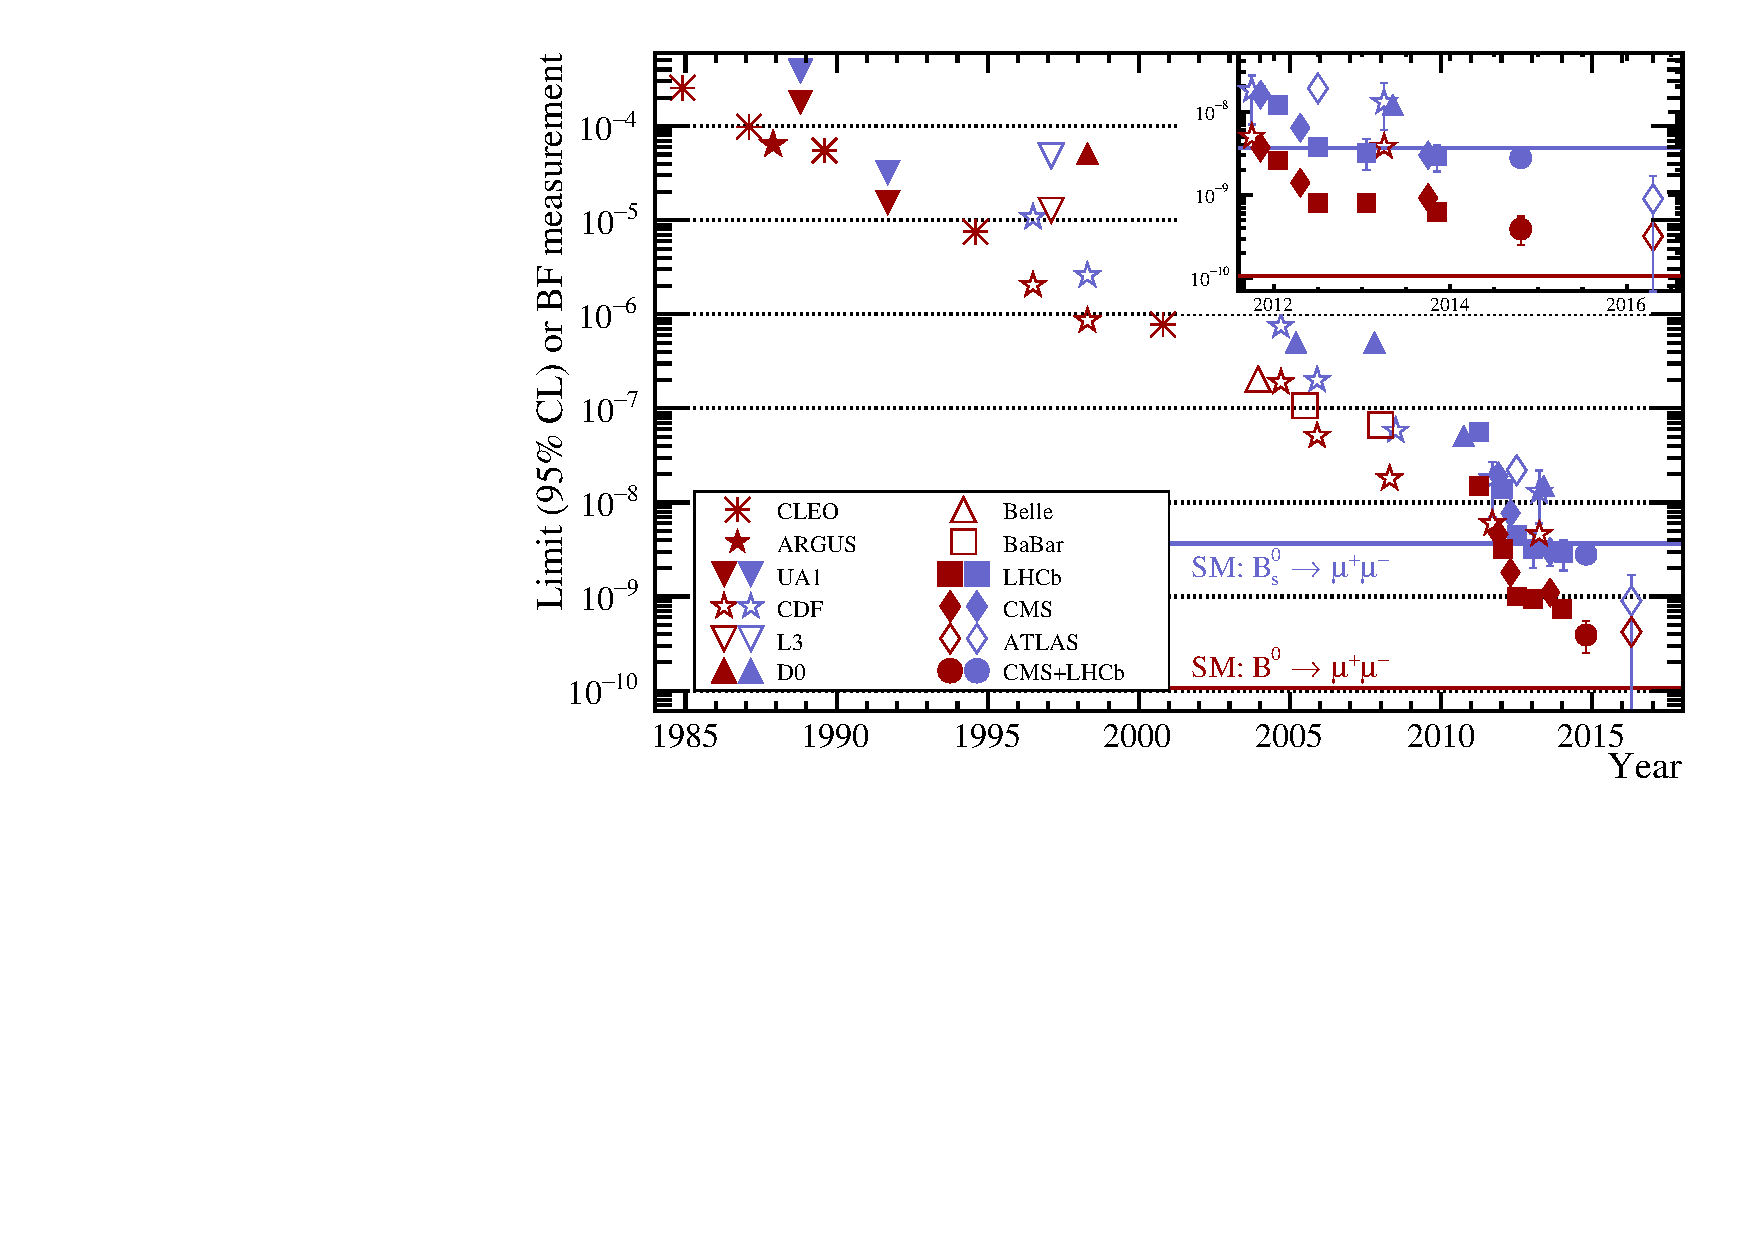
\includegraphics[width=0.8\textwidth]{./Figs/Introduction/95_CL.pdf}
    \caption{Results from searches for \bdmumu (red) and \bsmumu (purple) decays. Upper limits are shown without error bars at the 95$\%$ confindence level. The figure is from reference~\cite{CMS:2014xfa} but updated to include the latest ATLAS result~\cite{Aaboud:2016ire}.}
    \label{fig:bmumu_history}
\end{figure}

The first evidence for \bsmumu decays was found in 2012 by the LHCb experiment~\cite{Aaij:2012nna}. Since then,
the LHCb experiment has measured the \bsmumu \BF to be $\mathcal{B}(B^{0}_{s} \to \mu^+ \mu^-) = (2.9^{+1.1}_{-1.0})\times 10^-9$ at a statistical significance of 4.0$\sigma$ and placed a upper limit on the \bdmumu \BF of $\mathcal{B}(B^{0} \to \mu^+ \mu^-) < 7.4 \times 10^{-10}$ at the 95$\%$ confidence level~\cite{Aaij:2013aka}. The measurements were performed using data collected during 2011 and 2012 at the centre-of-mass energies of 7 and 8 TeV, respectively. Searches for \bmumu decays performed by the CMS experiment using data recorded in the same time period corroborated the results from the results from the LHCb experiment. Producing a measurement of the \bsmumu \BF of $\mathcal{B}(B^{0}_{s} \to \mu^+ \mu^-) = (3.0^{+1.0}_{-0.9})\times 10^-9$ at with a statistical significance of 4.3$\sigma$ and placing a limit on the \bdmumu BF of $\mathcal{B}(B^{0} \to \mu^+ \mu^-) < 1.1 \times 10^{-9}$ at the 95$\%$ confidence level~\cite{Chatrchyan:2013bka}. 
The combined analysis of the CMS and LHCb data sets resulted in the first observation of \bsmumu decays and the first evidence of \bdmumu~\cite{CMS:2014xfa}. The measured branching fractions were measured as
\begin{equation}
\mathcal{B}(B^{0}_{s} \to \mu^+ \mu^-)_{CMS + LHCb}  = 2.8^{+0.7}_{-0.6} \times 10^{-9}
\end{equation}
\begin{equation}
\mathcal{B}(B^{0} \to \mu^+ \mu^-)_{CMS + LHCb}  = 3.9^{+1.6}_{-1.4} \times 10^{-10}
\end{equation}
with a statistical significance of 6.2 $\sigma$ for the \bs mode and 3.0 $\sigma$ for the \bd. The ATLAS experiment also searched for \bmumu decay using data collected during the same period~\cite{Aaboud:2016ire}, measuring the \bsmumu \BF as 
\begin{equation}
\mathcal{B}(B^{0}_{s} \to \mu^+ \mu^-)_{ALTAS}  = 0.9^{+1.1}_{-0.8} \times 10^{-9}
\end{equation}
with a statistical significance of 2~$\sigma$. An upper limit was placed on the \bdmumu decay of $\mathcal{B}(B^{0}_{s} \to \mu^+ \mu^-) >4.2 \times 10^{-10}$ at the 95 $\%$ confidence level.
Although it was hoped that large deviations from the SM predictions would be found in these decays this has not been observed. 
All the measured values are consistent with the expectations of the SM and have enabled constraints to be placed on the parameter space available for new physics models. Nevertheless, the precision of the measurements allows plenty of room for NP effects to be revealed. Furthermore there is some tension between both the separate measurements and each measurement and the SM prediction as shown in Figure~\ref{fig:contour}. 
\begin{figure}[htbp]
    \centering
        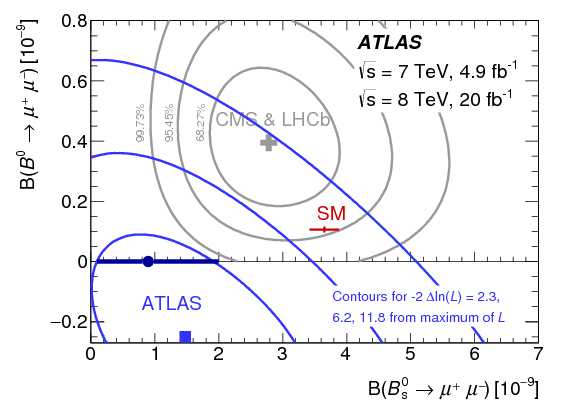
\includegraphics[width=0.8\textwidth]{./Figs/Introduction/contour_plot.png}
        \caption{Measurements of the \bdmumu \BF and \bsmumu \BF from the ATLAS experiment and the combined analysis of CMS and LHCb data alongside the predictions of the SM~\cite{Aaboud:2016ire}. The measurements were performed using data collected during 2011 and 2012 and centre-of-mass energies of 7 and 8~\tev, respectively.}
        \label{fig:contour}
\end{figure}
%The measurements have enabled strong constraints to be placed on the parameter space available for new physics models~\cite{} but the precision of the measurements still allows plenty of room for NP effects to be revealed. 
Therefore the study of \bmumu decays continues to be an very interesting topic in the search for NP effects. 

The data collected during Run 2 of the LHC, where the centre-of-mass energy of $pp$ collisions is increased to 13 TeV, will enable more precise measurements of the \BFs of these decays to be made. 
Furthermore the observation of \bsmumu decays opens the way for other properties of this decay to be studied. In particular the effective lifetime of \bsmumu decays provides a complementary search for NP effects to the \BF measurement, the presence of new physics effects could be revealed in either both or only one of these measurements. The search for \bsmumu decays is over and the study of this decay has begun.



This dissertation documents the latest study of \bmumu decays at the LHCb experiment. The measurements of the \bmumu \BF and the \bsmumu effective lifetime are presented using data collected during $pp$ collisions with centre-of-mass energies of 7, 8 and 13~\tev. The theoretical motivation for studying these decays is given in Chapter~\ref{sec:theory_chptr} and the LHC and LHCb experiment are described in Chapter~\ref{CERN_LHC_LHCb}. The criteria used to identify these decays in the data collected by the LHCb experiment are detailed in Chapter~\ref{selection_chapter} and the measurement of the \BF is briefly covered in Chapter~\ref{sec:BFanalysis}. The measurement of the effective lifetime is discussed in Chapter~\ref{sec:lifetimemeasurement} and the systematic uncertainties on this measurement are given in Chapter~\ref{sec:systematics}. Finally a summary of the results and prospects for future measurements of \bmumu decays are given in Chapter~\ref{sec:summaryandoutlook}.


\mainmatter
\chapter{CERN, the LHC and LHCb}
\label{CERN_LHC_LHCb}

The European Organisation for Nuclear Research (CERN) was founded in 1954 and began with 12 member states as a organisation to encourage European collaboration and the study of nuclear physics. Since it's foundation the collaborative nature of CERN allowed for large-scale expensive experiments and machines to be built. The Proton Synchrotron was CERN's flagship accelerator, operational in 1959 it had a circumference of 628~m and accelerated protons to 25 \gev, the highest energy at that time. Now 62 years since it's foundation CERN has grown to include 21 member states \footnote{about the other types of countries involved.} and is still at the forefront of high energy physics research. CERN’s latest accelerator, the Large Hadron Collider (LHC), is most energetic particle accelerator ever built, with a 27~km circumference the LHC was designed to protons at 14 \tev. This chapter shall discuss the LHC and the LHC beauty experiment, one of the experiments that uses collisions provided by the LHC.

\section{The LHC}
\label{LHC}


The LHC is a proton synchrotron that was designed to accelerate and collide two beams of protons travelling in oposite directions up to a center-of-mass energy of 14 \tev. Although operation of the LHC began in 2010 it is yet to reach design energy. The purpose of the LHC is to provide high energy proton collisions, the products of which are used for precision tests of the Standard Model (SM) and to search for new physics particles that go beyond the scope of the SM. There are four interaction points on the LHC ring where the beams are brought to collide, at these points various experiments detect and study the products of these collisions. The LHC can also accelerate lead-nuclei up to an energy of 2.76 \tev per nucleon, but it is only the products from proton collisions that are the topic of this thesis.

%It's the bit below that I'm not a massive fan of the explains how the LHC gets it's protons. I think that it is a little too brief and disconnected with not explainations.
The protons for the LHC originate from hydrogen gas, %add something nice here
the hydrogen atoms are ionised to strip away the electrons and the protons are accelerated through a chain of particle accelerators of increasing energy before being injected into the LHC. The chain of accelerators, shown in Fig.~\ref{fig:accelerator_chain}, consists of existing accelerators that have been used in various experiments through the second half of the last century and have been upgraded to meet the requirements needed to providing protons for the LHC. 
The protons leave the chain of accelerators with of energy of 450 \gev per proton and in bunches of >~$10^{11}$, as the bunches injected into the LHC they are split into two oppositely circulating beams.
The LHC accelerates the protons to the desired center of mass energy using supercooled radio frequency cavities for acceleration and superconducting dipole magnets to bend the beams around the ring. %I could add here some details about the magnets and how the LHC accelerates the protons.
Once the required energy has been reached, the bunches are focused using quadrupole magnets before being brought to collide at 4 interaction point at a bunch crossing rate of 40 MHz. 


\begin{figure}[htbp!] 
  \centering    
  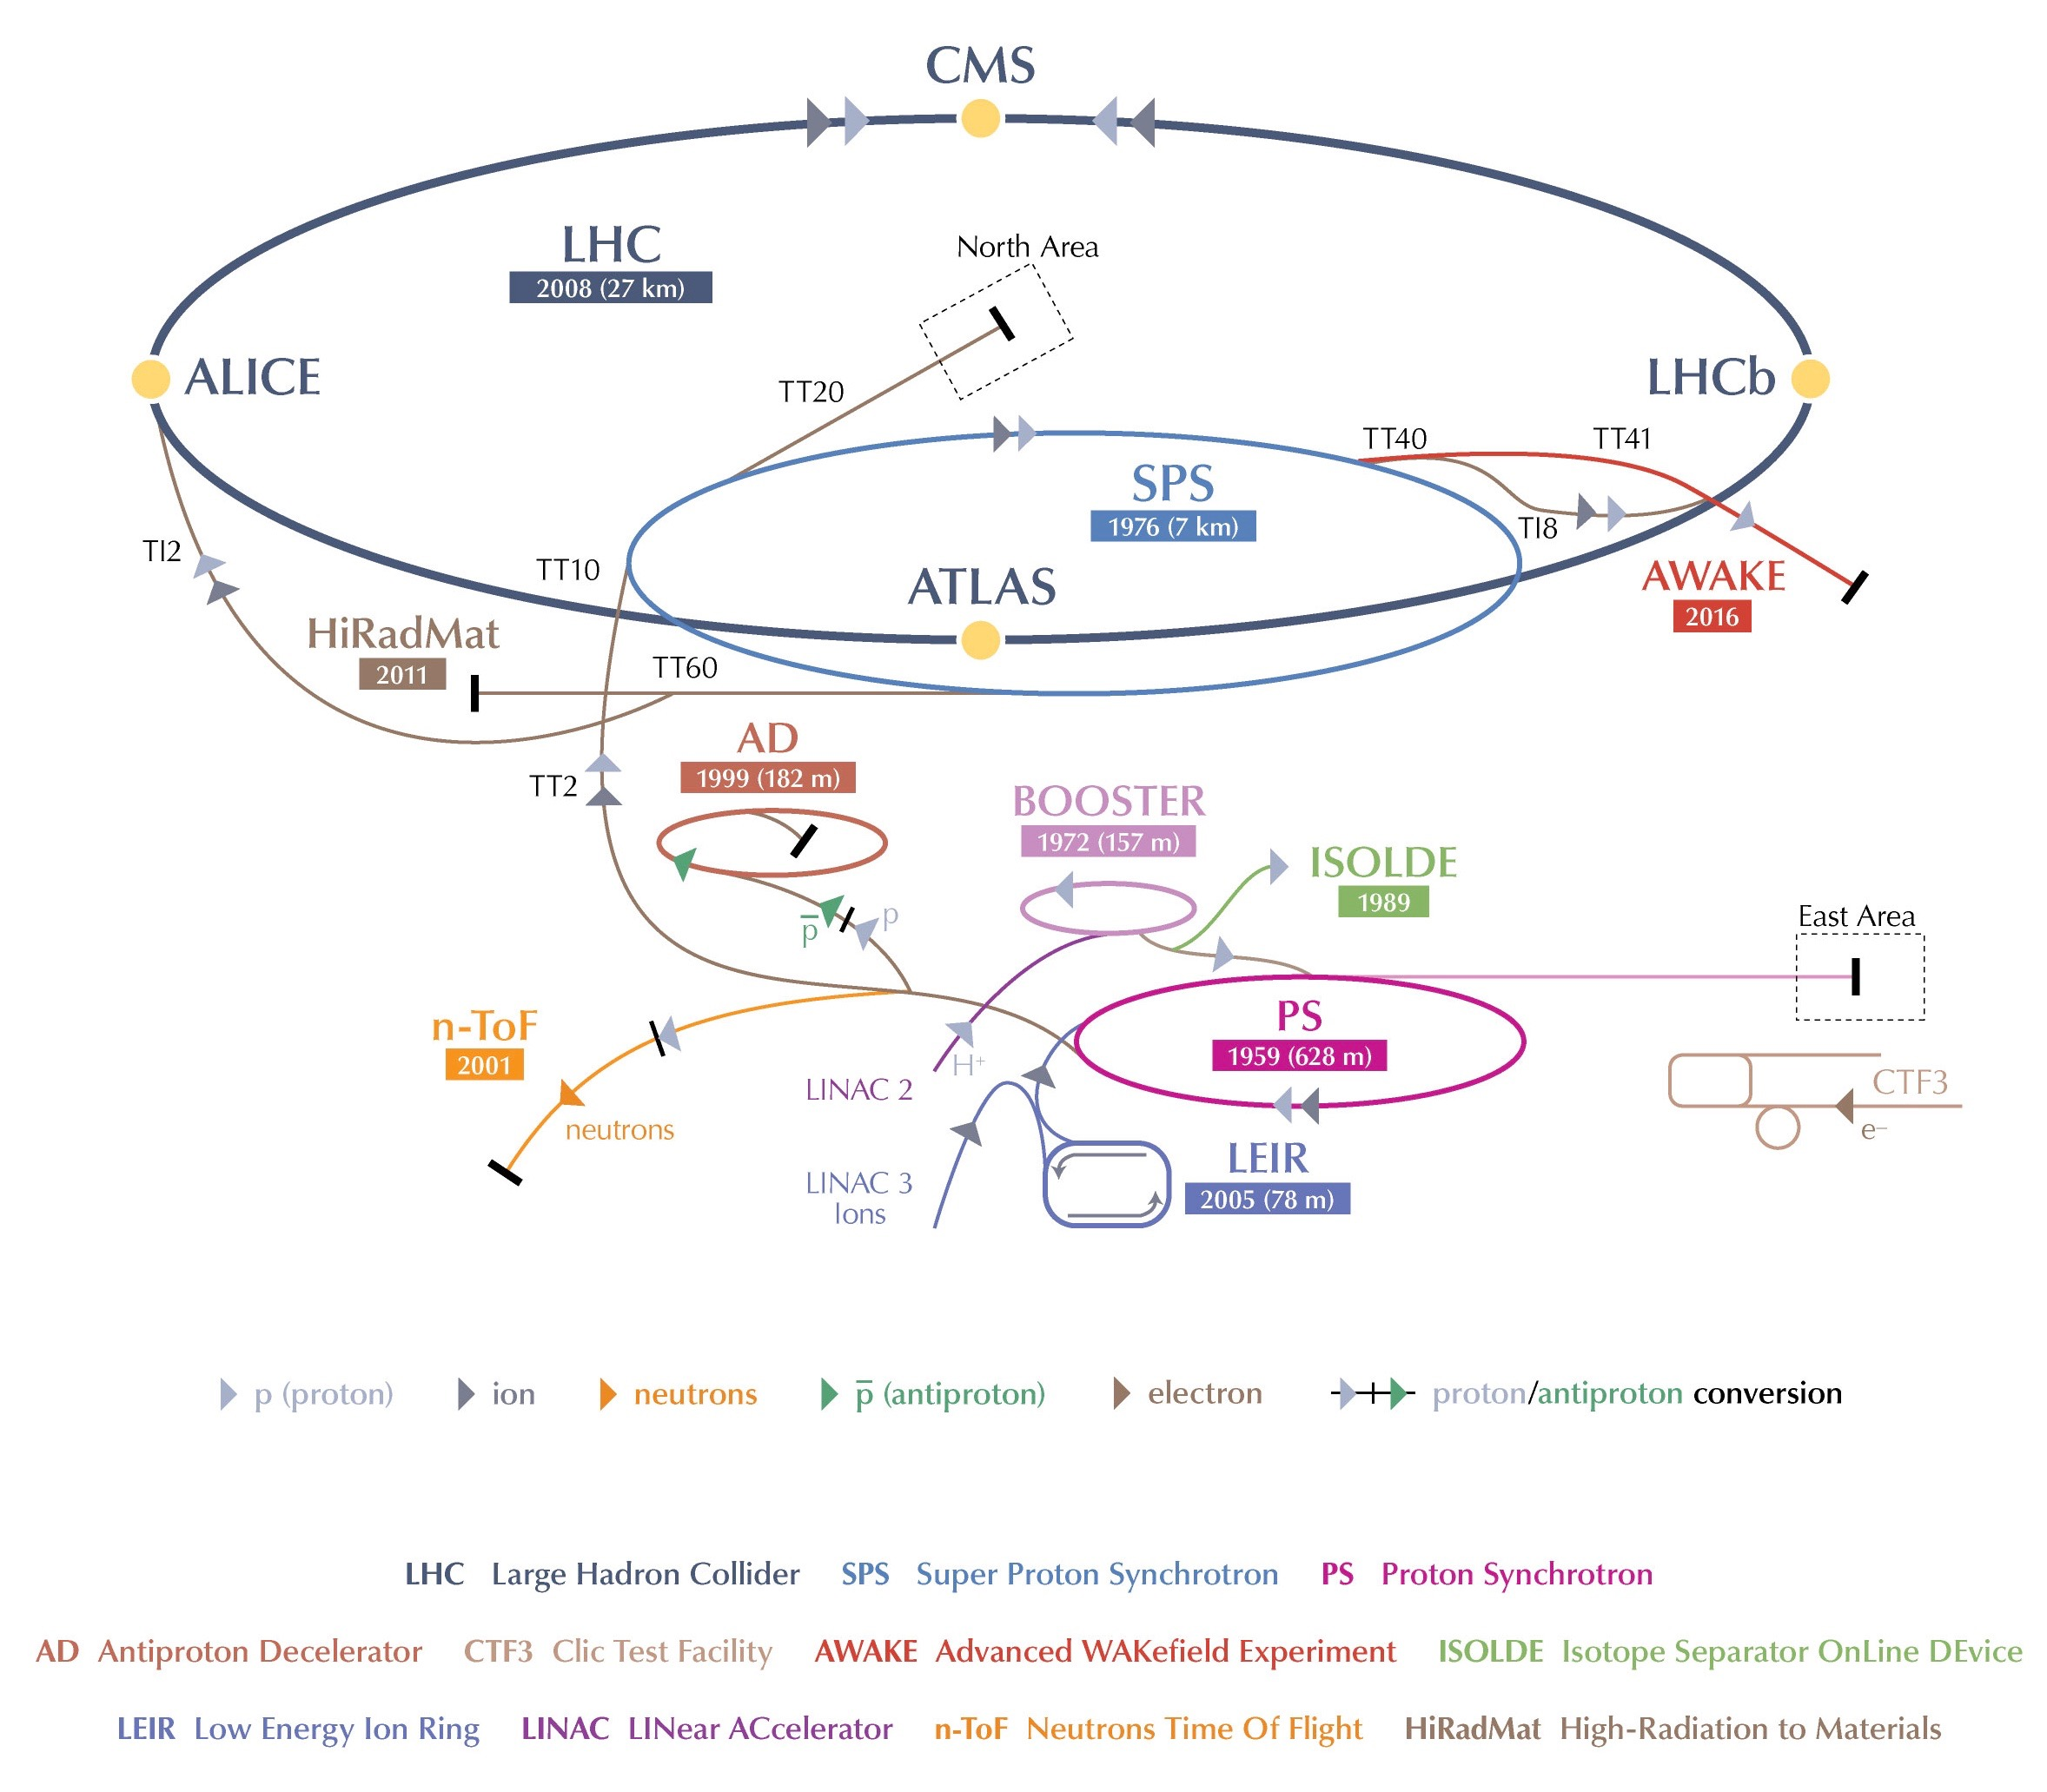
\includegraphics[trim = 125mm 2mm 125mm 90mm, clip, width=1.0\textwidth]{accelerator_complex.jpg}
  \caption{The accelerator complex at CERN. The chain of accelerators used to inject protons into the LHC consists of the Linac 2 accelerating protons to 50 \mev, the Proton Synchrotron Booster accelerating protons to 1.4 \gev, the Proton Synchrotron accelerating protons to 25 \gev and creating the desired spacing between proton bunches then finally the Super Proton Synchrotron accelerating protons to 450 \gev. Source: CERN.}
  \label{fig:accelerator_chain}
\end{figure}




The CoM energy of a collider is an important measure of it's preformance as it dictates what particles can or could be produced in collisions but another important measure of collider performance is the instantaneous luminoscity a collider can provide. The instantaneous luminoscity, $\mathcal{L}$, is a meaure of how many collisision occur per second, it is given by

\begin{equation}
\mathcal{L} = \frac{N^{2} f n_{b}}{\mathcal{F}}.
\label{eq:inst_lumi}
\end{equation}

where $N$ is the number of protons per bunch, $n_{b}$ the number of bunches per beam, $f$ the bunch revolution frequency and $\mathcal{F}$ contains information about the beam geometry. The LHC is designed to operate at a maxiumum instantaneous luminoscity of $10^{34}$ cm$^{-2}$s$^{-1}$, in order to reach this luminoscity the LHC can have 2808 bunches per beam and a revolution frequency for beams is 11.245 kHz leading to a seperation of 25 ns between bunches. The higher the luminoscity, the more collisions happen in a second and the more particles will be produced, this can either be advantageous or disadvantageous depending on the physics process that is being studied.
% and the detector design that records the collisions. 
Therefore luminoscity delivered at each interaction point can be tuned by the quadrupole magnets by altering the shape of each bunch to suit the experiments at each point.



%Detector on the LHC
There are 7 experiments on the LHC that detect the particles produced in proton and heavy ion collisions. There are two general purpose detectors, ATLAS and CMS, that were designed to search for the Higgs boson and new particles that are beyond the scope of the SM in proton collisions, these two experiments operate at the full instantaneous luminoscity of the LHC. %Prehaps say we found the Higgs?
ALICE studies quark-gluon plasma produced in heavy ions collisions in order to probe conditions similar to the early universe. TOTEM studies properties of protons as they collide head on at the LHC. MOEDAL is designed primerally to detect magnetic monopoles, particles carrying magnetic charge which are so far unobserved. LHCf is a very foward experiment that is designed to detect particles that are thrown forward in LHC collisions which would simulate processes similar to those occuring in cosmic rays. Finally there is the Large Hadron Collider Beauty experiment (LHCb), this experiment was designed to studies rare $b$-hadron decays and $\mathcal{CP}$ violating processes and operates at a lower luminoscity that the general purpose detectors. The data collected by LHCb is the focus of this thesis.


%Operation of the LHC and what has been delivered to LHCb






\section{The LHCb Experiment}
%\cite{LHCb}
The LHCb detector is designed specifically to study $CP$ violation and rare decays of $b$-hadrons and $c$-hadrons building on work done a the B factories and the Tevatron.
At the high energies the LHC operates at $b\bar{b}$ pairs are produced together at low polar angles in either the forwards or backwards cone along the 
beam direction. The detector is designed as a single-arm spectrometer to take advantage of this behaviour.


A cross-section of the detector layout is shown in Fig.~\ref{LHCb}. 

\begin{figure}[htb]
\centering
  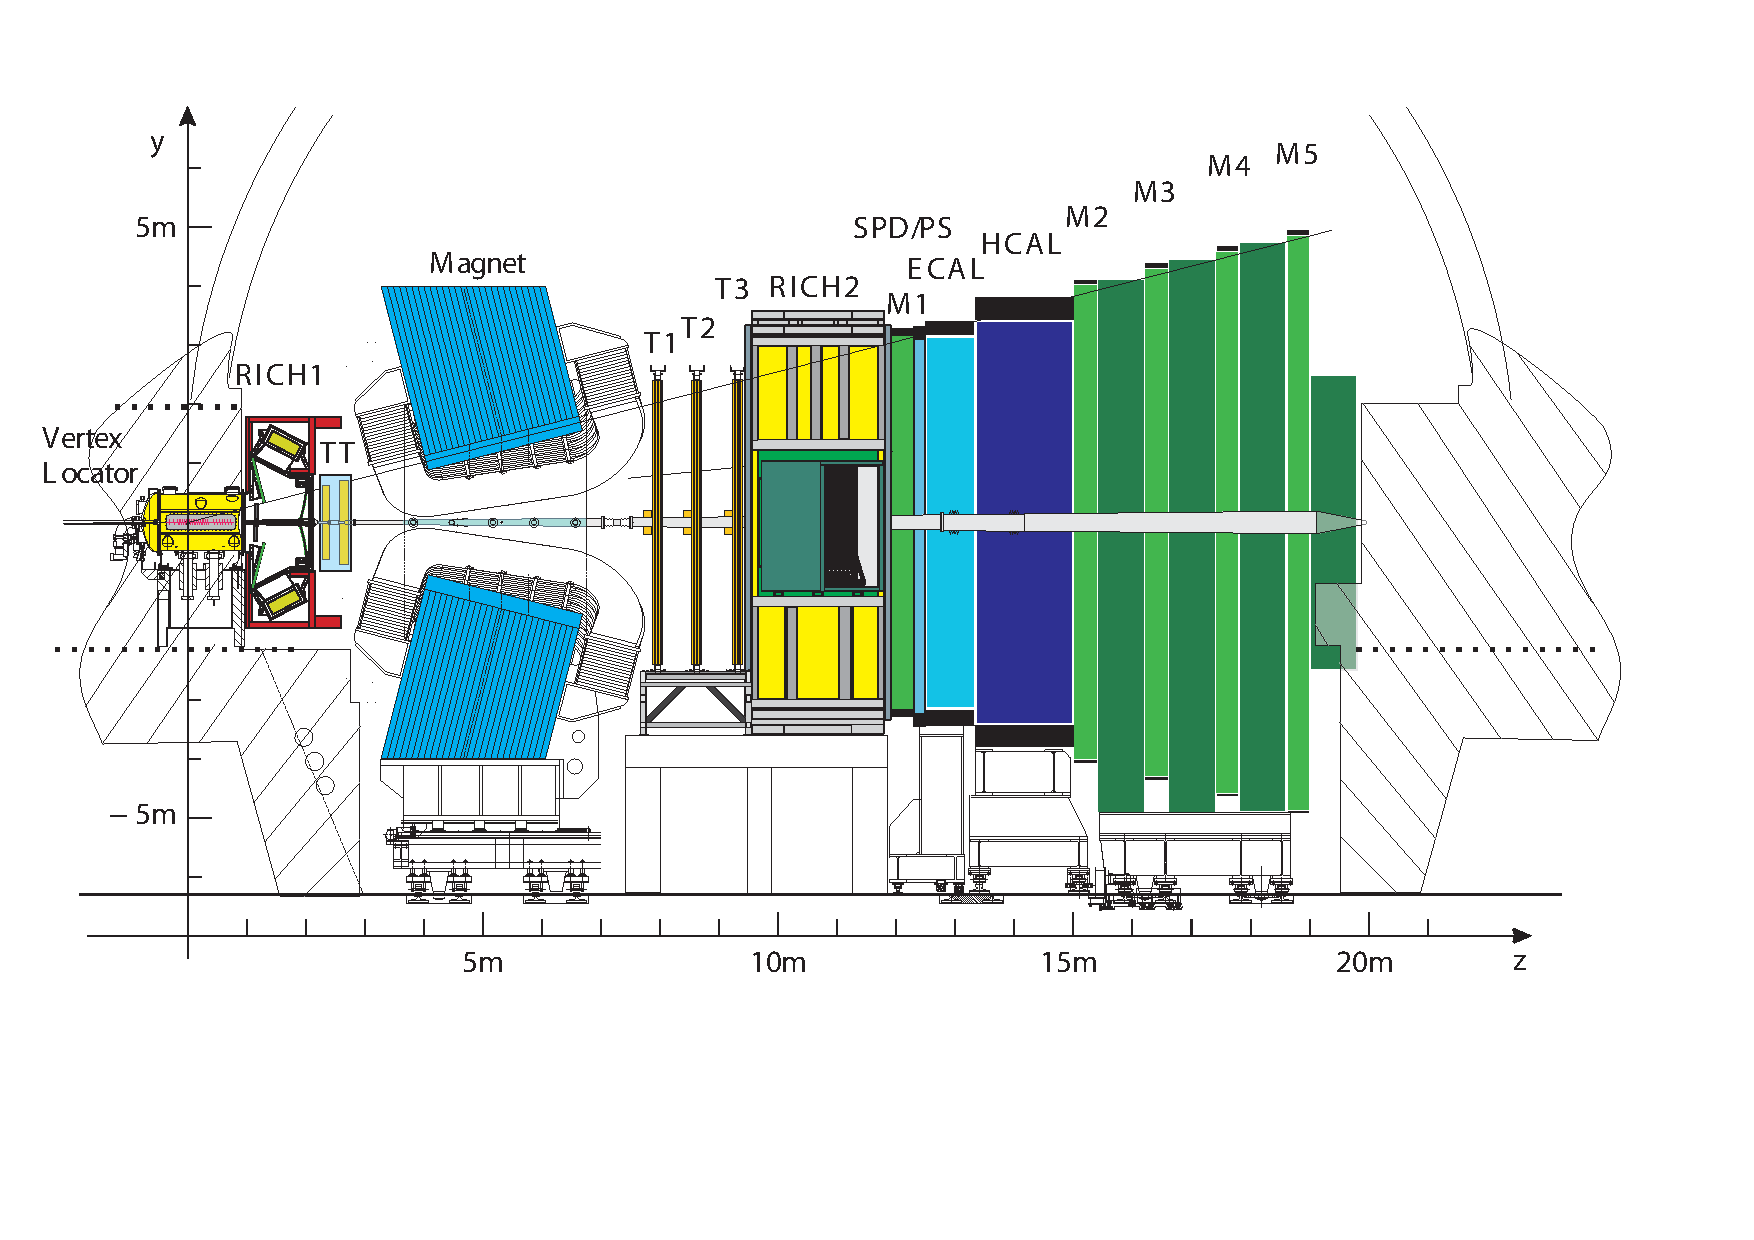
\includegraphics[width = 0.85 \linewidth]{lhcb.pdf}
  \caption{Cross-section of the LHCb detector the the $z$-axis is along the beam pipe and the $y$-axis is the vertical direction \cite{LHCb}.}
  \label{LHCb}
\end{figure}

The LHCb detector is composed of sub-detectors with different design purposes. The vertex locator (VELO) 
and the tracking stations (TT, T1, T2 and T3) are key for tracking charged particles travelling through
the detector. The RICH detectors, calorimeters (ECAL, HCAL, PS and SPD) and the muon stations (M1-5) 
are necessary for particle identification. The dipole magnet in the detector is used alongside the tracking stations in order to measure particle charge and momentum.


The VELO is the tracking detector closest to the interaction point. It is designed to locate primary and secondary decay vertices. Secondary vertices occur within the VELO
due to the short lifetime of $b$-hadrons, whereas primary vertices do not occur in the VELO but tracks in the VELO are extrapolated backwards to determine the vertex location.
The VELO is a silicon micro-strip detector which give good resolution of tracks and decay vertices. 




The T1-3 tracking station consist of the Inner Tracker (IT) and the Outer Tracker (OT). The IT is a silicon micro-strip detector and makes up the inner sections of the stations closest to the beam pipe.
The OT is a straw-tube drift-chamber and covers the outer sections of the T1-3 stations. Silicon micro-strip detectors are needed in the IT due to high particle occupancy however the particle flux is lower at large polar angles from the beam pipe allowing straw tubes to be used
in the OT as the occupancy is lower. The Tracker Turicensis (TT) is also a silicon micro-strip detector upstream of IT and OT, it spans the full acceptance of the LHCb detector. The TT, IT and OT work together with the dipole magnet to measure charge and momentum of particles travelling through the detector. Obtaining good momentum resolution is vital because the momentum resolution 
directly affect the invariant mass resolution of reconstructed particles. 

Distinguishing between $e$, $\mu$, p, K, $\pi$ and photons is important for accurately reconstructing particle decays. Each sub-detector related to particle identification is specialised for
 different particles. The sub-detectors for particle identification are the two RICH detectors, the Preshower detector (PS), Scintillating Pad Detector (SPD), the electromagnetic calorimeter (ECAL), the hadronic calorimeter 
(HCAL) and the muon tracking stations (M1-5). 

The particle identification detectors closest to the interaction point are the RICH~1 and RICH~2. These detectors are ring imaging $\check{\text{C}}$erenkov detectors, designed to separate charged pions and kaons
 which are produced in large number from $b$-hadron decays.  In LHCb, high momentum particles are produced at small polar angles and lower momentum particles at larger polar angles, therefore two RICH 
detectors are needed to cover the full momentum and acceptance range. The RICH 1 is composed of an areogel and $C_{4}F_{10}$ gas radiator, it is sensitive to particles with momentum between  1 and 60 G$e$V/$c$. 
The RICH 2 is a $CF_{4}$ gas radiator and is sensitive to particles with momentum between 15 and 100 G$e$V/$c$. 


The SPD distinguishes charged and neutral particles such as photons and electrons which leave the same signals in the ECAL. The PS detector distinguishes electrons and 
charged pions by utilising their different interaction lengths in matter. 


Downstream of the SPD and the PS is the ECAL, a lead-scintillator sampling detector. Electrons and photons interact within the lead producing electromagnetic showers, the scintillator 
absorbs photons produced by the showers and emits photons at different wavelengths so that photomultiplier tubes detect them. The energy of an incident particle is measured from the energy of the shower which is proportional to the light produced in the shower. Showers produced by photons can be distinguished from those produced by electrons because photons leave no hits 
in the tracking detectors or the SPD. Hadrons will pass though the ECAL to be detected by the HCAL. The HCAL is composed of lead and scintillator tiles and measure the energy 
hadronic showers produced inside it. The HCAL works in the same way as the ECAL however the lead absorber is more suited to producing hadronic showers rather than electromagnetic ones.

Muon identification is key for the analysis of several important CP violating decays and rare decays, including $B_{s} \to \mu^{+} \mu^{-}$. The ECAL and the HCAL absorb most particles produced in collisions. 
However, the high penetration power of muons allows then to pass through the ECAL and HCAL therefore the muon stations can be the in furthest part of the detector.  The muon stations are multi-wire proportional chambers except the inner part of the M1 station which is 
a gas electron multiplier due to the high particle occupancy. 


Muon identification is not only important for offline analysis but, together with information from the ECAL and HCAL, the muon system triggers events which are saved for offline analysis. 
The LHCb has been designed to operate at a lower instantaneous luminosity than the running of the LHC, the trigger takes the 10 MHz of data visible in the LHCb and reduces it to 5 kHz which can 
be stored offline. There are two levels to the trigger the Level 0 (L0) and the High Level Trigger (HLT). The L0 operates at the same time as the bunch crossings and reduced the rate to 1 MHz
by using transverse momentum information from the ECAL, HCAL and the muon stations. The HLT further reduces the rate to 5 kHz, running asynchronously with the bunch crossings on a processor farm. The HLT
takes events that have been triggered by the L0 and confirms them by reconstructing the events more fully using information from the VELO and other tracking stations. Once the data has been stored there are further offline selections
which aim to further reduce the background and enhance the signal for particular decays.  The trigger is optimised so when it is combined with the offline selection it can give the best signal and best background rejection. Since the LHCb studies many different decays there are various different
triggers that are used for different analyses. 




%Things to note and change:
%The IT and OT it's not really about resolution but about occupancy. There can only be one event hit per strip so that the reading makes sense and isn't useless. If a straw tube, which is 
%v long, gets more that 1 hit the readout is useless, since there are more particles in at small polar angles we need more/smaller detectors so that the occupancy of each detector is smaller.
%Can't have SMD over all the detector because it is too expensive.

%The trigger number are probably wrong now, it was bten 4 and 6 kHz in 2012. Also would be good to add in more details about how the trigger works. 

%Add in that the PS-HCAL get rid of all/many the other particles which are not muons therefore allowing the M2-5 to detect what is left which are muons.


\chapter[Theory of $B\to \mu^+ \mu^-$ decays; the Standard Model and beyond]{Theory of \boldmath{$B\to \mu^+ \mu^-$} decays; the Standard Model and beyond}
\label{sec:theory_chptr}
This Chapter describes the theoretical motivation for the study of \bmumu decays. 
The description of these decays within the SM framework is presented in Section~\ref{sec:bsmumu_in_SM} and the determination of the theoretical predictions of \BFs is outlined in Section~\ref{sec:BFdef}.
The discussion of the theoretical \BFs is based on references~\cite{Blake:2016olu,Anikeev:2001rk}. 
Quark mixing leads to oscillations of a \bs to a \barbs over time and a difference between the values of the predicted and measured \bsmumu \BFs. These oscillations and the influence on the \BFs values are described in Section~\ref{sec:quarkmaixing} and follows the material in refereneces~\cite{Dunietz:2000cr, Anikeev:2001rk,Nierste:2009wg}. 
A new parameter, \ADG, arises from the \bs - \barbs oscillations and it can be measured through the effective lifetime of \bsmumu decays as described in Section~\ref{sec:ADG_EL}. The SM predictions for \BFs and the effective lifetime are given in Section~\ref{sec:SM_predictions} and the ways in which NP can influence these observables is briefly discussed in Section~\ref{sec:NPmodels}.



\section[$B^0_{(s)}\to \mu^+ \mu^-$ decays in the Standard Model]{\boldmath{$B^0_{(s)}\to \mu^+ \mu^-$} decays in the Standard Model}
\label{sec:bsmumu_in_SM}
%Prehaps I should mention anti-particles earlier?
In the SM, quarks and anti-quarks can be combined in pairs to form mesons that are held together by the strong force. The neutral $B$ mesons, \bd and \bs, are made up of a $\bar{b}$ quark combined with a $d$ quark for the \bd and an $s$ quark for the \bs. Their anti-particles, \barbd and \barbs, are formed by swapping over which quark flavour in the pair is the anti-quark. These particles are unstable and exist for $\sim10^{-12}$~s before decaying into leptons, lighter mesons or a combination of both. One decay mode is when the \bsd decays into two oppositely charged muons as \bmumu~\footnote{\bmumu refers to both the particle and anti-particle decays of the \bd and \bs unless otherwise specified.}. This decay mode occurs very rarely in the SM compared to other decay modes of the \bsd, the suppression of this mode arises from several different sources.

The composite quarks of a \bsd both have the same charge, therefore in the decay \bmumu only quark flavour and not quark charge changes. This type of decay is called a flavour changing neutral current (FCNC). These decays must proceed via the weak force because it is the only interaction in which quark flavour is not conserved via the exchange of a $W$ boson. However, FCNCs are forbidden in the SM to occur at the tree level by the GIM mechanism~\cite{PhysRevD.2.1285}. Therefore \bmumu decays proceed via $W$-box and $Z^0$-penguin diagrams as shown in Figure~\ref{fig:SM_diag}.

\begin{figure}[htbp]
    \centering
        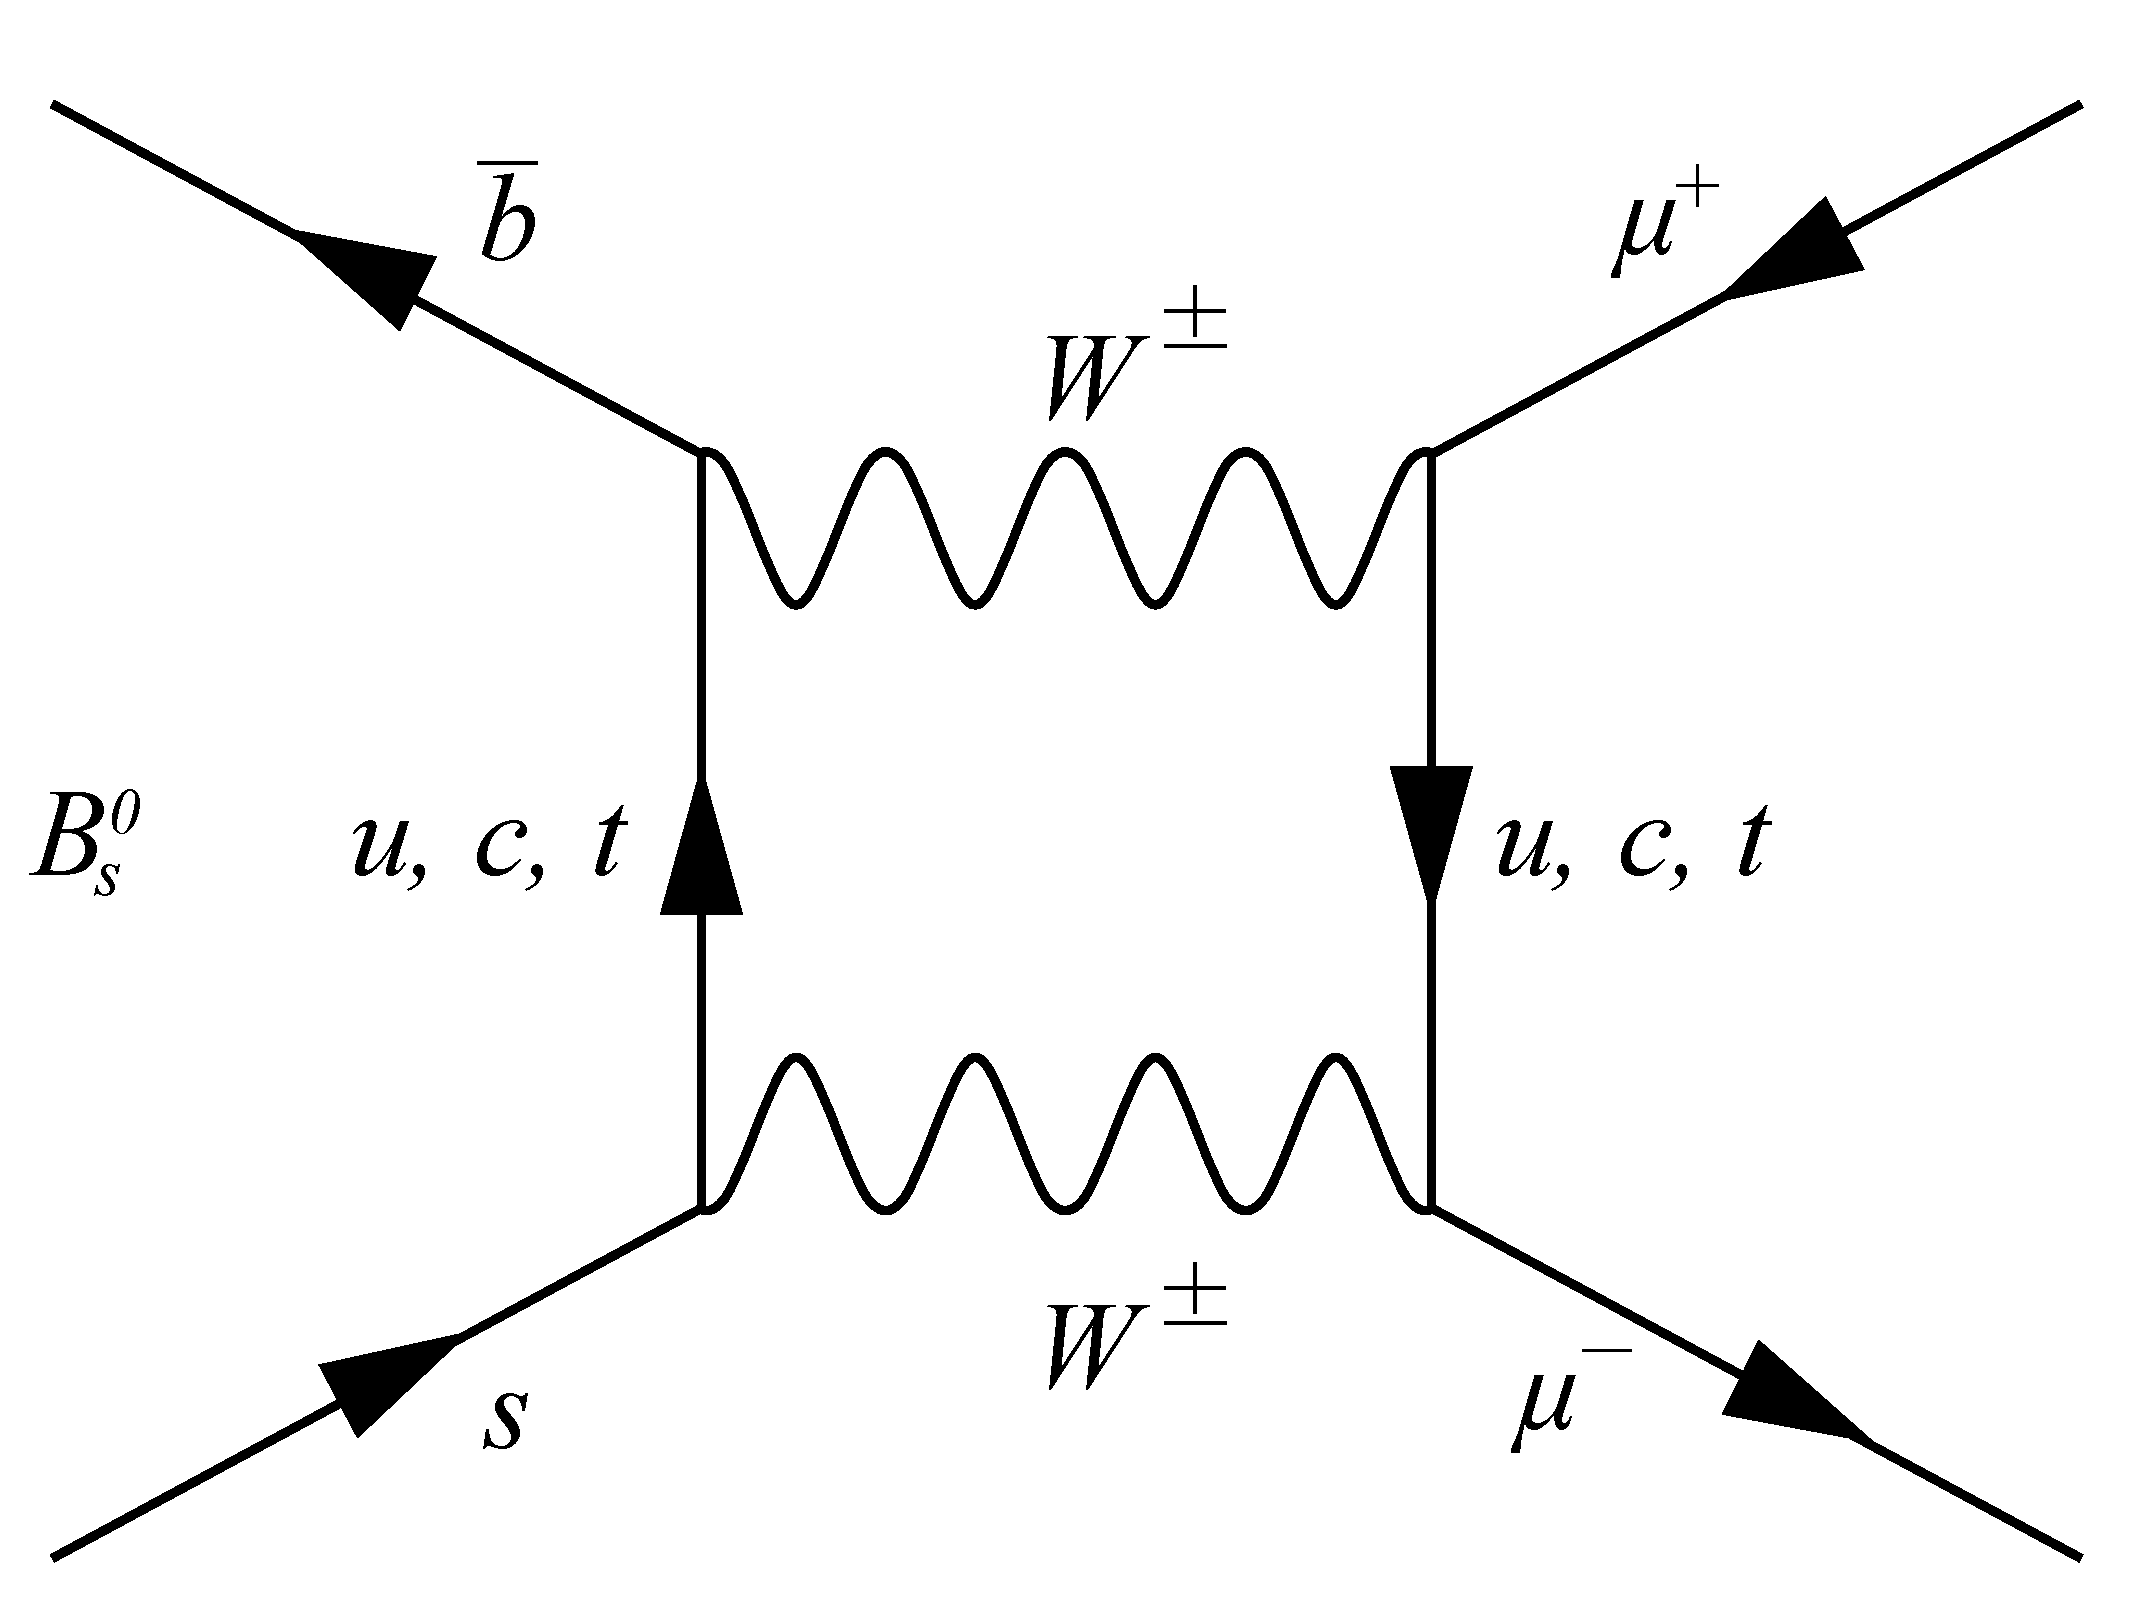
\includegraphics[width=0.4\textwidth]{./Figs/Theory/W_diagram.pdf}
        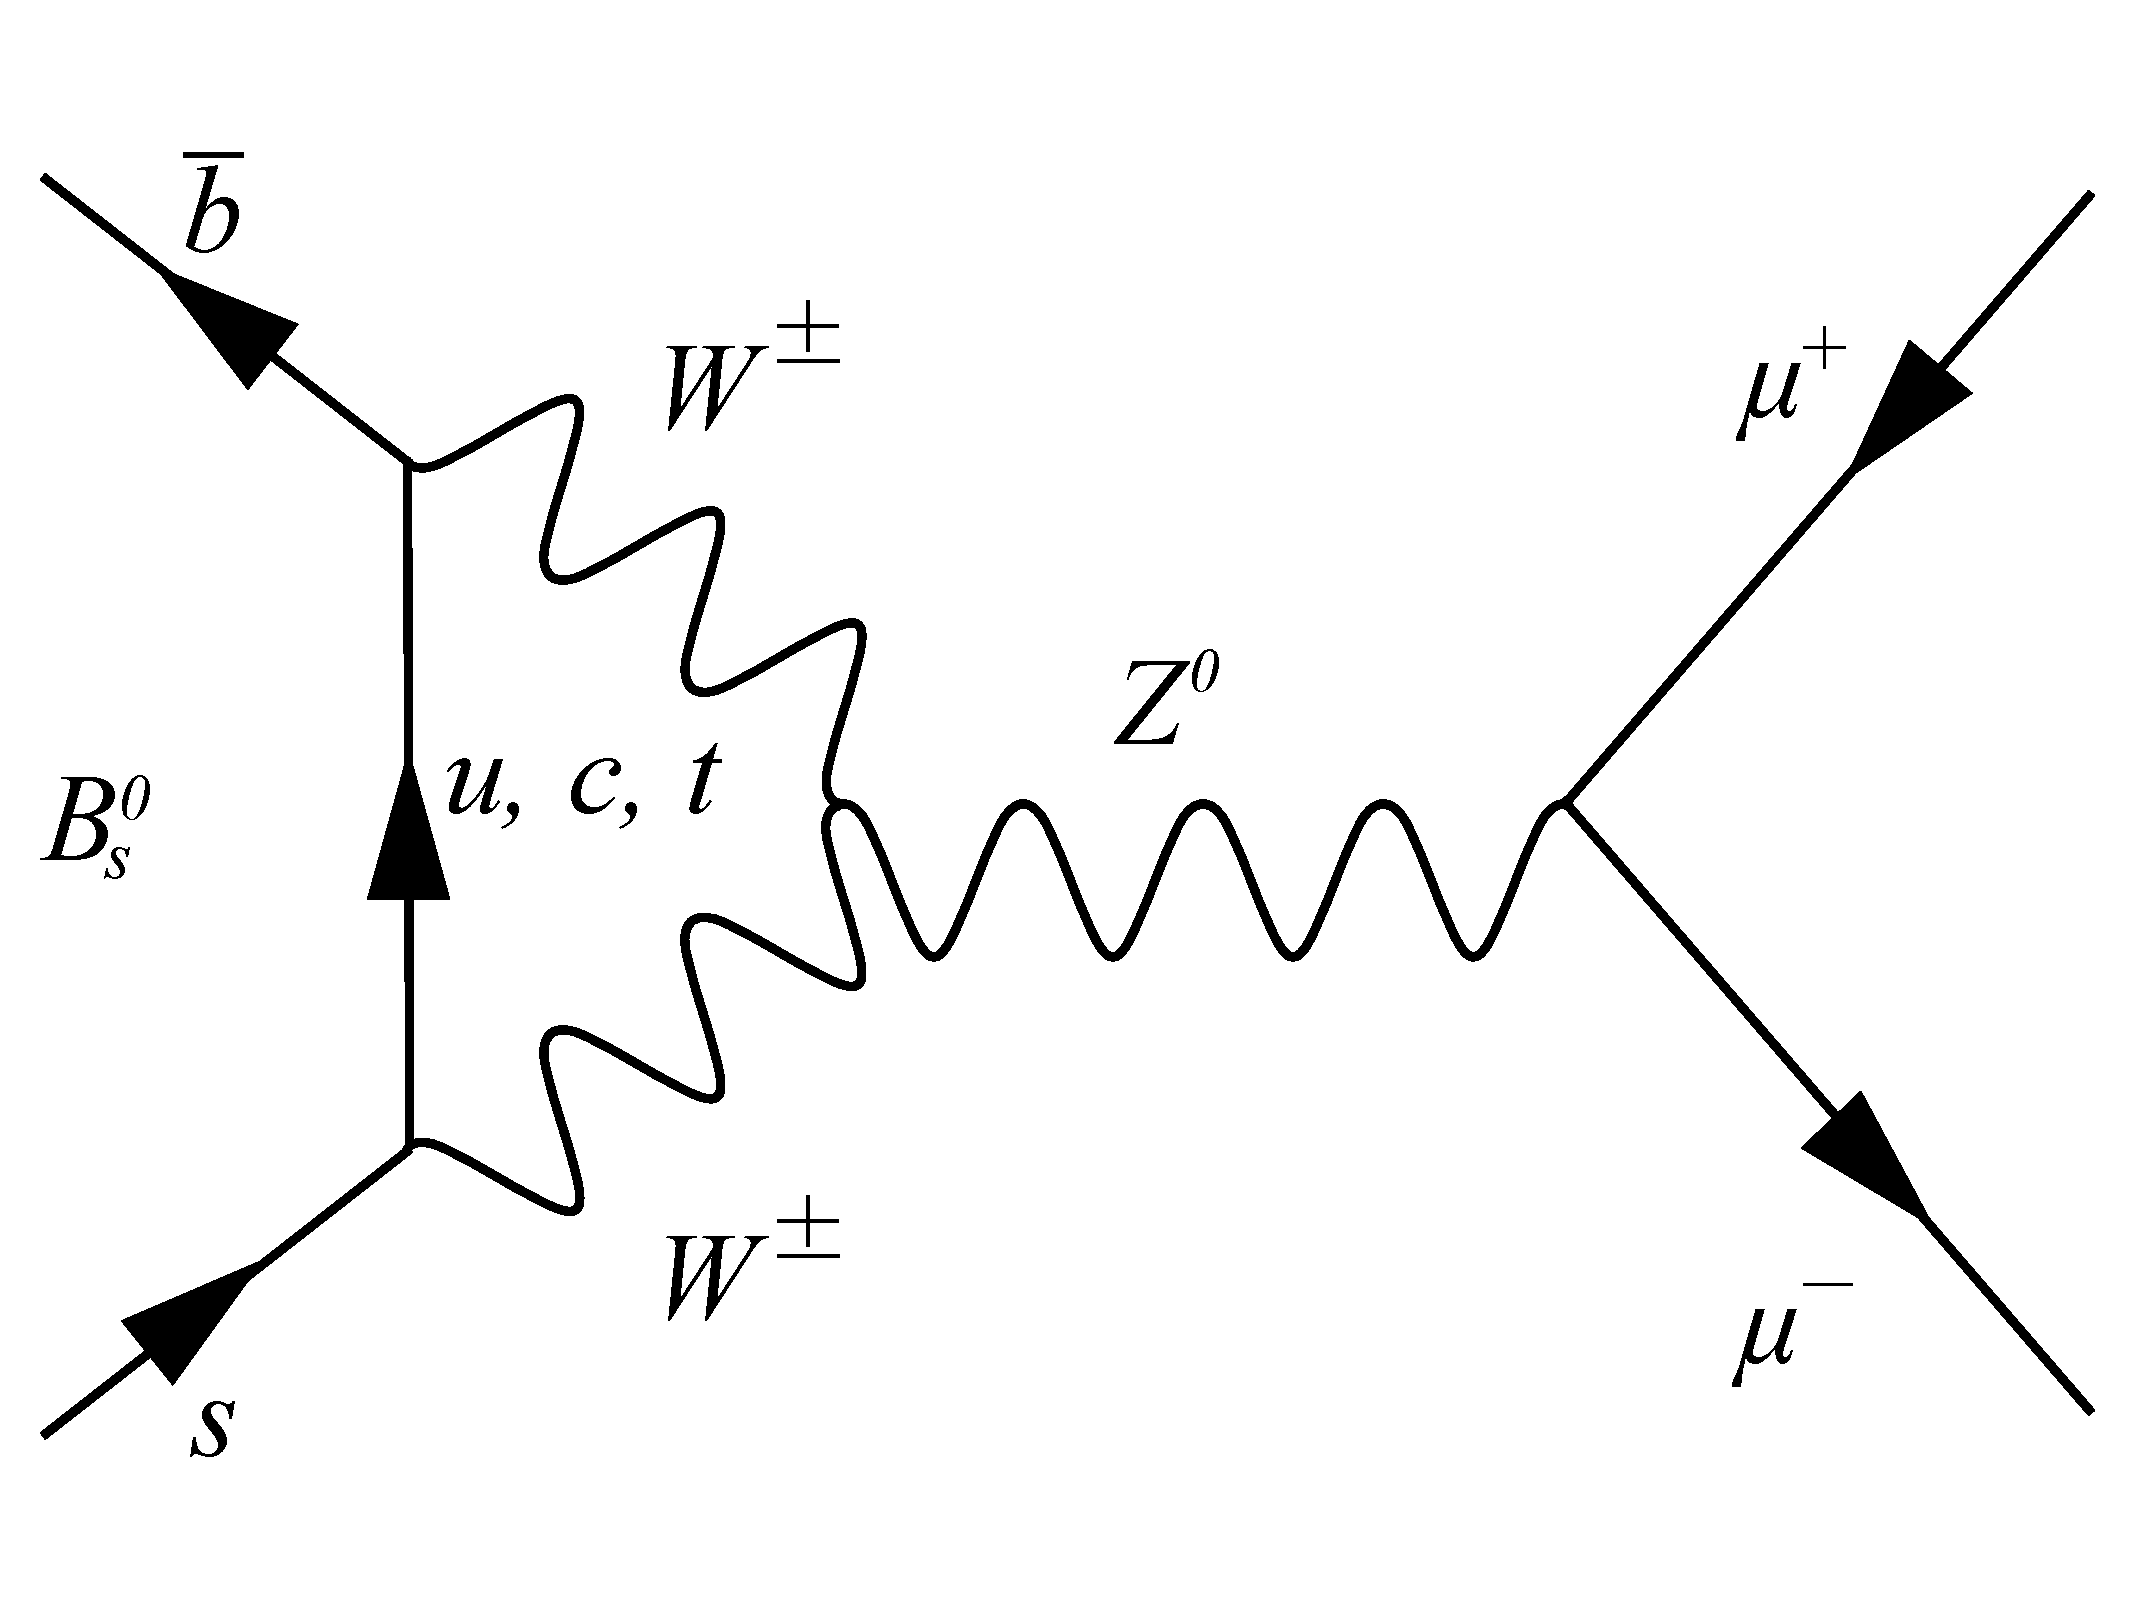
\includegraphics[width=0.4\textwidth]{./Figs/Theory/Z0_penguin_v1.pdf}
        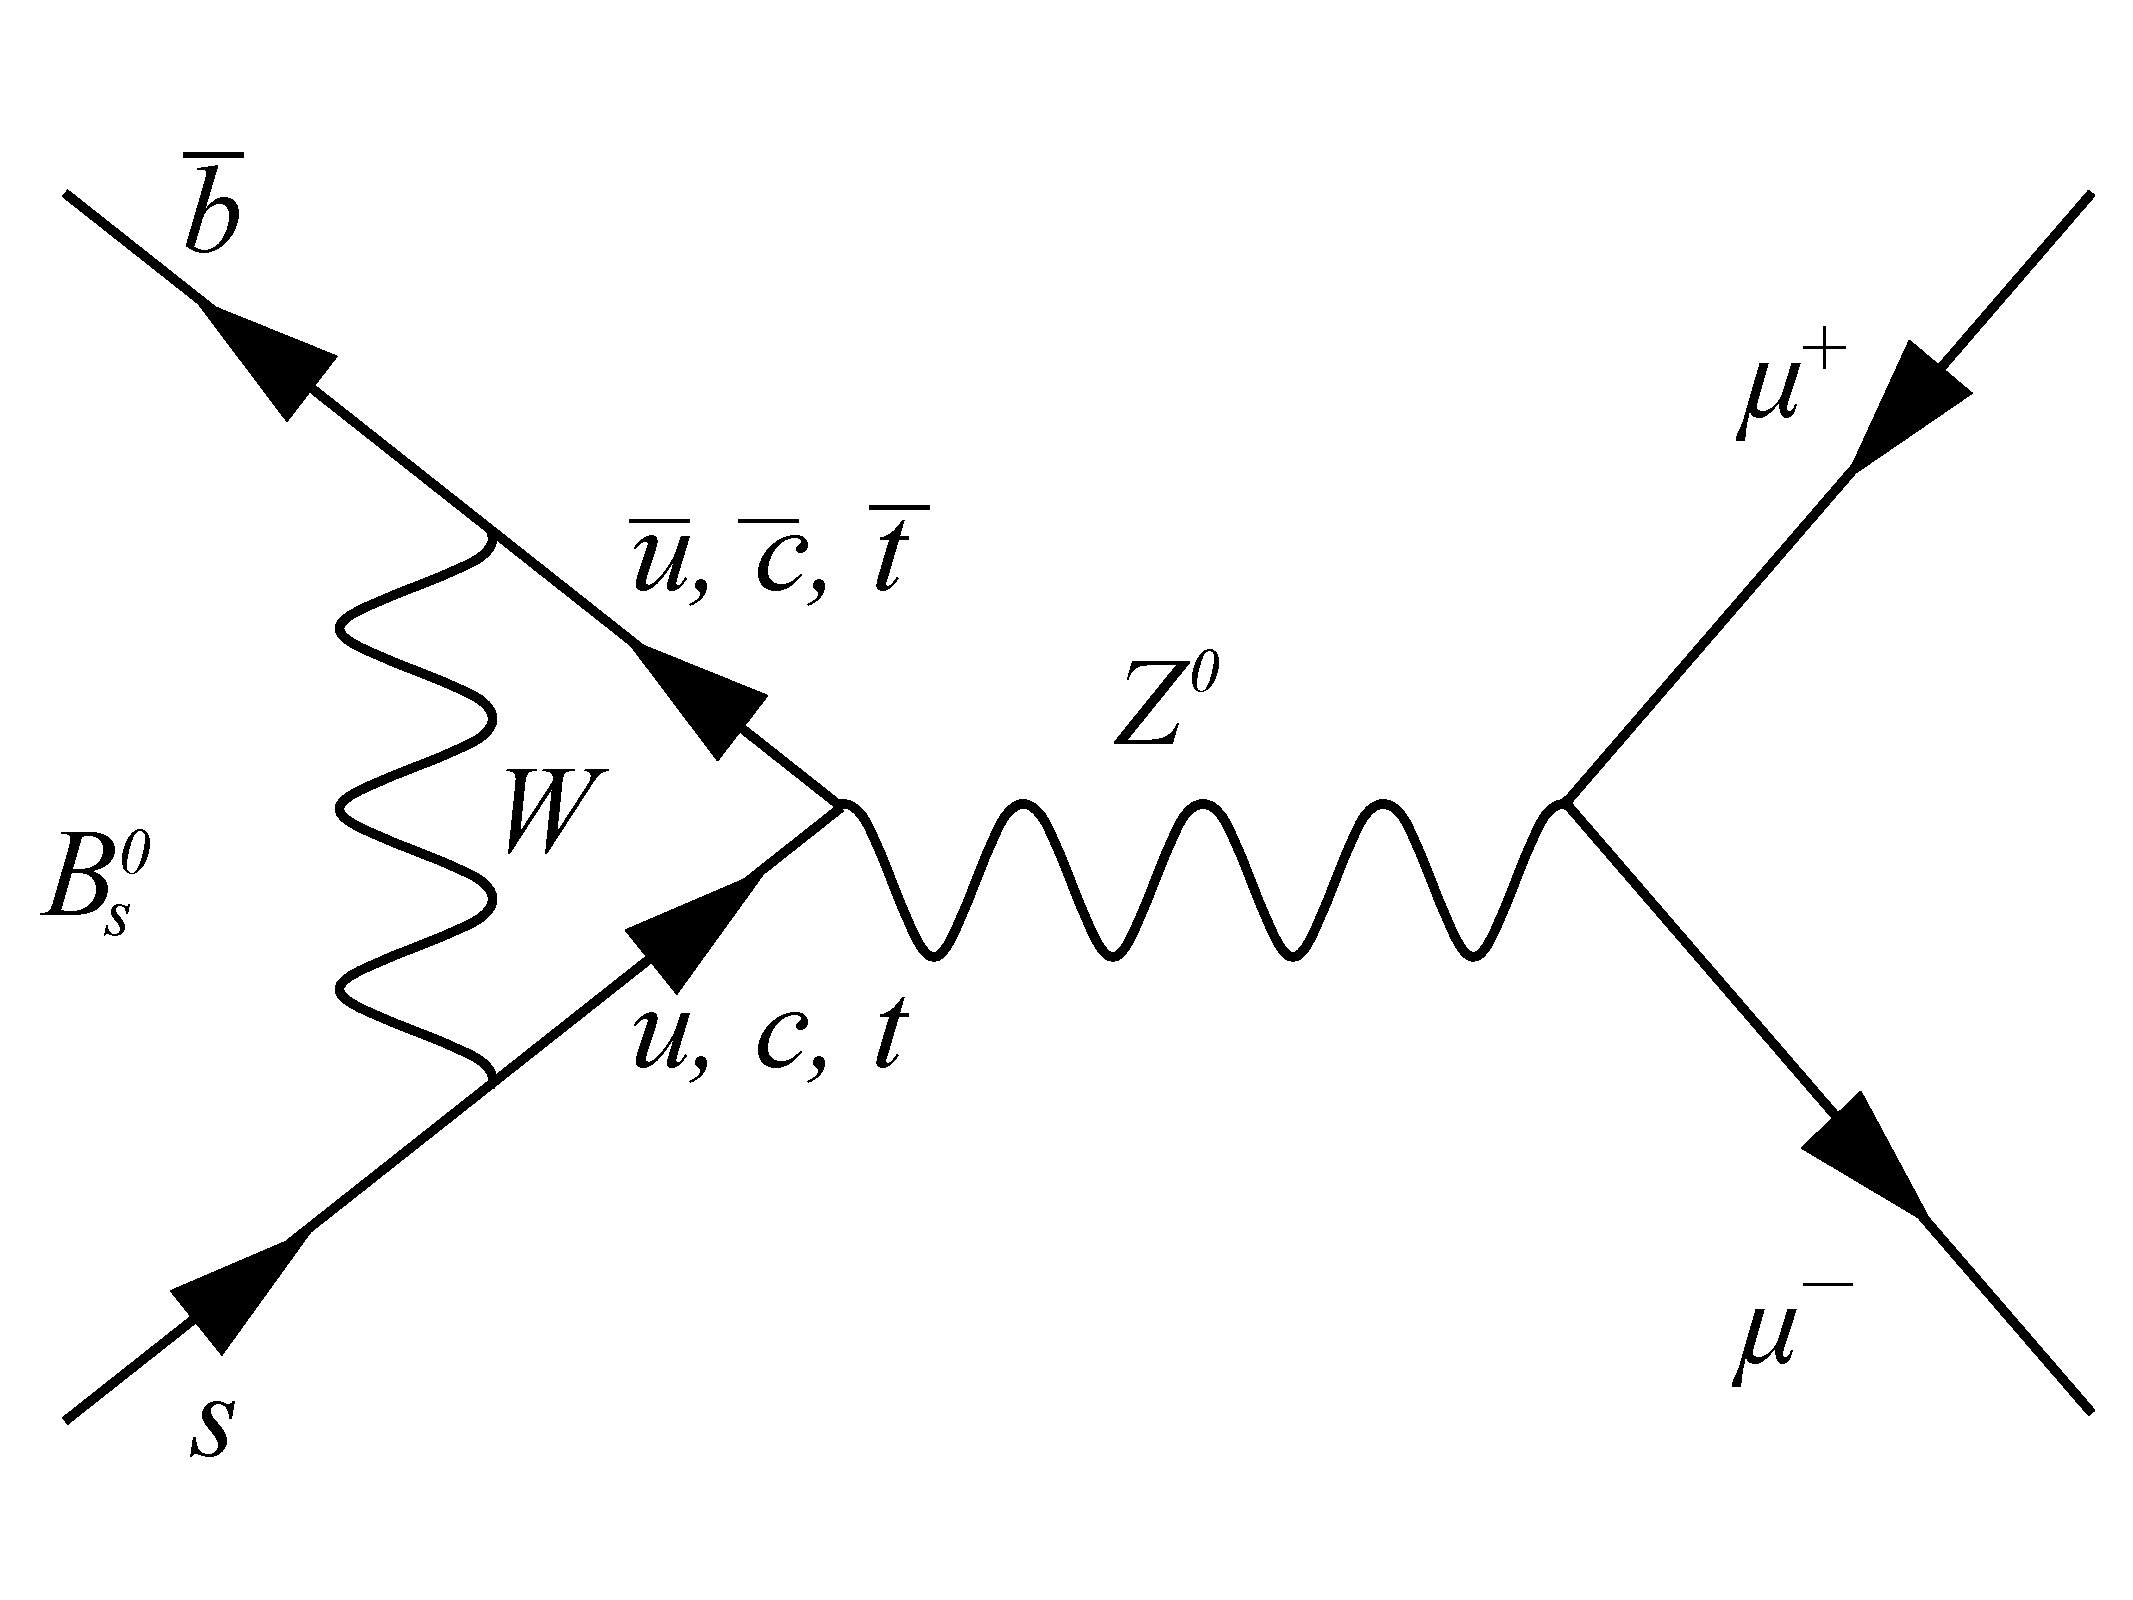
\includegraphics[width=0.4\textwidth]{./Figs/Theory/Z0_penguin_v2.pdf}
    \caption{Feynman diagrams for \bsmumu decays in the SM via $W$-box and $Z^0$-penguin processes. The same diagrams apply to \bdmumu decays but the $s$ quark is exchanged for a $d$ quark.}
    \label{fig:SM_diag}
\end{figure}

The decays can also proceed via Higgs-penguin diagrams however the contributions from these diagrams are negligible. %within the SM.
The lack of \bmumu decays at the tree level causes them to be suppressed compared to other \bsd decay modes that can occur at the tree level.

%{\it I think that this needs to be re-worded.

%Although the weak force allows quark flavour to change the coupling strengths between different quark flavours are not all the same magnitude. The coupling strengths are described by the CKM matrix. Quarks can Quarks fall into three families; $u$ and $d$, $c$ and $s$, $t$, and $b$. They can also be separated into two types depending on their charge; up-type quarks include $u$, $c$ and $t$, down-type quarks include $d$, $s$ and $b$. The weak force couples up-type quarks to the weak eigenstates of the down-type quark in the same family with the same strength. The weak quark eigenstates are not the same as the mass eigenstates and the two types of states are related via the CKM matrix as
%}

%{\it where $d^', s^'$ and $b^'$ are weak eigenstates and $d, s$ and $b$ are mass eigenstates. The CKM matrix is a unitary matrix, which ensures no tree level FCNCs occur, with complex elements that give the coupling strengths of different quarks, for example the amplitude of a $u$ quark changing into a $d$ quark is proportional to $|V_{ud}|$.}


Although the weak force allows quark flavour to change the coupling strengths between different quark flavours are not all the same magnitude. The coupling strengths are described by the CKM matrix. Quarks can be separated into two types depending on their charge; up-type quarks include $u$, $c$ and $t$, down-type quarks include $d$, $s$ and $b$. The weak force couples all up-type quarks to the weak eigenstate of the down-type quark in the same family with the same strength. Where the quark families are; $u$ and $d$, $c$ and $s$, $t$, and $b$. The weak quark eigenstates are not the same as the mass eigenstates and the two types of states are related via the CKM matrix~\cite{PhysRevLett.10.531,doi:10.1143/PTP.49.652} as
\begin{equation}
\begin{pmatrix}
d'\\
s'\\
b'
\end{pmatrix}
= 
\mathbf{V_{CKM}}
\begin{pmatrix}
d\\
s\\
b
\end{pmatrix} =
 \begin{pmatrix}
   V_{ud} & V_{us} & V_{ub} \\
   V_{cd} & V_{cs} & V_{cb} \\
   V_{td} & V_{ts} & V_{tb}
 \end{pmatrix}
\begin{pmatrix}
d\\
s\\
b
\end{pmatrix}
\label{eq:CKMA}
\end{equation}
where $d'$, $s'$ and $b'$ are weak eigenstates and $d$, $s$ and $b$ are mass eigenstates. The CKM matrix is a unitary matrix with complex elements which ensures no tree level FCNCs occur. Each element of the matrix gives the coupling strengths of transitions between the mass eigenstates of quarks, for example the amplitude of a $u$ quark changing into a $d$ quark is proportional to $|V_{ud}|$.

The difference in the coupling strength sizes can illustrated through the Wolfenstein parametrisation of the CKM matrix~\cite{PhysRevLett.51.1945}, which parametrises the matrix elements in powers of the small parameter of $\lambda = 0.22 \approx |V_{us}|$. The CKM matrix then becomes
\begin{equation}
\mathbf{V_{CKM}} =
 \begin{pmatrix}
 1 - \frac{1}{2}\lambda^2 & \lambda & \lambda^3 A (\rho - i \eta) \\
 - \lambda                & 1 - \frac{1}{2}\lambda^2 & \lambda^2 A \\
 \lambda^3 A (1 - \rho- i \eta) & -\lambda^2 A & 1
 \end{pmatrix} + \mathcal{O}(\lambda^4).
\label{eq:CKMB}
\end{equation}
This parametrisation shows that the CKM matrix is almost diagonal. For a \bmumu decay to occur one off diagonal element in needed to described the quark transitions in Figure~\ref{fig:SM_diag}. Therefore introducing an additional source of suppression to the decay. 

The internal quark lines in Figure~\ref{fig:SM_diag} can have contributions from $u$, $c$ and $t$ quarks. However in the SM the contributions from $u$ and $c$ quarks are negligible when compared to the $t$ quark. This is due to the large $t$ quark mass and because the coupling strength of the $b$ quark to any quark except the $t$ is extremely small.


The final source of suppression of \bmumu decays comes from the helicities of the muons in the final state. Both \bd and \bs are spin zero particles and for angular momentum to be conserved in the decay the spins of the two muons must be oppositely aligned. This leads to the muons having opposite helicities. % Therefore the production of one of the muons will always be suppressed.
The weak force only couples to left-handed particle states and right-handed anti-particle states. In the high energy limit where particles are massless, negative helicity states are equal to left-handed states and positive helicity states are equal to right-handed states.
Therefore if the muons were massless the weak interaction could only produce a $\mu^-$ and a $\mu^+$ with opposite helicities which cannot conserve angular momentum in \bmumu decays.
Muon are not massless therefore \bmumu decay can occur but are suppressed because $m_{\mu} \ll M_{B_{(s)}$~\cite{Olive:2016xmw} leading to one of the helicity states of the muons always being disfavoured.

Overall \bmumu decays are highly suppressed within the framework of the SM compared to other decay modes of \bsd mesons. Therefore these decays offer excellent processes in which to search for NP because the contribution of BSM theories to these decay rates can be at a similar order of magnitude to those from the SM.

\section[\bmumu Branching Fraction]{\boldmath{\bmumu} Branching Fraction}
\label{sec:BFdef}
The \BF of a particle decay offers an excellent observable through which predictions of the SM can be compared to measured values. The \bmumu \BF is defined as the fraction of the total number of \bsd particles that decay into two muons. It can be calculated from the decay rate, which is the probability per unit time that a \bsd decays into two muons, as
\begin{equation}
\mathcal{B}(B^0_{(s)} \to \mu^+ \mu^-) \equiv \frac{\Gamma(B^0_{(s)}(t) \to \mu^+ \mu^-) + \Gamma(\
\overline{B}^0_{(s)}(t) \to \mu^+ \mu^-)}{\Gamma(B^{0}_{(s)}) + \Gamma(\overline{B}^{0}_{(s)}) }
\end{equation}

The SM predictions are calculated from the `prompt' decay rate that ignore any evolution with time of the \bsd particles. The \BFs are calculated using~\cite{DeBruyn:2012wj} 
\begin{equation}
\mathcal{B}(B^0_{(s)} \to \mu^+ \mu^-)_{\mathrm{th}} = \frac{ \tau_{B_{(s)}} }{2} \langle \Gamma(B^0_{(s)}(t) \to \mu^+ \mu^-) \rangle \big{|}_{t=0}
\label{sec:BF_prompt}
\end{equation}
where $\tau_{B_{(s)}$ is the mean lifetime of the \bsd and $\langle \Gamma(B^0_{(s)}(t) \to \mu^+ \mu^-) \rangle$ is defined as
\begin{equation}
\langle \Gamma(B^0_{(s)}(t) \to \mu^+ \mu^-) \rangle = \Gamma(B^0_{(s)}(t) \to \mu^+ \mu^-) + \Gamma(\overline{B}^0_{(s)}(t) \to \mu^+ \mu^-).
\end{equation}
The \BFs are calculated this way to enable easy comparison of different $B$ meson \BFs including \bd, \bs and $B^+$~\cite{DeBruyn:2012wj}.

The prompt decay rate is evaluated from Fermi's golden rule, relating the decay rate  to the transition amplitude, $\left|\mathcal{M}(B^0_{(s)} \to \mu^+ \mu^-)\right|$, and the kinematics of the decay to give~\cite{Tolk:2148631}
\begin{equation}
\Gamma(B^0_{(s)}(t) \to \mu^+ \mu^-)\big{|}_{t=0} = \frac{1}{16\pi} \frac{1}{M_{B_{(s)}}} \sqrt{1 -4 \left (\frac{m_{\mu}}{M_{B_{(s)}}} \right )^2} \left|\mathcal{M}(B^0_{(s)} \to \mu^+ \mu^-)\right|^2
\label{sec:FGR}
\end{equation}
where $m_{\mu}$ and $M_{B_{(s)}}$ are the masses of the muon and the \bsd, respectively. The factor of $\right( \frac{m_{\mu}}{M_{B_{(s)}}}\left)$ comes from the helicity suppression discussed in Section~\ref{sec:bsmumu_in_SM}.


Weak decays like \bmumu include interactions that occur at different energy scales, from the weak propagators at $M_W \approx 80$~\gevcc to the strong coupling in the \bsd meson at $\Lambda_{QCD} \sim 0.2$~\gev~\cite{Olive:2016xmw}. %This enable the Operator Product Expansion~\cite{} method to be used to construct the effective Hamiltonian, $\mathcal{H}_{eff}$, and calculate the transition amplitude $|\matcal{M}(B^0_{(s)} \to \mu^+ \mu^-)| = \langle \mu \mu | \mathcal{H}_{eff} | B^0_{(s)} \rangle$. The effective Hamiltonian divides the interaction into two energy levels with the structure
The Operator Product Expansion~\cite{PhysRev.179.1499,Wilson1972} is used to create the effective hamiltonian, $\mathcal{H}_{eff}$, which splits the interaction into two energy levels. The transition amplitude then becomes 
\begin{equation}
|\matcal{M}(B^0_{(s)} \to \mu^+ \mu^-)| \equiv \langle \mu \mu | \mathcal{H}_{eff} | B^0_{(s)} \rangle  = \frac{G_F}{\sqrt{2}} \displaystyle\sum_{i} V^i_{CKM} \langle \mu \mu | \mathcal{C}(\mu)_i \mathcal{O}(\mu)_i | B^0_{(s)} \rangle
\label{sec:eff_hamil_def}
\end{equation}
where $G_F$ is the Fermi coupling constant, $V_{CKM}^i$ are CKM matrix elements, $\matcal{C}_i$ are Wilson coefficients and $\mathcal{O}_i$ are local operators. The energy scale $\mu$ separates the two energy levels in the interaction. The Wilson coefficients describe short scale processes with energies above $\mu$. This incorporates the internal structure and loops of Feynman diagrams leading to the dependance of Wilson coefficients on the $W^{\pm}$, $Z^0$, $H^0$ and $t$ quark masses. The long distance processes are described by the local operators $\mathcal{O}_i$ for energies less than $\mu$. The local operators link the initial and final states of the decay. % indendant of the internal structure of the interaction. 
Wilson coefficients can be calculated using perturbation theory however this cannot be used for the local operators which can lead to large theoretical uncertainties on their values. The choice of $\mu$ is arbitrary however the final transition amplitude must be independent of $\mu$, often the mass of the decaying particle is used. 

%The Operator Product Expansion can be used to describe weak decays with different initial and final states as well as internal structure. 
In the effective Hamiltonian in Equation~\ref{sec:eff_hamil_def} the CKM matrix elements are factored out of the Wilson coefficients and operators, therefore the same coefficients and operators can be used to describe the \bd and \bs decays.
The effective Hamiltonian for \bmumu decays is~\cite{DeBruyn:2012wk}
\begin{equation}
\mathcal{H}_{eff} = -\frac{G_F \alpha}{\sqrt{2\pi}} V_{tq}^{*}V_{tb} \displaystyle\sum_{i}^{10,S,P} (\matcal{C}_i\matcal{O}_i + \matcal{C}^{'}_{i}\matcal{O}_{i}^{'})
\label{eq:eff_hamil_bmumu}
\end{equation}
where $\alpha$ is the fine structure constant and $q$ corresponds to the $d$ quark in the \bd or the $s$ quark in the \bs. Terms proportional to $V^*_{cq}V_{cb}$ and $V^*_{cq}V_{ub}$ neglected because they are negligible. The operators that can contribute to the \bmumu effective Hamiltonian due to the initial and final decay states are
\begin{align}
 \mathcal{Q}_{10}&=(\bar{q}\gamma^{\mu}P_{L}b)(\bar{l}\gamma_{\mu}\gamma_{5}l), &\qquad
 \mathcal{Q}_{10}^{(')}&= (\bar{q}\gamma^{\mu}P_{R}b)(\bar{l}\gamma_{\mu}\gamma_{5}l), \\
 \mathcal{Q}_{S}&= m_{b}(\bar{q}P_{R}b)(\bar{l}l),  &\qquad
\mathcal{Q}_{S}^{(')}&= m_{b}(\bar{q}P_{L}b)(\bar{l}l), \\
 \mathcal{Q}_{P}&= m_{b}(\bar{q}P_{R}b)(\bar{l}\gamma_{5}l), &\qquad
 \mathcal{Q}_{P}^{(')}&= m_{b}(\bar{q}P_{L}b)(\bar{l}\gamma_{5}l).
\end{align}
%\begin{eqnarray}
% \mathcal{Q}_{10}&=(\bar{q}\gamma^{\mu}P_{L}b)(\bar{l}\gamma_{\mu}\gamma_{5}l),  \qquad
% \mathcal{Q}_{10}^{(')}&= (\bar{q}\gamma^{\mu}P_{R}b)(\bar{l}\gamma_{\mu}\gamma_{5}l), \\
% \mathcal{Q}_{S}&= m_{b}(\bar{q}P_{R}b)(\bar{l}l),  \qquad
%\mathcal{Q}_{S}^{(')}&= m_{b}(\bar{q}P_{L}b)(\bar{l}l), \\
% \mathcal{Q}_{P}&= m_{b}(\bar{q}P_{R}b)(\bar{l}\gamma_{5}l),  \qquad
% \mathcal{Q}_{P}^{(')}&= m_{b}(\bar{q}P_{L}b)(\bar{l}\gamma_{5}l) 
%\label{eq:operators}
%\end{eqnarray}
The operator $\mathcal{O}_{10}$ encompasses the only significant contributions in the SM that come from $W$-box and $Z^0$ penguin diagrams. The operator $\mathcal{O}_{10}^'$ describes the equivalent interactions as $\mathcal{O}_{10}$ but for right handed currents that are forbidden in the SM. %, de and $\mathcal{O}_{10}^'$ does not contribute in the SM because is describes right handed currents.% which are forbidden in weak interactions in the SM are described by $\mathcal{O}_{10}^'$ and 
 Finally, the operators $\mathcal{O}_{S}^{(')}$ and $\mathcal{O}_{P}^{(')}$ correspond to the exchange of scalar and pseudo-scalar particles which is negligible in the SM. 

The purely leptonic final state of \bmumu decays means that the computation of the transition amplitude can be spilt in two so that all uncertainties arising from the bound \bsd states are encompassed into one parameter, $F_{B_{(s)}}}$, the hadronic decay factor. This leads to a theoretically clean prediction for the \BF.

The \BFs for \bmumu decays can therefore be written as~\cite{Buras:2013uqa}
\begin{equation}
\mathcal{B}(B^{0}_{(s)} \to \mu^{+} \mu^{-})=&\frac{\tau_{B_{(s)}}G_{F}^{4} M_{W}^{4} \sin^{4}\theta_{W} }{8\pi^{5}} \big|\mathcal{C}_{10}^{SM} V^{*}_{tq}V_{tb}\big|^{2} F_{B_{(s)}}M_{B_{(s)}} m_{\mu}^{2} \sqrt{1 - \frac{4m_{\mu}^{2}}{M^{2}_{B_{(s)}}}} (|P|^{2} + |S|^{2})
\label{eq:BF_form}
\end{equation}
where $\theta_W$ is the weak mixing angle and $M_{W}$ the mass of the $W$ boson. The \BF has been parametrised in terms of $\mathcal{C}_{10}^{SM}$, $P$ and $S$, where $\mathcal{C}_{10}^{SM}$ is the SM value of the operator $\mathcal{C}_{10}$ and 
\begin{equation}
P \equiv |P| e^{i\varphi_P} \equiv \frac{\mathcal{C}_{10} - \mathcal{C}_{10}^{'}}{\mathcal{C}_{10}^{SM}} + \frac{M^2_{B_{(s)}}}{2m_{\mu}} \frac{m_b}{m_b + m_q} \frac{\mathcal{C}_{P} - \mathcal{C}_{P}^{'}}{\mathcal{C}_{10}^{SM}} 
\label{eq:P}
\end{equation}
\begin{equation}
S \equiv |S| e^{i\varphi_S} \equiv \sqrt{1- \frac{4m_{\mu}^{2}}{M^{2}_{B_{(s)}}}} \frac{M^{2}_{B_{(s)}}}{2m_{\mu}}  \frac{m_b}{m_b + m_q}  \frac{\mathcal{C}_{S} - \mathcal{C}_{S}^{'}}{\mathcal{C}_{10}^{SM}} 
\label{eq:S}
\end{equation}
In the SM $P=1$ and $S=0$, however the \BFs are parametrised in terms of $P$ and $S$ because BSM theories can significantly alter their values. 
%The dependence of the \BFs on $\mathcal{C}_{10}$ makes \bmumu decays one of the best decays to study this parameter and these decays are also very sensitive to scale particles~\cite{}. 
The presence of scalar particles could increase the \BFs above the SM expectation through $\mathcal{C}_S^{(')}$ leading to $S>0$, also the contributions from scalar particles are not subject to helicity constraints. Pseudoscalar particles can either enhance or suppress the \BFs compared to the SM prediction depending on how the values of $\mathcal{C}_P^{(')}$ interfere with $\mathcal{C}_{10}^{(')}$ in NP models.


As well as the individual \BFs of \bdmumu and \bsmumu decays the ratio of the two \BFs is also an interesting observable. The ratio of \BFs is given by
\begin{equation}
  \mathcal{R} = \frac{\mathcal{B}(B^{0} \to \mu^{+} \mu^{-})}{\mathcal{B}(B^{0}_{s}\to \mu^{+} \mu^{-})} = \frac{\tau_{B}}{\tau_{B_{s}}} \bigg{|} \frac{V_{td}}{V_{ts}} \bigg{|}^{2} \frac{M_{B}^{2}}{M_{B_{s}}^{2}} \sqrt{\frac{1 - \frac{4m_{\mu}^{2}}{M^{2}_{B}}}{1- \frac{4m_{\mu}^{2}}{M^{2}_{B_{s}}}}} 
\label{eq:BF_ratio}
\end{equation}
and the uncertainty on the ratio is less that the individual \BFs because sources of uncertainties including those from Wilson coefficients and $|V_{tb}|$ cancel out. The ratio does not depend on Wilson coefficients and provides an excellent observable to test the flavour structure of the SM and BSM theories.


\section{Quark mixing}
\label{sec:quarkmaixing}
The theoretical prediction for the \bmumu \BFs does not take into account the evolution of the \bsd and \barbsd mesons with time. Once a \bsd is created it will oscillate between the particle and anti-particle states as it propagates through time, the same is true for the \barbsd. Therefore the states that travel through time are a superposition of the \bsd and the \barbsd. These oscillation occurs as the constituents quarks transition between different flavours through the exchange of $W$ bosons as illustrated in Figure~\ref{fig:Oscl_diag}.
\begin{figure}[htbp]
    \centering
        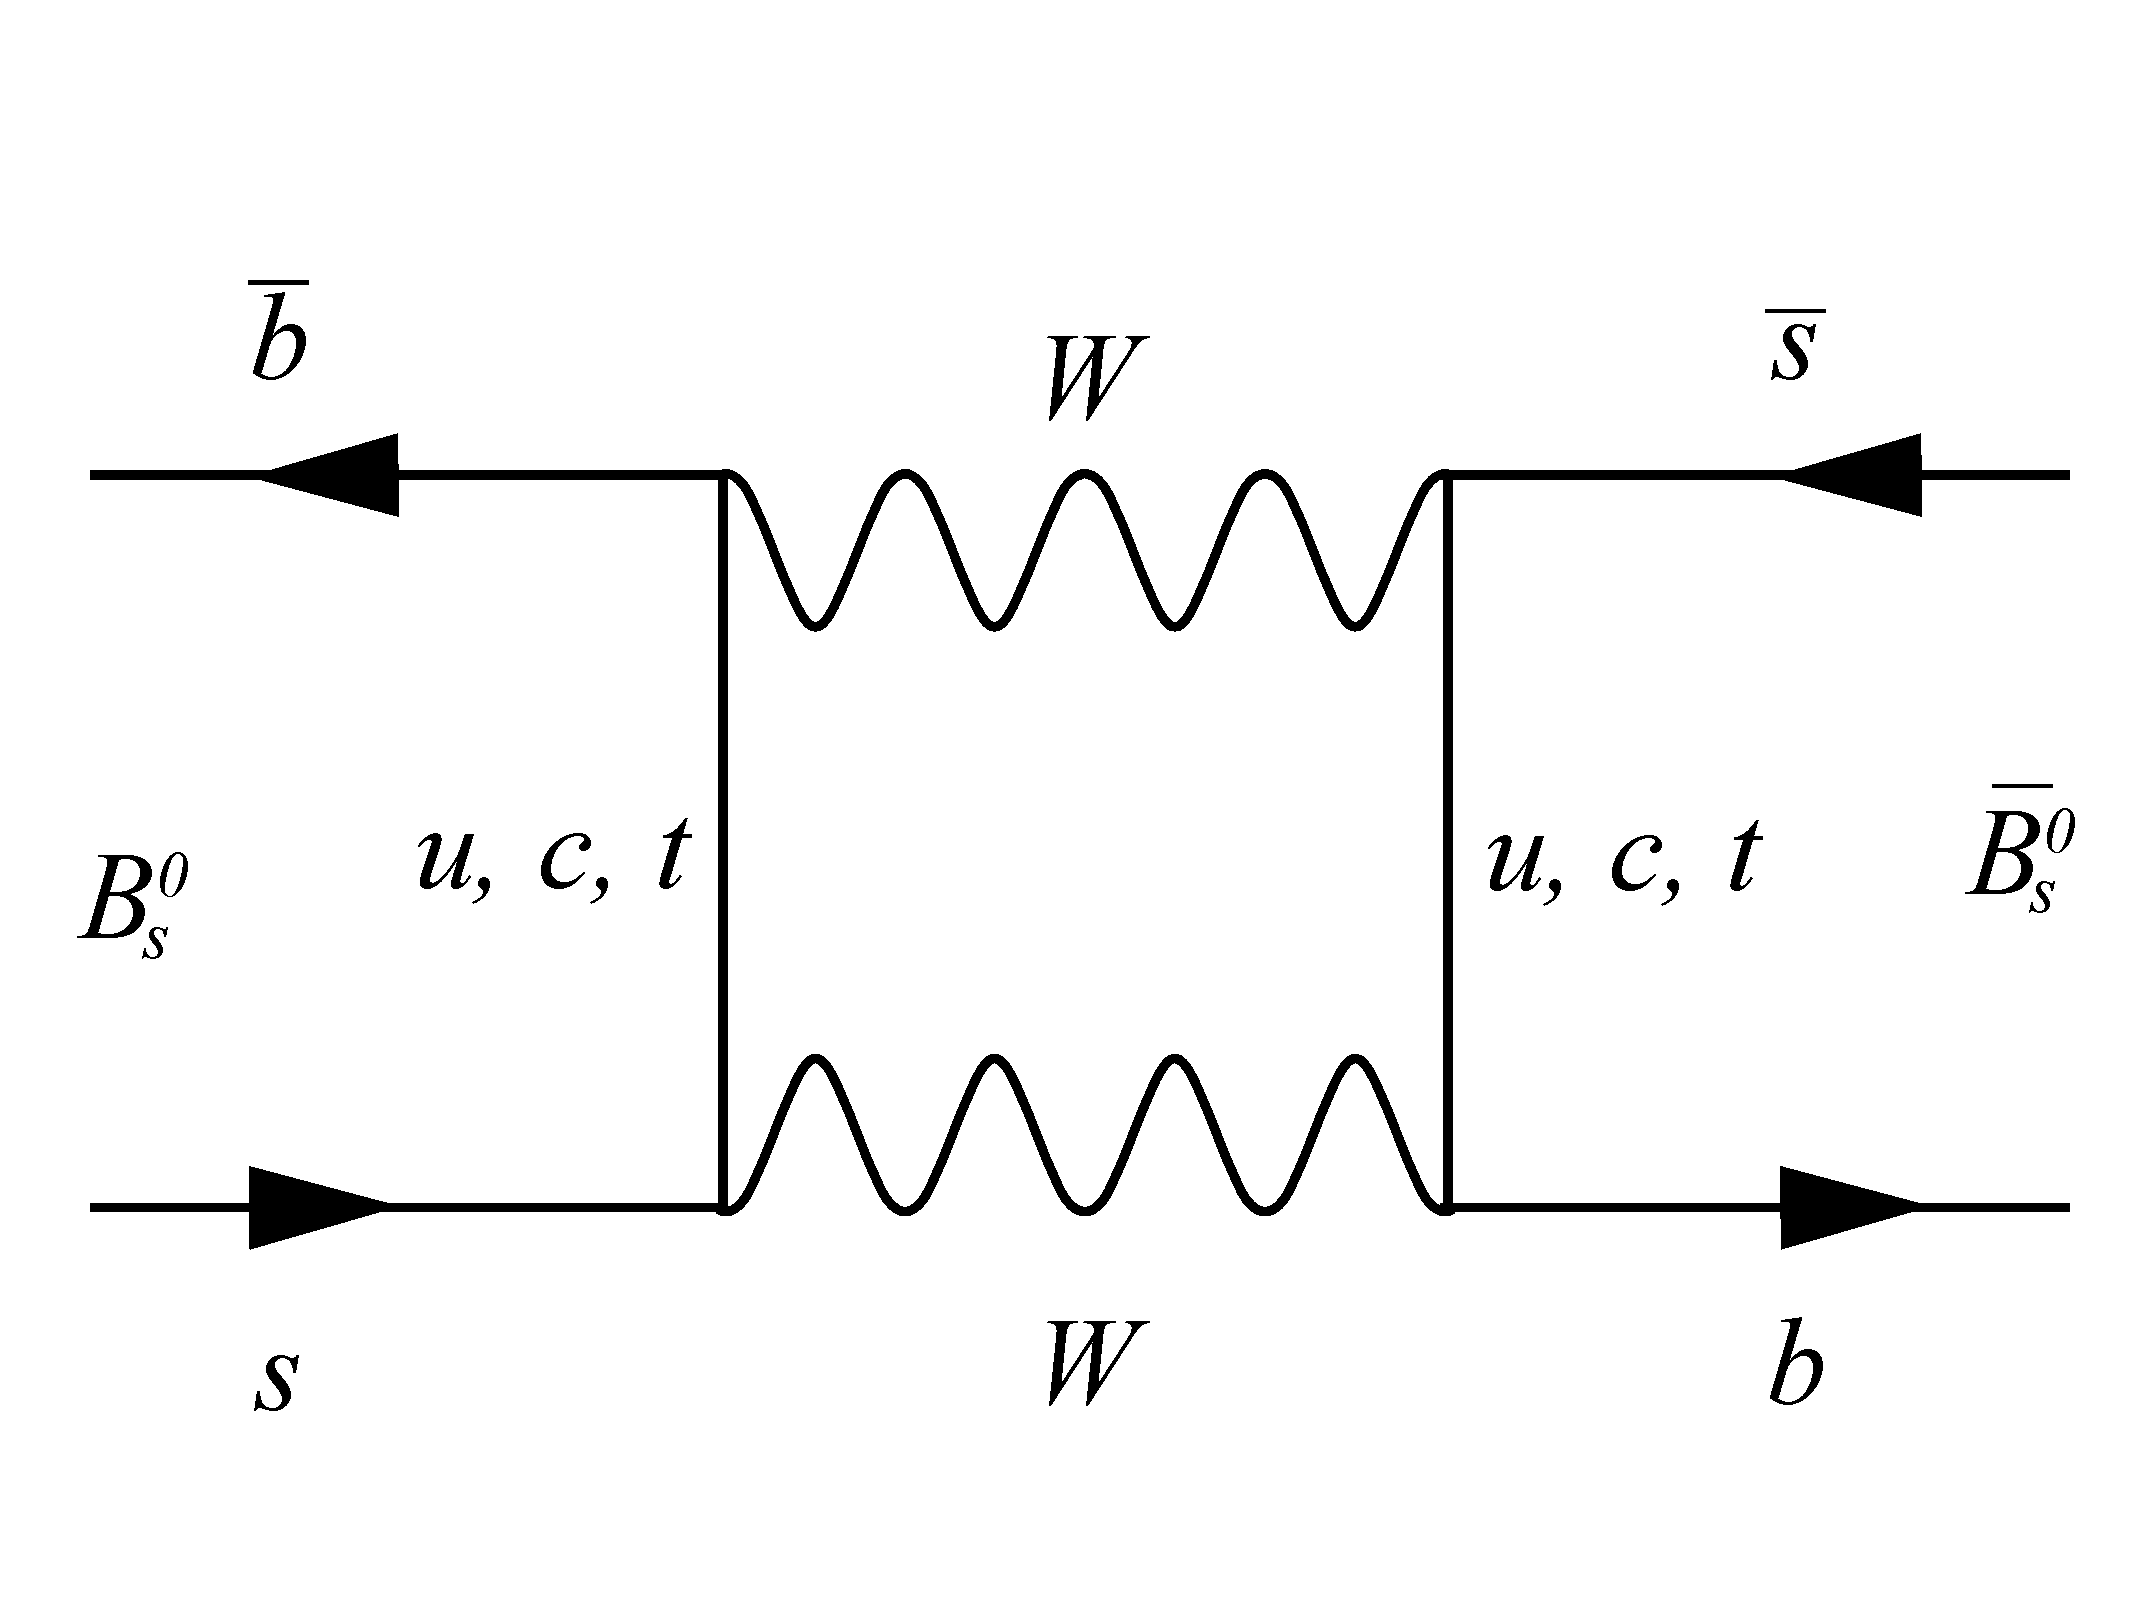
\includegraphics[width=0.5\textwidth]{./Figs/Theory/Oscillation_1.pdf}
        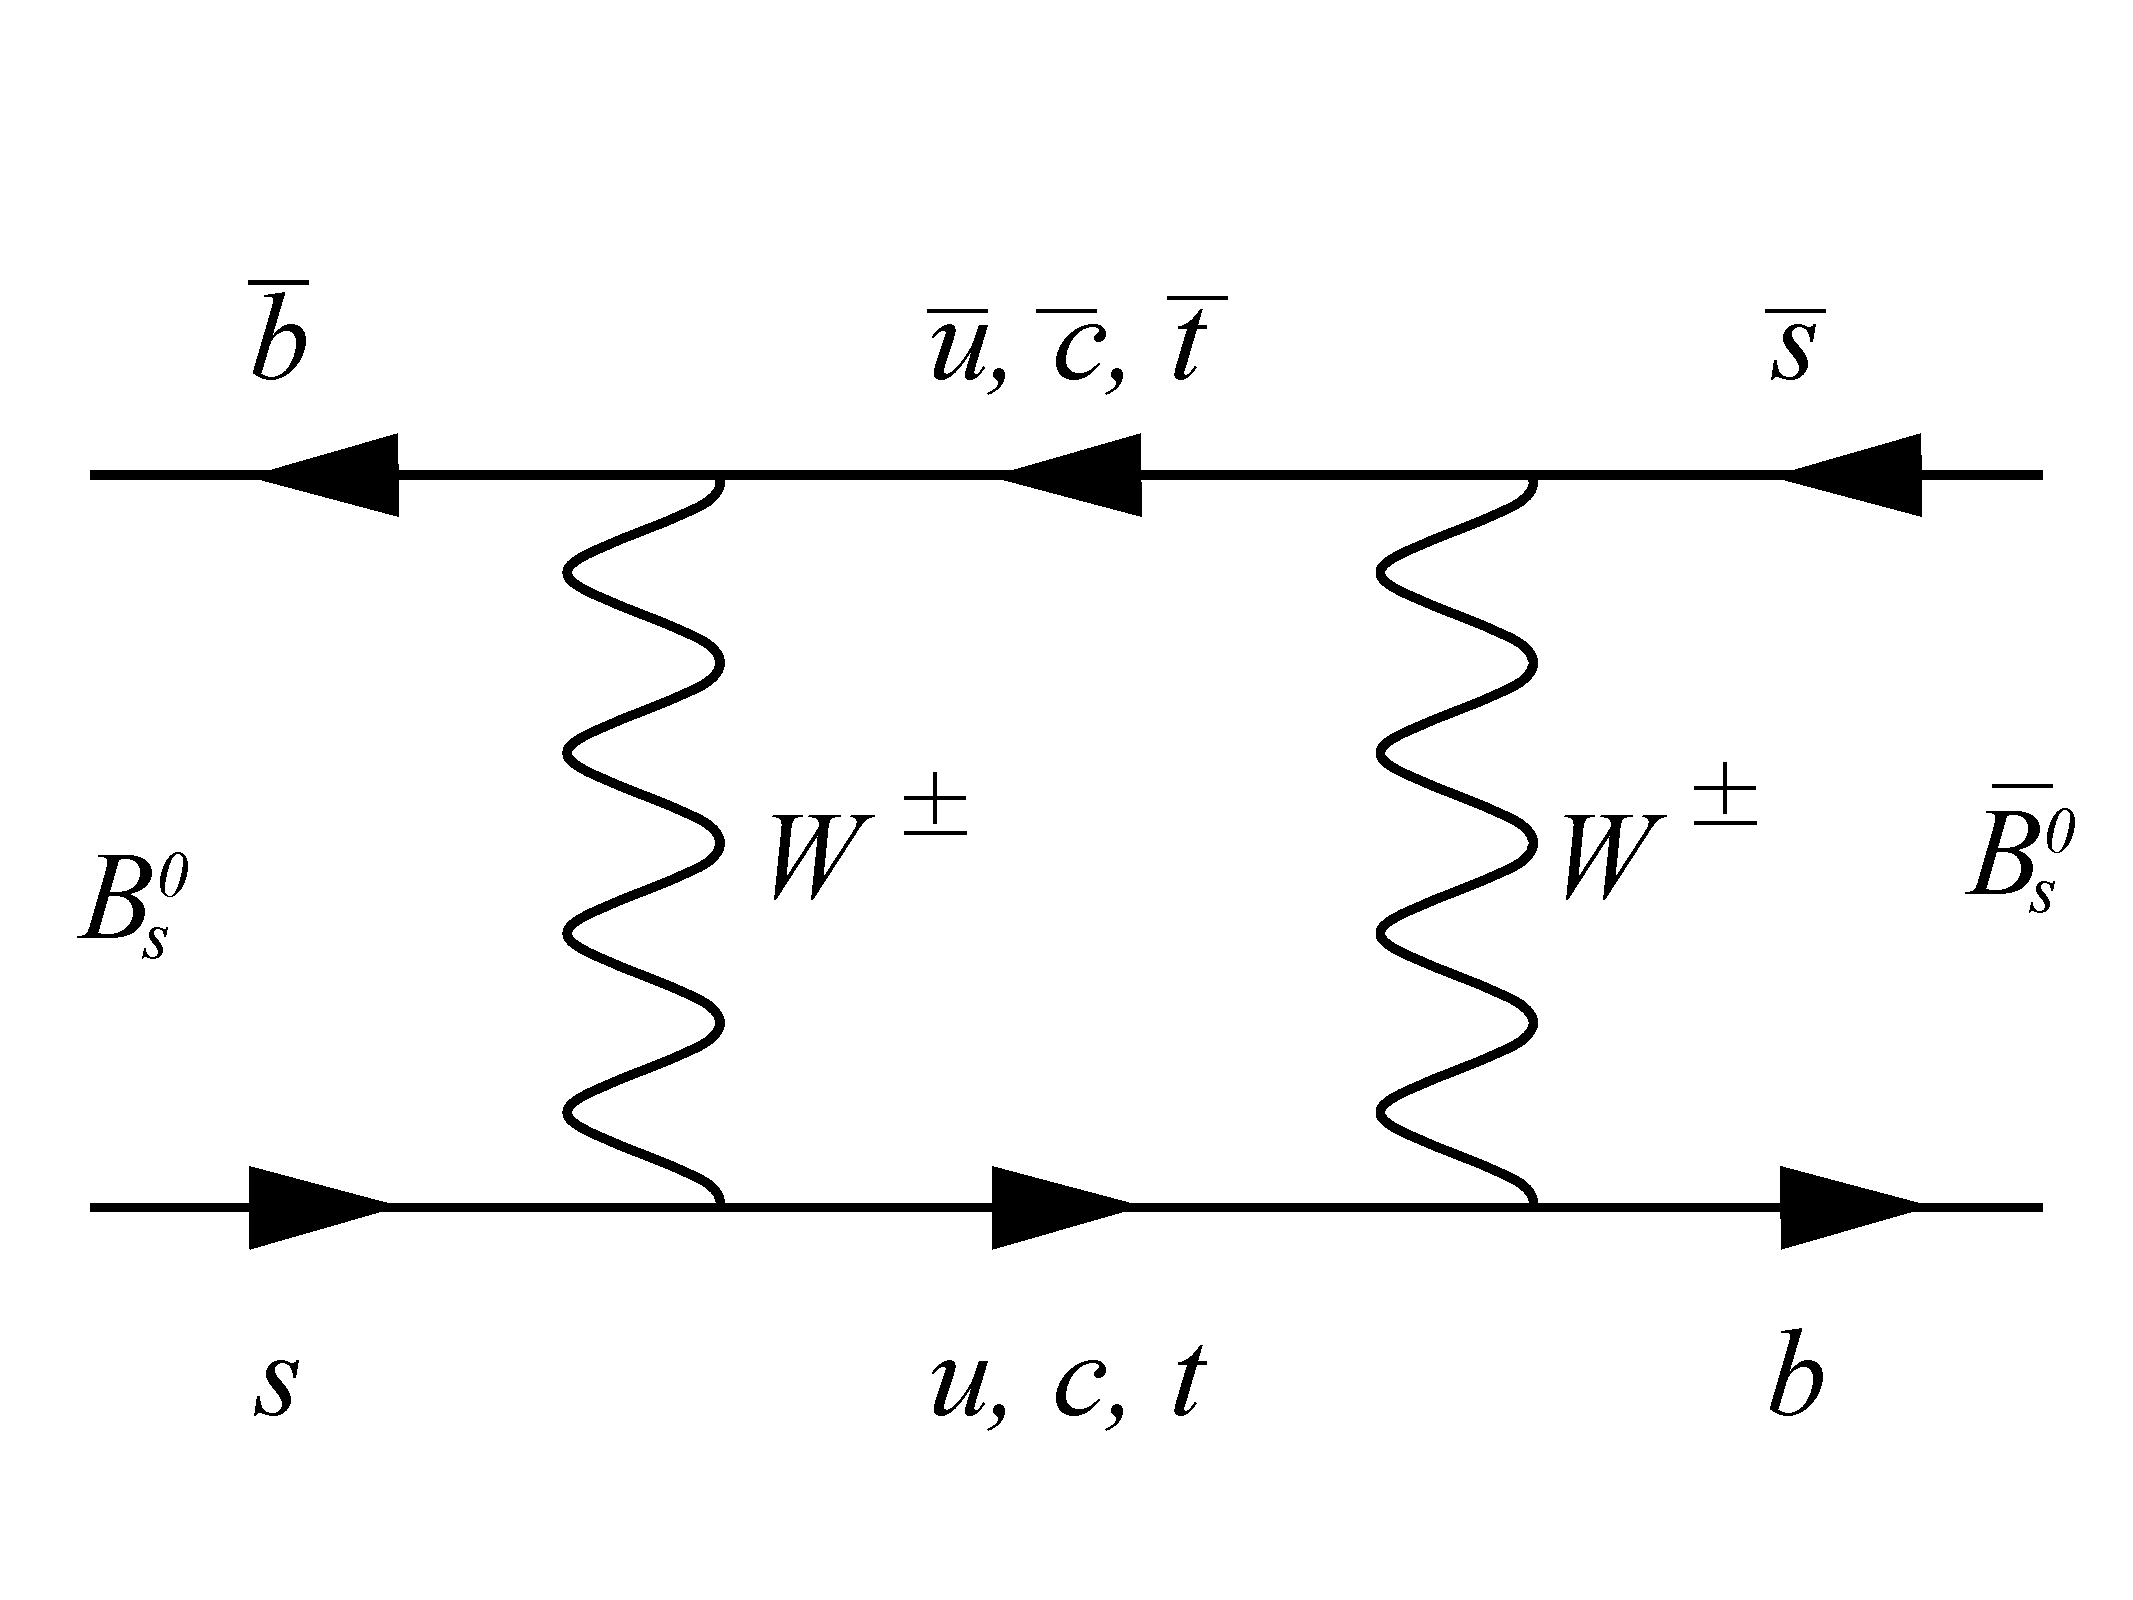
\includegraphics[width=0.5\textwidth]{./Figs/Theory/Oscillation_2.pdf}
    \caption{Oscillation of \bs and \barbs quarks through the exchange of $W$ bosons. The same diagrams apply to \bd and \barbd oscillations but with the $s$ quark exchanged for a $d$ quark.}
    \label{fig:Oscl_diag}
\end{figure}
The \BFs are measured from data where \bsd and \barbsd decays are not separated, which is called as an untagged sample of \bmumu decays. Since a \bsd or \barbsd lives for $\sim 10^{-12}$~s before decaying the state that decays will not necessarily be the same as the one that was produced. The measured \BF is not the same as the `prompt' \BF used for the theoretical prediction, the measured value corresponds to the time integrated \BF given by~\cite{DeBruyn:2012wj}
\begin{equation}
  \mathcal{B}(B^0_{(s)} \to \mu^+ \mu^-)_{\mathrm{exp}} \equiv \frac{1}{2} \int^{\infty}_0 \langle \Gamma(B^0_{(s)}(t) \to \mu^+\mu^-) \rangle dt.
\label{eq:time_BF}
\end{equation}
Therefore for a meaningful comparison between the measured and predicted \BF values, the difference in the two definitions must be evaluated~\cite{DeBruyn:2012wk,Buras:2013uqa,DeBruyn:2012wj}.

\subsection[Time evolution of the \bsd]{Time evolution of the \boldmath{\bsd}}
\label{sec:oscillations}
Initially each $b$ and $\bar{b}$ quark hardonises to form a \bsd or \barbsd described at $t=0$ by the states $| B^0_{(s)} \rangle$ and $| \overline{B}^0_{(s)} \rangle$. In order to evaluate the time integrated \BFs the evolution of these states with time must be evaluated. The time dependant Schr\"{o}dinger equation (TDSE) describes the time evolution of the particle and anti-particle states as
\begin{equation}
i \frac{d}{dt}\begin{pmatrix}{| B^0_{(s)}(t) \rangle \\ | \overline{B}^0_{(s)}(t) \rangle }\end{pmatrix} = \Bigg{(} \mathbf{M} - \frac{i\mathbf{\Gamma}}{2} \Bigg{)} \begin{pmatrix}{| B^0_{(s)}(t) \rangle \\ | \overline{B}^0_{(s)}(t) \rangle }\end{pmatrix}. 
\label{eq:TDSE}
\end{equation}
$\mathbf{M}$ and $\mathbf{\Gamma}$ are $2 \times 2$ hermitian matrices describing mass and decay time with the properties $M_{12}^{*} = M_{21}$ and $\Gamma_{12}^{*} = \Gamma_{21}$. Invariance under charge, parity and time inversion introduces additional constraints of $M_{11} = M_{22}$ and $\Gamma_{11} = \Gamma_{22}$. 

The \bsd-\barbsd oscillations ensure that for any $t>0$ the particles are a superposition of $| B^0_{(s)} \rangle$ and $| \overline{B}^0_{(s)} \rangle$ states. The off diagonal elements in the mass and decay time matrices mean that the eigenstates of the TDSE have different masses and lifetime to the \bsd and \barbsd. The eigenstates can be given by heavy, $H$, and light, $L$, mass states defined at $t=0$ as
\begin{equation}
| B_H \rangle = p | B^0_{(s)} \rangle - q |\overline{B}^0_{(s)} \rangle, \qquad |B_L \rangle = p  | B^0_{(s)} \rangle + q \overline{B}^0_{(s)} \rangle
\label{eq:mass_states}
\end{equation}
with eigenvalues of $(m_{H,L} - i\Gamma_{H,L}/2)$ and the coefficients $p$ and $q$ are constrained by $|p|^2 + |q|^2 = 1$. The eigenvalues are different for the \bd and \bs systems however the treatment of the two systems is identical, to simplify the notation only the \bs system will be described in the following discussion.
The time evolution of the heavy and light mass eigenstates is given by
\begin{equation}
  | B_H (t)\rangle = | B_H \rangle e^{-i(m_H - i\frac{\Gamma_H}{2})t}, \qquad | B_L (t)\rangle = | B_L \rangle e^{-i(m_L - i\frac{\Gamma_L}{2})t}
\label{eq:time1}
\end{equation}
from the TDSE. Therefore the time evolution of the flavour states can now be determined from equations~\ref{eq:mass_states} and~\ref{eq:time1} as
\begin{align}
| B^{0}_{s}(t) \rangle &= \frac{1}{2p}\left(|B_{L}(t)\rangle + |B_{H}(t) \rangle \right)  = f_{+}(t) |B^{0}_{s} \rangle + \frac{q}{p}f_{-}(t) |\overline{B}^{0}_{s}\rangle \\
| \overline{B}^{0}_{s}(t) \rangle &= \frac{1}{2q}\left(|B_{L}(t)\rangle - |B_{H}(t) \rangle \right)  = \frac{p}{q}f_{-}(t) |B^{0}_{s} \rangle+ f_{+}(t) |\overline{B}^{0}_{s}\rangle 
\end{align}

%\begin{align}
%\left| B^{0}_{s}(t)} \right \rangle &= \frac{1}{2p}(| B_{L} (t)\rangle  + | B_{H{ (t)\rangle) \nonumber \\
%&= f_{+}(t) | B^{0}_{(s)} \rangle  + \frac{q}{p} f_{-}(t)\overline{B}^{0{_{(s)} \rangle \\
%\left| \overline{B}^{0}_{s}(t) \right\rangle &= \frac{1}{2q}(| B_{L} (t)\rangle -  | B_{H} (t)\rangle) \nonumber \\
%&= \frac{p}{q}f_{-}(t)| B^{0}_{s} \rangle  + f_{+}(t)\overline{B}^{0}_{s} \rangle 
%\end{align}
where 
\begin{equation}
f_{\pm} = \frac{1}{2} e^{-i(m_s - i\Gamma_s)t} \left \{ e^{i(\Delta m_s + i \Delat\Gamma_s)t/2} \pm e^{-i(\Delta m_s + i \Delat\Gamma_s)t/2} \right \}.
\end{equation}
The relationships
\begin{align}
m_s &\equiv \frac{m_H + m_L}{2}, &  \Delta m_s &\equiv m_H - m_L,\\
\Gamma_s &\equiv \frac{(\Gamma_H + \Gamma_L)}{2}, & \qquad \Delta \Gamma_s &\equiv \Gamma_L - \Gamma_H,
\label{eq:deltas}
\end{align}
have been used in the expressions of $|B^{0}_{s}(t)\rangle$ and $|\overline{B}^{0}_{s} \rangle$. The difference $\Delta m_s$ is defined so that it is always positive whereas $\Delta\Gamma_s$ can take either sign. The time evolution is written in terms of these variables because $\Delta m_s$ and $\Delta\Gamma_s$ are measurable quantities.

Theoretical predictions can be calculated for $M_{12}$ and $\Gamma_{12}$ therefore it is useful to express the measurable quantities in terms of them. This is done by solving the characteristic equation of the TDSE, $|\mathbf{M} - i \mathbf{\Gamma}/2 - \lambda \mathbf{I}| = 0$, which has the solutions
\begin{equation}
\Delta m^2 - \frac{\Delta\Gamma^2}{4} = 4(|M_{12}|^2 - \frac{1}{4} |\Gamma_{12}|^2) 
\end{equation}
\begin{equation}
\Delta m \Delta \Gamma = 4 |\Gamma_{12}| |M_{12}| \cos \phi
\end{equation}
where $\phi \equiv \mathrm{arg}(-M_{12}/\Gamma_{12})$.

The observed relationship $\Delta \Gamma \ll \Delta m$ as well as $\Gamma_{12} \ll M_{12}$~\cite{Nierste:2009wg} are used to separate the expressions for $\Delta m$ and $\Delta \Gamma$ to give
\begin{equation}
\Delta m = 2 |M_{12}| \left( 1 + \mathcal{O}\left ( \left | \frac{\Gamma_{12}}{M_{12}} \right |^2 \right) \right) 
\end{equation}
\begin{equation}
\Delta \Gamma = 2|\Gamma_{12}|\cos \phi  \left(1 + \mathcal{O} \left ( \left | \frac{\Gamma_{12}}{M_{12}} \right |^2 \right ) \right)
\end{equation}
The values of $p$ and $q$ can also be related to the measurable quantities and $\Gamma_{12}$ and $M_{12}$ by diagonalising $(\mathbf{M} - \frac{i}{2}\mathbf{\Gamma})$ to produce
\begin{align}
\frac{q}{p} &= -\frac{\Delta m_{s}^{2} + i \Delta \Gamma_{s}/2 }{2M_{12} - i \Gamma_{12}} \approx - e^{-i\phi_{M}}\left (1-\frac{a}{2} \right ) + \mathcal{O}\left ( \left | \frac{\Gamma_{12}}{M_{12}} \right |^{2} \right ) 
\end{align}
where $\phi_M \equiv \mathrm{arg}(M_{12}/|M_{12}|)$ and $ a \equiv |\Gamma_{12}}/M_{12}|}\sin \phi$ and the relationships $\Delta \Gamma \ll \Delta m$ and $\Gamma_{12} \ll M_{12}$ have been used. The value of $\phi_M$ is related to the elements of the CKM matrix and $\phi_M = \mathrm{arg}(V_{tb}^*V_{td})$ for the \bd and $\phi_M = \mathrm{arg}(V_{tb}^*V_{ts})$ for the \bs. The ratio of $p$ and $q$ is given in terms of the small parameter $a$ which is needed to evaluate some SM processes. 

The necessary parameters used to describe the time evolution of \bsd and \barbsd states have now been expressed in terms of measurable or predictable quantities therefore the time dependant decay rates can now be evaluated. The decay rates can be expressed as
\begin{align}
\Gamma (B^0_{(s)}(t) \to \mu^+ \mu^-) = \mathcal{N}|\langle \mu \mu | B^0_{(s)} \rangle|^2, \quad
\Gamma (\overline{B}^0_{(s)}(t) \to \mu^+ \mu^-) =\mathcal{N}|\langle \mu\mu | \overline{B}^0_{(s)} \rangle|^2
\end{align}
where $\mathcal{N}$ encompasses the additional terms in Equation~\ref{sec:FGR} from kinematic parameters. For the evaluation of the time dependant decay rates, the exact form of the transition amplitude is not needed. A new parameters is defined
\begin{equation}
\lambda_{\mu\mu} = \frac{q}{p} \left| \frac{\overline{A}_{\mu\mu}}{A_{\mu\mu}}\right|
\end{equation}
where $A_{\mu\mu} = \langle \mu^+\mu^- | B^0_s \rangle$ and $\overline{A}_{\mu\mu} = \langle \mu^+\mu^- |\overline{B}^0_s \rangle$ to simplify the decay rate expression. Combining the information in Equations~\ref{} and using $\lambda_{\mu\mu}$ the time dependant decay rates are
\begin{align}
\Gamma(B^0_s(t) \to \mu^+ \mu^-) &=  \frac{1}{2} \mathcal{N} |A_{\mu\mu}|^2 e^{- \Gamma_s t} \bigg\{ (1 + |\lambda_{\mu\mu}|^2) \cosh \left( \frac{\Delta \Gamma_s t}{2} \right) + ( 1 - |\lambda_{\mu\mu}|^2) \cos(\Delta m_s t) \nonumber \\
& \quad {}- 2\mathrm{Re}(\lambda_{\mu\mu})\sinh \left(\frac{\Delta \Gamma_s t}{2}\right) - 2\mathrm{Im}(\lambda_{\mu\mu})\sin(\Delta m_s t) \bigg\} \label{eq:decayratesApart}\\
\Gamma(\overline{B}^0_s(t) \to \mu^+ \mu^-) &=  \frac{1}{2} \mathcal{N} (1 + a)|A_{\mu\mu}|^2 e^{- \Gamma_s t} \bigg\{ (1 + |\lambda_{\mu\mu}|^2) \cosh \left( \frac{\Delta \Gamma_s t}{2} \right) \nonumber \\
& \quad {}- ( 1 - |\lambda_{\mu\mu}|^2) \cos(\Delta m_s t) -2\mathrm{Re}(\lambda_{\mu\mu})\sinh \left(\frac{\Delta \Gamma_s t}{2}\right) \nonumber\\ 
& \quad {}+ 2\mathrm{Im}(\lambda_{\mu\mu})\sin(\Delta m_s t) \bigg\} \label{eq:decayratesA}
\end{align}
The time integrated \BF depends on the sum of the \bsd and \barbsd time dependant decay rates, using Equation~\ref{eq:decayratesA} and ignoring terms $\mathcal{O}(a)$ the total decay rate is
\begin{equation}
\langle \Gamma (B^0_s(t) \to \mu^+ \mu^-) \rangle & = \mathcal{N} |A_{\mu\mu}|^2 (1 + |\lambda_{\mu\mu}|^2) e^{- \Gamma_s t} \left(\cosh \left( \frac{\Delta \Gamma_s t}{2} \right) + A_{\Delta\Gamma}\sinh \left(\frac{\Delta \Gamma_s t}{2}\right)\right). 
\label{sec:decayratesB}
\end{equation}
A new parameter, $A_{\Delta \Gamma}$, has been introduced into the total decay rate and it is defined as
\begin{equation}
A_{\Delta\Gamma} = \frac{2\mathrm{Re}(\lambda_{\mu\mu})}{1 + |\lambda_{\mu\mu}|^2}.
\label{eq:A_DGa}
\end{equation}
The meaning of $A_{\Delta\Gamma}$ can be seen when the total decay rate is written in terms of the heavy and light \bsd mass eigenstates as
\begin{align}
  \langle\Gamma (B^0_s(t) \to \mu^+ \mu^-) \rangle &= \mathcal{N} |A_{\mu\mu}|^2 (1 + |\lambda_{\mu\mu}|^2) \left( (1 - A_{\Delta\Gamma})e^{-\Gamma_L t} + (1 + A_{\Delta\Gamma})e^{-\Gamma_{H} t} \right) \nonumber \\
&= R_H e^{-\Gamma_H t} + R_L e^{-\Gamma_L t}
\label{eq:decayratesC}
\end{align}
The final expression for the decay rates shows how \bmumu decays can be described in terms of the sum of the decays of the heavy and light mass eigenstates. The parameter \ADG is therefore related to the number of heavy and light mass eigenstates that decay as
\begin{equation}
A_{\Delta\Gamma} = \frac{R_H - R_L}{R_H + R_L}.
\end{equation}
The values \ADG can take range from +1 when only heavy mass eigenstates decay as \bsmumu and $-1$ when only light mass eigenstates decay as \bsmumu.
\subsection{Impact on the Branching Fraction}
\label{sec:BFimpact}
The time dependant decay rates are used to understand the difference between the two \BF definitions. The final form of the decay rates in Equation~\ref{eq:decayratesC} is used in the evaluations of the \BFs. The `prompt' \BF used in the theoretical predictions is
\begin{align}
\mathcal{B}(B^{0}_{s} \to \mu^{+} \mu^{-})_{\mathrm{th}} &= \frac{\tau_{B_{s}}}{2} \langle \Gamma(B^{0}_{s} \to \mu^{+} \mu^{-}) \rangle \\
&=\frac{\tau_{B_{s}}}{2} (R_{H} + R_{L}).
\end{align}
%\begin{align}
%  \mathcal{B}(B^{0}_{(s)} \to \mu^{+} \mu^{-})_{th}& &\equiv \frac{\tau_{B_{(s)}}}{2}\langle \Gamma (B^{0}_{(s)} \to \mu^{+}\mu^{-}) \rangle \bigg|_{t=0}\nonumber \\
% &= \frac{\tau_{B_{(s)}}{2} (R_{H} + R_{L})
%\end{align}
The time integrated \BF that is measured is
\begin{align}
  \mathcal{B}(B^{0}_{(s)} \to \mu^{+}\mu^{-})_{\mathrm{exp}} &= \frac{1}{2} \int^{\infty}_0 \langle \Gamma (B^{0}_{(s)} \to \mu^{+}\mu^{-}) \rangle  dt \nonumber \\
&= \frac{1}{2} \left( \frac{R_{H}}{\Gamma_{H}} + \frac{R_{L}}{\Gamma_{L}} \right) \nonumber \\
&= \frac{\tau_{B_{(s)}}}{2}(R_{H} + R_{L}) \left[ \frac{1 + A_{\Delta\Gamma}y_{(s)}}{1 - y_{(s)}^{2}} \right]
\end{align}
where $y_{(s)}$ relates the heavy and light mass eigenstate decay times as $y_{(s)} = \Delta \Gamma_{(s)} / 2\Gamma_{(s)}$. Therefore the measured and prompt \BF values are related as
\begin{equation}
  \mathcal{B}(B^0_{(s)} \to \mu^+\mu^-)_{\mathrm{exp}} = \left[ \frac{1 + A_{\Delta\Gamma}y_{(s)}}{1 - y_{(s)}^{2}} \right] \mathcal{B}(B^0_{(s)} \to \mu^+ \mu^-)_{\mathrm{th}}
\end{equation}
For the $B^0$-$\overline{B}^0$ oscillations the difference in the lifetimes of the heavy and light mass eigenstates is extremely small therefore $y$ negligible and the prompt \BF is equivalent to the experimental \BF. However for \bs-$\overline{B}^0_s$ oscillations there is a large difference in the lifetimes of the mass eigenstates and $y_s =0.062 \pm 0.006$~\cite{Amhis:2016xyh}. The prompt \BF must therefore be corrected to account for the oscillations before it is compared to the experimental value.
\section[\ADG and the effective lifetime]{\boldmath{\ADG} and the effective lifetime}
\label{sec:ADG_EL}
The definition of \ADG in Equation~\ref{eq:A_DGa} shows that it depends upon the transition amplitude of \bsmumu decays. In Section~\ref{sec:BFdef} the effective Hamiltonian for this decay was discussed and the \BF given in terms of the complex variables $P$ and $S$. Therefore \ADG can also be expressed in terms of these parameters as~\cite{DeBruyn:2012wk}
\begin{equation}
A_{\Delta \Gamma} = \frac{|P|\cos \varphi_P + |S| \cos \varphi_S}{|P|^2 + |S|^2}
\label{eq:NP_ADG}
\end{equation}
In the SM $P=1$ and $S=0$ therefore \ADG takes the maximal value of +1 and only the heavy mass eigenstate decays as \bsmumu. This can be understood because the final state of a \bsmumu decay is a $\mathcal{CP}$ odd state and the heavy \bs mass eigenstate is a $\mathcal{CP}$ odd state state.

As discussed in Section~\ref{sec:BFdef}, NP models can alter the values of $P$ and $S$, moving them away from the SM expectations. A change in these values could alter both the measured \BF and \ADG or just one of these observables. Since the comparison of the measured \BF to the SM prediction relies on \ADG, in order to understand possible NP effects in \BF, \ADG must be measured as well. 

The value of \ADG can be measured directly from the time dependant decay rate of \bsmumu decays. This method involves separating the \bsmumu decays into those with $| B^0_s \rangle$ and $|\overline{B}^0_s\rangle$ initial states, which needs a large number of \bsmumu decays. Since \bsmumu are very rare decays this approach is currently not viable. Alternatively \ADG can be measured through the \bsmumu effective lifetime~\cite{DeBruyn:2012wj}. The effective lifetime is the mean decay time of an untagged sample of \bsmumu decays, defined as~\cite{Fleischer:2011cw}
\begin{equation}
  \tau_{\mu\mu} \equiv \frac{\int^{\infty}_0 t\langle \Gamma (B^0_s \to \mu^+ \mu^-) \rangle dt}{\int^{\infty}_0 \langle \Gamma (B^0_s \to\mu^+ \mu^-) \rangle dt}.
\label{eq:EL_def}
\end{equation}
It can be measured by fitting a single exponential to the same set of decays used to measure the \BF~\cite{DeBruyn:2012wj}. The effective lifetime can be expressed in terms of \ADG using the decay rates in Equation~\ref{eq:decayratesC} as
\begin{align}
\tau_{\mu\mu} %&=\frac{\frac{R_{H}}{\Gamma_{H}^{2}} + \frac{R_{L}}{\Gamma_{L}^{2}}}{\frac{R_{H}}{\Gamma_{H}^{2}} + \frac{R_{L}}{\Gamma_{L}}}  \nonumber \\
= \frac{\tau_{B_{s}}}{(1 - y_{s}^{2})} \frac{( 1 + 2A_{\Delta\Gamma}y_{s} + y_{s}^{2})}{(1 + A_{\Delta\Gamma}y_{s})}.
\end{align}
%\begin{align}
%\tau_{\mu\mu} &= \frac{\frac{R_{H}}{\Gamma_{H}^{2}} + \frac{R_{L}}{\Gamma_{L}^{2}}}{\frac{R_{H}}{\Gamma_{H}} + \frac{R_{L}}{\Gamma_{L}}}\\
%&=  \frac{\tau_{B_{s}}}{(1 - y_{s}^{2}) \frac{(1 + 2 A_{\Delta\Gamma}y_{s} + y_{s}^{2})}{(1 + A_{\Delta\Gamma}y_{s})}
%\label{eq:EL_ADG}
%\end{align}
In the SM only the heavy \bs mass eigenstates decays as \bsmumu and the \el equals the lifetime of the heavy mass eigenstate, $\tau_{\mu\mu} = \tau_H = \frac{1}{\Gamma_H}$. The effective lifetime offers a measurement complementary to the \BFs to study the SM and NP models in \bsmumu decays due to the dependant of the \el on \ADG.

\section{The Standard Model predictions}
\label{sec:SM_predictions}

The SM provides precise predictions of the \bmumu \BFs of~\cite{Bobeth:2013uxa, Aoki:2016frl, Fleischer:2017ltw}
\begin{align}
\mathcal{B}(B^0_{s} \to \mu^+ \mu^-)& = (3.57 \pm 0.16) \times 10^{-9}\\
\mathcal{B}(B^0 \to\mu^+ \mu^-)& = (1.02 \pm 0.06) \times 10^{-10}
\end{align}
where quark oscillations have been accounted for in the quoted value of the \bsmumu \BF. The largest contributions to the theoretical uncertainties come from the CKM matrix elements and the decay constants of the \bs and the \bd.
The ratio of the \BF values, defined in Equation~\ref{eq:BF_ratio} is~\cite{CMS:2014xfa} 
\begin{equation}
\mathcal{R} = \frac{\mathcal{B}(B^0 \to\mu^+ \mu^-)}{\mathcal{B}(B^0_{s} \to \mu^+ \mu^-)} = 0.0295^{+0.0028}_{-0.0025}.
\end{equation}
In the SM the \bsmumu effective lifetime is predicted to be~\cite{Fleischer:2017ltw}
\begin{equation}
\tau_{\mu\mu} = 1.61 \pm 0.01 \mathrm{ps}.
\end{equation}
The Heavy Flavour Averaging group provides the world averages for the measured values of the lifetime of the light and heavy \bs mass eigenstates to be $\tau_{H} = 1.609 \pm 0.010$~ps and $\tau_{L} = 1.414 \pm 0.006$~ps~\cite{Amhis:2016xyh}.
The difference in these lifetimes is $0.195$~ps.
Therefore a precision of 0.38~ps would be needed to distinguish between \ADG = $+1$ and \ADG = $-1$ a 5$\sigma$ with the \el. 



\section{New Physics models and \bmumu decays}
\label{sec:NPmodels}
There exist a large number of BSM theories that can influence \bmumu decays in different ways. Measurements of the \bmumu \BFs and \bsmumu effective lifetime can constrain the parameter space available for NP and could reveal which theories are the correct extension of the SM. This section will briefly introduce how some NP models that could still be seen with \bmumu decays given the current precision of the \BF measurements. %can be studied with \bmumu decays.
For a more detailed discussions of NP models relevant to \bmumu decays and contraints on these models from measurements see references~\cite{Buras:2013uqa,Knegjens:2014zva,Altmannshofer:2014rta}.

As discussed in Section~\ref{sec:BFdef} the ratio of the \bdmumu and \bsmumu \Bfs provides an excellent test of the flavour structure of the SM and BSM theories. %Both the measured ratio and theoretical predictions are more precise than the individual \BFs due to the cancellation of uncertainties in the ratio. 
Figure~\ref{fig:ratio} shows possible values accessible by BSM theories alongside the SM prediction. The prediction of the Minimal Flavour Violation (MFV)~\cite{DAmbrosio:2002vsn} hypothesis is included in Figure~\ref{fig:ratio}. 
\begin{figure}[htbp]
    \centering
        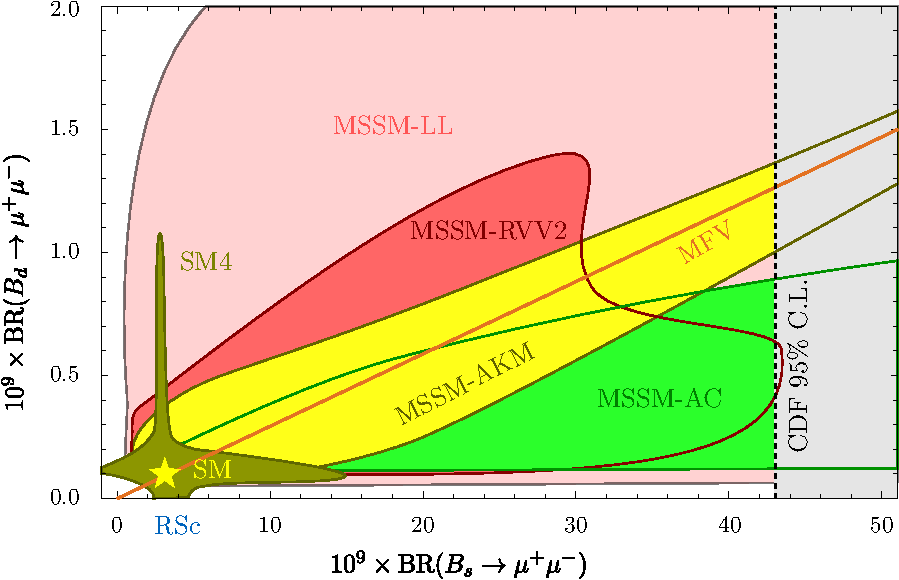
\includegraphics[width=0.8\textwidth]{./Figs/Theory/MFV.pdf}
    \caption{Correlations between the \bdmumu and \bsmumu \BFs including the SM prediction, the Minimal Flavour Violation hypothesis (MFV), four Minimal Supersymmetric Standard Models (MSSM)~\cite{Martin:1997ns} and the SM extended to constrain four generations of fermions~(SM4)~\cite{Hou:2008xd}. Figure is taken from~\cite{Straub:2010ih}.}
    \label{fig:ratio}
\end{figure}
The MFV hypothesis predicts that the coupling of quark flavour and $\mathcal{CP}$ violation follow the same Yukawa structure as the SM in NP models. It is a popular theory to describe the flavour structure in NP models due to the current agreement of measurements with the SM predictions. A significant deviation of the \BF ratio from the SM or MFV hypothesis predictions would indicate the need to a new flavour structure in theoretical models.

Additionally NP models could move the \BFs and \ADG away from the SM predictions by providing new particles that can contribute to the decays. These new particles would change the Wilson coefficients included in the parameters $P$ and $S$. The dependence of the \BFs and \ADG on $P$ and $S$ are different, as shown in Equations~\ref{eq:BF_form} and~\ref{eq:NP_ADG}, therefore NP models can influence the observables independently. The allowed values of \ADG and the ratio of the measured \BF to prompt SM prediction are shown in Figure~\ref{fig:NPmodelsB} for possible situations where $S=0$, $P=1$, $P\pm S = 1$ and $\varphi_P, \varphi_S \in {0, \pi}$. These figures illustrate that if NP effects are not revealed in the \BF measurements, they could still appear in \ADG. Furthermore in some scenarios \ADG is needed to resolve degeneracies that arise from information from the \BF alone.
\begin{figure}[tbp]
    \centering
        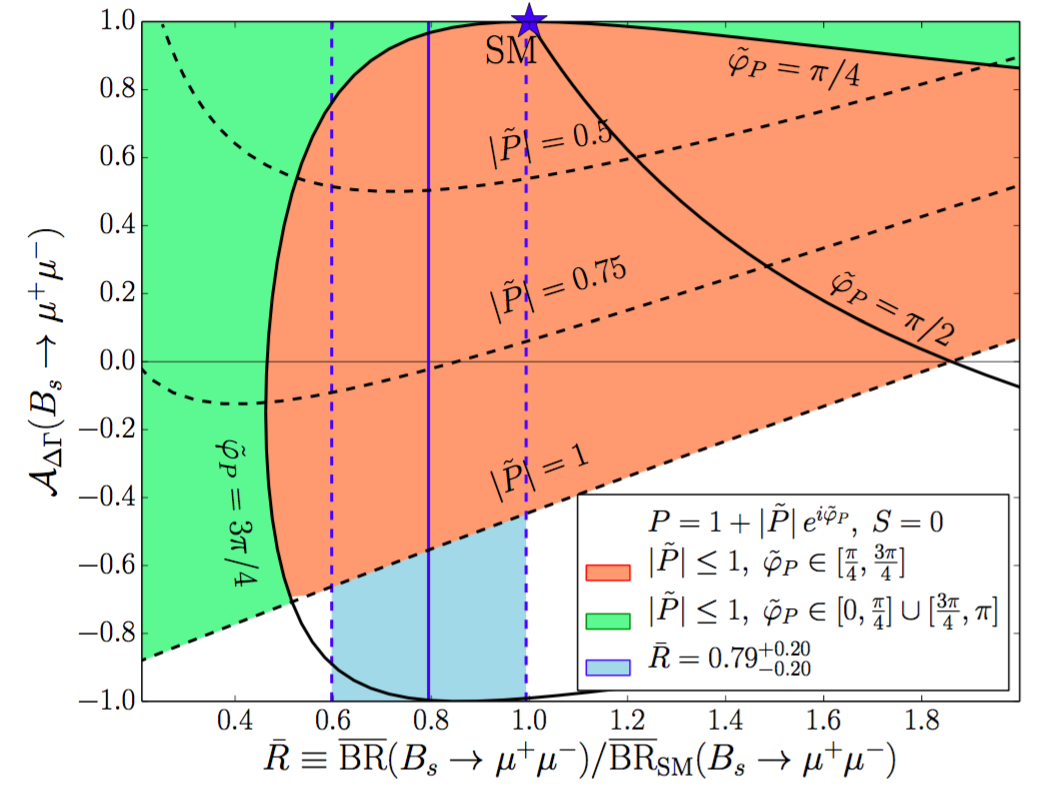
\includegraphics[width=0.49\textwidth]{./Figs/Theory/NP_S_0.png}
        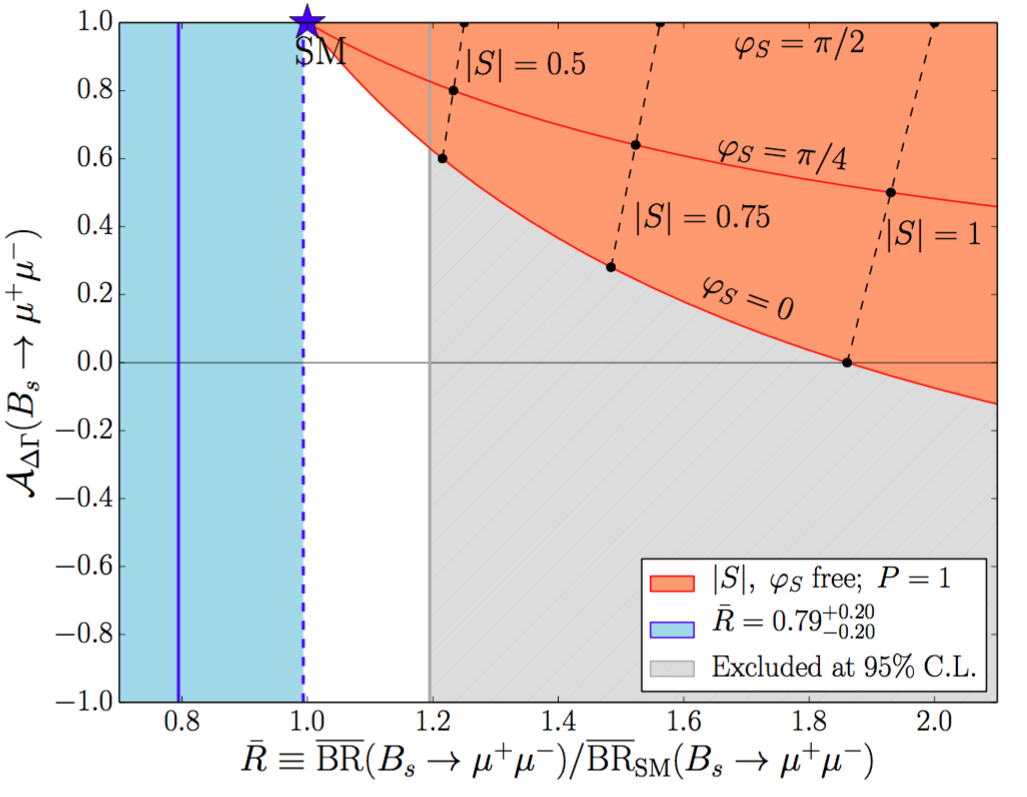
\includegraphics[width=0.49\textwidth]{./Figs/Theory/NP_P_1.png}
        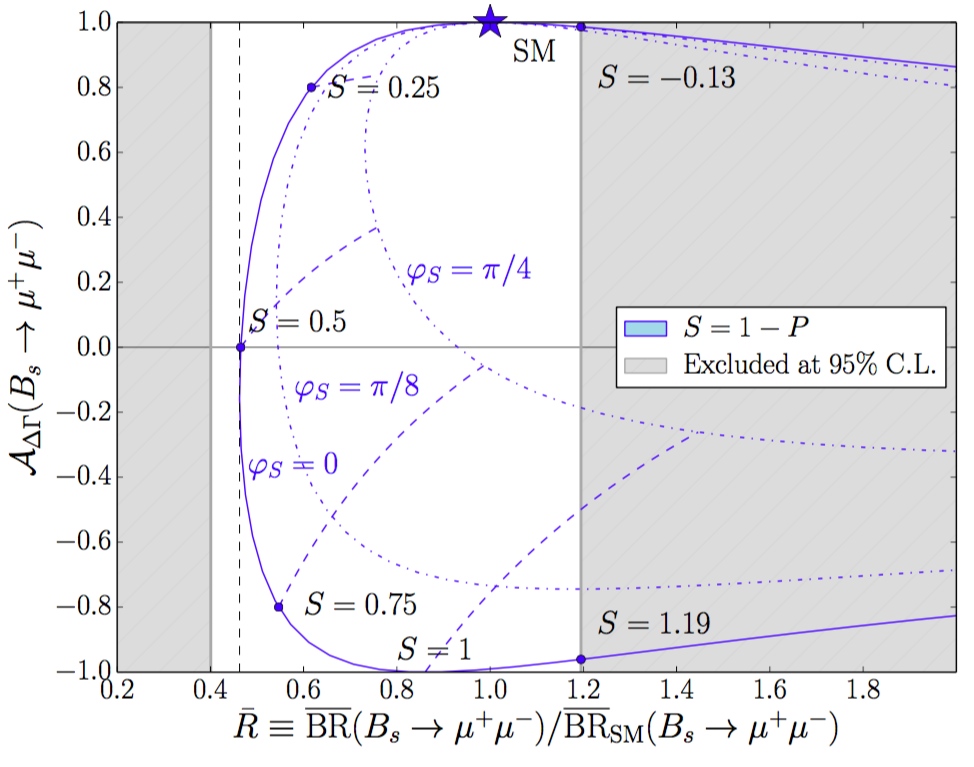
\includegraphics[width=0.49\textwidth]{./Figs/Theory/NP_P_pm_S_1.png}        
        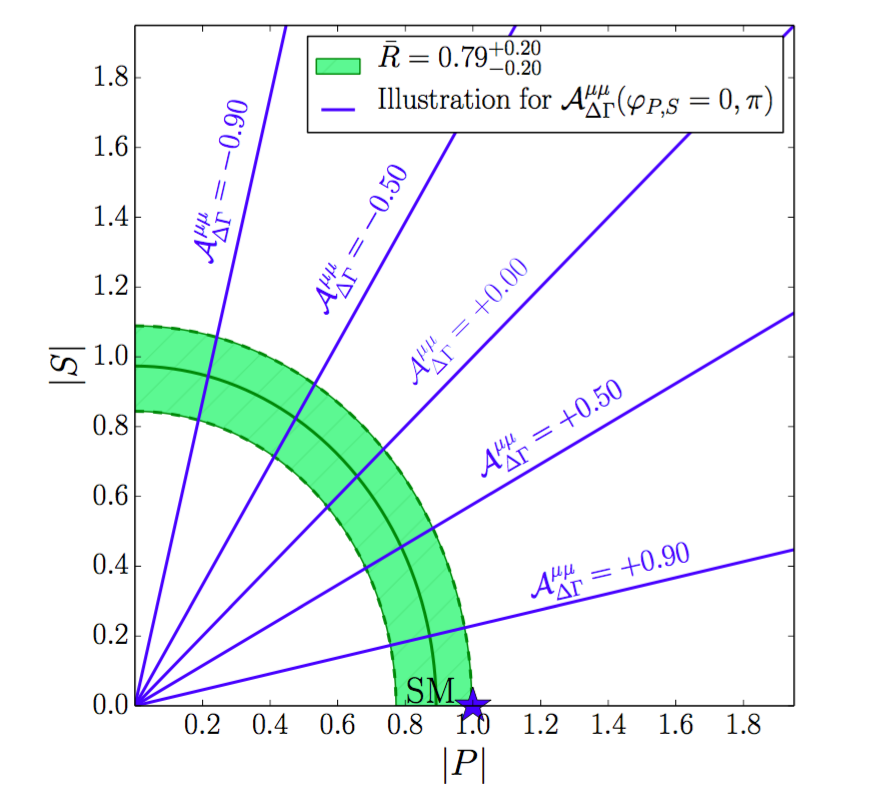
\includegraphics[width=0.45\textwidth]{./Figs/Theory/NP_phi.png}
    \caption{Allowed values for $\mathcal{B}$(\bsmumu) and \ADG for situations where $S=0$ (top left), $P=1$ (top right), $P \pm S = 1$ (bottom left) and $\varphi_P, \varphi_S \in {0, \pi}$ (bottom right)~\cite{Buras:2013uqa,Knegjens:2014zva}. The ratio $\overline{R}$ plotted is from an average of the individual results from the CMS and LHCb collaborations from~\cite{CMSandLHCbCollaborations:2013pla}, the results from the combined analysis of the CMS and LHCb data gives $\overline{R} = 0.76^{+0.2}_{-0.18}$~\cite{CMS:2014xfa}.}
    \label{fig:NPmodelsB}
\end{figure}

Amongst the BSM theories that can influence the values of $P$ and $S$ are the two Higgs doublet model (2HDM)~\cite{HALL1981397}, supersymmetric models~\cite{Witten:1981nf}, models including leptoquarks and models that obey the MFV hypothesis as mentioned earlier.

The 2HDM extends the Higgs sector of the SM by introducing two complex scalar field doublets both with non-zero vacuum expectation values. Spontaneous symmetry breaking then produces 2 charged, one neutral pseudoscalar and 2 neutral scalar Higgs bosons. The new particles can enter the loops of \bmumu decays and allow FCNCs to occur that the tree level. Different scenarios of this model depend on the Higgs-quark interactions and can incorporate the MFV hypothesis. This model can produce scenarios where $S=0$, $P=1$ or $P\pm S = 1$~\cite{Buras:2013uqa,Knegjens:2014zva} and the corresponding \BF and \ADG values for \bsmumu decays as shown in Figure~\ref{fig:NPmodelsB}.

Supersymmetric (SUSY) models extend the SM by giving each SM particle a supersymmetric partner. The resulting theory is symmetric under the transformation of fermions to boson and bosons to fermions. So far no evidence for SUSY particles has been found therefore the symmetry must be broken and the mass of SUSY particles is greater than their SM partners. The Minimal Supersymmetric Standard Model (MSSM) includes a Higgs sector similar to the 2HDM and there are scenarios where it obeys the MFV hypothesis. \bmumu decays are sensitive to this model provided the ratio of the vacuum expectations values of the Higgs doublet is large~\cite{Babu:1999hn,Isidori:2001fv,Buras:2002vd}. The MSSM can produce values for \ADG and the \bsmumu \BF shown in Figure~\ref{fig:NPmodelsB} for situations where $P\pm S =1$ and $\varphi_P, \varphi_S \in {0, \pi}$~\cite{Buras:2013uqa,Knegjens:2014zva}.

Models including leptoquarks are currently popular to explain the anomalies observed in heavy flavour measurements~\cite{Barbieri:2016las,Becirevic:2016yqi,Hiller:2014yaa,Bauer:2015knc,Fajfer:2015ycq}. A leptoquark is a boson that carries both lepton and baryons numbers. The exact quantum numbers depend on the interactions with SM fermions and leptoquarks can enable FCNCs to occur at the tree level. Therefore leptoquarks could enhance \bmumu decays but information from \ADG is necessary for the study of leptoquarks with \bmumu decays because it resolves degeneracies that are present with just the \BF measurements~\cite{Altmannshofer:2017wqy}.

Although \bmumu decays are yet to reveal NP, the current experimental precision still leaves plenty of room for NP to be revealed. The observation of \bsmumu decays makes it possible to start investigating \ADG through the \bsmumu \el. A measurement of \ADG will proved important information, complementary to the \bmumu \BF measurements to search for NP in \bsmumu decays.


%%*******************************************************************************
%*********************************** First Chapter *****************************
%*******************************************************************************

\chapter{Getting started}  %Title of the First Chapter

\ifpdf
    \graphicspath{{Chapter1/Figs/Raster/}{Chapter1/Figs/PDF/}{Chapter1/Figs/}}
\else
    \graphicspath{{Chapter1/Figs/Vector/}{Chapter1/Figs/}}
\fi


%********************************** %First Section  **************************************
\section{What is loren ipsum? Title with math \texorpdfstring{$\sigma$}{[sigma]}} %Section - 1.1 

Lorem Ipsum is simply dummy text of the printing and typesetting industry (see 
Section~\ref{section1.3}). Lorem Ipsum~\citep{Aup91} has been the industry's 
standard dummy text ever since the 1500s, when an unknown printer took a galley 
of type and scrambled it to make a type specimen book. It has survived not only 
five centuries, but also the leap into electronic typesetting, remaining 
essentially unchanged. It was popularised in the 1960s with the release of 
Letraset sheets containing Lorem Ipsum passages, and more recently with desktop 
publishing software like Aldus PageMaker including versions of Lorem 
Ipsum~\citep{AAB95,Con90,LM65}.

The most famous equation in the world: $E^2 = (m_0c^2)^2 + (pc)^2$, which is 
known as the \textbf{energy-mass-momentum} relation as an in-line equation.

A {\em \LaTeX{} class file}\index{\LaTeX{} class file@LaTeX class file} is a file, which holds style information for a particular \LaTeX{}.


\begin{align}
CIF: \hspace*{5mm}F_0^j(a) = \frac{1}{2\pi \iota} \oint_{\gamma} \frac{F_0^j(z)}{z - a} dz
\end{align}

\nomenclature[z-cif]{$CIF$}{Cauchy's Integral Formula}                                % first letter Z is for Acronyms 
\nomenclature[a-F]{$F$}{complex function}                                                   % first letter A is for Roman symbols
\nomenclature[g-p]{$\pi$}{ $\simeq 3.14\ldots$}                                             % first letter G is for Greek Symbols
\nomenclature[g-i]{$\iota$}{unit imaginary number $\sqrt{-1}$}                      % first letter G is for Greek Symbols
\nomenclature[g-g]{$\gamma$}{a simply closed curve on a complex plane}  % first letter G is for Greek Symbols
\nomenclature[x-i]{$\oint_\gamma$}{integration around a curve $\gamma$} % first letter X is for Other Symbols
\nomenclature[r-j]{$j$}{superscript index}                                                       % first letter R is for superscripts
\nomenclature[s-0]{$0$}{subscript index}                                                        % first letter S is for subscripts


%********************************** %Second Section  *************************************
\section{Why do we use loren ipsum?} %Section - 1.2


It is a long established fact that a reader will be distracted by the readable content of a page when looking at its layout. The point of using Lorem Ipsum is that it has a more-or-less normal distribution of letters, as opposed to using `Content here, content here', making it look like readable English. Many desktop publishing packages and web page editors now use Lorem Ipsum as their default model text, and a search for `lorem ipsum' will uncover many web sites still in their infancy. Various versions have evolved over the years, sometimes by accident, sometimes on purpose (injected humour and the like).

%********************************** % Third Section  *************************************
\section{Where does it come from?}  %Section - 1.3 
\label{section1.3}

Contrary to popular belief, Lorem Ipsum is not simply random text. It has roots in a piece of classical Latin literature from 45 BC, making it over 2000 years old. Richard McClintock, a Latin professor at Hampden-Sydney College in Virginia, looked up one of the more obscure Latin words, consectetur, from a Lorem Ipsum passage, and going through the cites of the word in classical literature, discovered the undoubtable source. Lorem Ipsum comes from sections 1.10.32 and 1.10.33 of "de Finibus Bonorum et Malorum" (The Extremes of Good and Evil) by Cicero, written in 45 BC. This book is a treatise on the theory of ethics, very popular during the Renaissance. The first line of Lorem Ipsum, "Lorem ipsum dolor sit amet..", comes from a line in section 1.10.32.

The standard chunk of Lorem Ipsum used since the 1500s is reproduced below for those interested. Sections 1.10.32 and 1.10.33 from ``de Finibus Bonorum et Malorum" by Cicero are also reproduced in their exact original form, accompanied by English versions from the 1914 translation by H. Rackham

``Lorem ipsum dolor sit amet, consectetur adipisicing elit, sed do eiusmod tempor incididunt ut labore et dolore magna aliqua. Ut enim ad minim veniam, quis nostrud exercitation ullamco laboris nisi ut aliquip ex ea commodo consequat. Duis aute irure dolor in reprehenderit in voluptate velit esse cillum dolore eu fugiat nulla pariatur. Excepteur sint occaecat cupidatat non proident, sunt in culpa qui officia deserunt mollit anim id est laborum."

Section 1.10.32 of ``de Finibus Bonorum et Malorum", written by Cicero in 45 BC: ``Sed ut perspiciatis unde omnis iste natus error sit voluptatem accusantium doloremque laudantium, totam rem aperiam, eaque ipsa quae ab illo inventore veritatis et quasi architecto beatae vitae dicta sunt explicabo. Nemo enim ipsam voluptatem quia voluptas sit aspernatur aut odit aut fugit, sed quia consequuntur magni dolores eos qui ratione voluptatem sequi nesciunt. Neque porro quisquam est, qui dolorem ipsum quia dolor sit amet, consectetur, adipisci velit, sed quia non numquam eius modi tempora incidunt ut labore et dolore magnam aliquam quaerat voluptatem. Ut enim ad minima veniam, quis nostrum exercitationem ullam corporis suscipit laboriosam, nisi ut aliquid ex ea commodi consequatur? Quis autem vel eum iure reprehenderit qui in ea voluptate velit esse quam nihil molestiae consequatur, vel illum qui dolorem eum fugiat quo voluptas nulla pariatur?"

1914 translation by H. Rackham: ``But I must explain to you how all this mistaken idea of denouncing pleasure and praising pain was born and I will give you a complete account of the system, and expound the actual teachings of the great explorer of the truth, the master-builder of human happiness. No one rejects, dislikes, or avoids pleasure itself, because it is pleasure, but because those who do not know how to pursue pleasure rationally encounter consequences that are extremely painful. Nor again is there anyone who loves or pursues or desires to obtain pain of itself, because it is pain, but because occasionally circumstances occur in which toil and pain can procure him some great pleasure. To take a trivial example, which of us ever undertakes laborious physical exercise, except to obtain some advantage from it? But who has any right to find fault with a man who chooses to enjoy a pleasure that has no annoying consequences, or one who avoids a pain that produces no resultant pleasure?"

Section 1.10.33 of ``de Finibus Bonorum et Malorum", written by Cicero in 45 BC: ``At vero eos et accusamus et iusto odio dignissimos ducimus qui blanditiis praesentium voluptatum deleniti atque corrupti quos dolores et quas molestias excepturi sint occaecati cupiditate non provident, similique sunt in culpa qui officia deserunt mollitia animi, id est laborum et dolorum fuga. Et harum quidem rerum facilis est et expedita distinctio. Nam libero tempore, cum soluta nobis est eligendi optio cumque nihil impedit quo minus id quod maxime placeat facere possimus, omnis voluptas assumenda est, omnis dolor repellendus. Temporibus autem quibusdam et aut officiis debitis aut rerum necessitatibus saepe eveniet ut et voluptates repudiandae sint et molestiae non recusandae. Itaque earum rerum hic tenetur a sapiente delectus, ut aut reiciendis voluptatibus maiores alias consequatur aut perferendis doloribus asperiores repellat."

1914 translation by H. Rackham: ``On the other hand, we denounce with righteous indignation and dislike men who are so beguiled and demoralized by the charms of pleasure of the moment, so blinded by desire, that they cannot foresee the pain and trouble that are bound to ensue; and equal blame belongs to those who fail in their duty through weakness of will, which is the same as saying through shrinking from toil and pain. These cases are perfectly simple and easy to distinguish. In a free hour, when our power of choice is untrammelled and when nothing prevents our being able to do what we like best, every pleasure is to be welcomed and every pain avoided. But in certain circumstances and owing to the claims of duty or the obligations of business it will frequently occur that pleasures have to be repudiated and annoyances accepted. The wise man therefore always holds in these matters to this principle of selection: he rejects pleasures to secure other greater pleasures, or else he endures pains to avoid worse pains."

\nomenclature[z-DEM]{DEM}{Discrete Element Method}
\nomenclature[z-FEM]{FEM}{Finite Element Method}
\nomenclature[z-PFEM]{PFEM}{Particle Finite Element Method}
\nomenclature[z-FVM]{FVM}{Finite Volume Method}
\nomenclature[z-BEM]{BEM}{Boundary Element Method}
\nomenclature[z-MPM]{MPM}{Material Point Method}
\nomenclature[z-LBM]{LBM}{Lattice Boltzmann Method}
\nomenclature[z-MRT]{MRT}{Multi-Relaxation 
Time}
\nomenclature[z-RVE]{RVE}{Representative Elemental Volume}
\nomenclature[z-GPU]{GPU}{Graphics Processing Unit}
\nomenclature[z-SH]{SH}{Savage Hutter}
\nomenclature[z-CFD]{CFD}{Computational Fluid Dynamics}
\nomenclature[z-LES]{LES}{Large Eddy Simulation}
\nomenclature[z-FLOP]{FLOP}{Floating Point Operations}
\nomenclature[z-ALU]{ALU}{Arithmetic Logic Unit}
\nomenclature[z-FPU]{FPU}{Floating Point Unit}
\nomenclature[z-SM]{SM}{Streaming Multiprocessors}
\nomenclature[z-PCI]{PCI}{Peripheral Component Interconnect}
\nomenclature[z-CK]{CK}{Carman - Kozeny}
\nomenclature[z-CD]{CD}{Contact Dynamics}
\nomenclature[z-DNS]{DNS}{Direct Numerical Simulation}
\nomenclature[z-EFG]{EFG}{Element-Free Galerkin}
\nomenclature[z-PIC]{PIC}{Particle-in-cell}
\nomenclature[z-USF]{USF}{Update Stress First}
\nomenclature[z-USL]{USL}{Update Stress Last}
\nomenclature[s-crit]{crit}{Critical state}
\nomenclature[z-DKT]{DKT}{Draft Kiss Tumble}
\nomenclature[z-PPC]{PPC}{Particles per cell}
%%*******************************************************************************
%****************************** Second Chapter *********************************
%*******************************************************************************

\chapter{My second chapter}

\ifpdf
    \graphicspath{{Chapter2/Figs/Raster/}{Chapter2/Figs/PDF/}{Chapter2/Figs/}}
\else
    \graphicspath{{Chapter2/Figs/Vector/}{Chapter2/Figs/}}
\fi


\section[Short title]{Reasonably long section title}

% Uncomment this line, when you have siunitx package loaded.
%The SI Units for dynamic viscosity is \si{\newton\second\per\metre\squared}.
I'm going to randomly include a picture Figure~\ref{fig:minion}.


If you have trouble viewing this document contact Krishna at: \href{mailto:kks32@cam.ac.uk}{kks32@cam.ac.uk} or raise an issue at \url{https://github.com/kks32/phd-thesis-template/}


\begin{figure}[htbp!] 
\centering    

\includegraphics[width=1.0\textwidth]{minion}
\caption[Minion]{This is just a long figure caption for the minion in Despicable Me from Pixar}
\label{fig:minion}
\end{figure}


\section*{Enumeration}
Lorem ipsum dolor sit amet, consectetur adipiscing elit. Sed vitae laoreet lectus. Donec lacus quam, malesuada ut erat vel, consectetur eleifend tellus. Aliquam non feugiat lacus. Interdum et malesuada fames ac ante ipsum primis in faucibus. Quisque a dolor sit amet dui malesuada malesuada id ac metus. Phasellus posuere egestas mauris, sed porta arcu vulputate ut. Donec arcu erat, ultrices et nisl ut, ultricies facilisis urna. Quisque iaculis, lorem non maximus pretium, dui eros auctor quam, sed sodales libero felis vel orci. Aliquam neque nunc, elementum id accumsan eu, varius eu enim. Aliquam blandit ante et ligula tempor pharetra. Donec molestie porttitor commodo. Integer rutrum turpis ac erat tristique cursus. Sed venenatis urna vel tempus venenatis. Nam eu rhoncus eros, et condimentum elit. Quisque risus turpis, aliquam eget euismod id, gravida in odio. Nunc elementum nibh risus, ut faucibus mauris molestie eu.
 Vivamus quis nunc nec nisl vulputate fringilla. Duis tempus libero ac justo laoreet tincidunt. Fusce sagittis gravida magna, pharetra venenatis mauris semper at. Nullam eleifend felis a elementum sagittis. In vel turpis eu metus euismod tempus eget sit amet tortor. Donec eu rhoncus libero, quis iaculis lectus. Aliquam erat volutpat. Proin id ullamcorper tortor. Fusce vestibulum a enim non volutpat. Nam ut interdum nulla. Proin lacinia felis malesuada arcu aliquet fringilla. Aliquam condimentum, tellus eget maximus porttitor, quam sem luctus massa, eu fermentum arcu diam ac massa. Praesent ut quam id leo molestie rhoncus. Praesent nec odio eget turpis bibendum eleifend non sit amet mi. Curabitur placerat finibus velit, eu ultricies risus imperdiet ut. Suspendisse lorem orci, luctus porta eros a, commodo maximus nisi.

Nunc et dolor diam. Phasellus eu justo vitae diam vehicula tristique. Vestibulum vulputate cursus turpis nec commodo. Etiam elementum sit amet erat et pellentesque. In eu augue sed tortor mollis tincidunt. Mauris eros dui, sagittis vestibulum vestibulum vitae, molestie a velit. Donec non felis ut velit aliquam convallis sit amet sit amet velit. Aliquam vulputate, elit in lacinia lacinia, odio lacus consectetur quam, sit amet facilisis mi justo id magna. Curabitur aliquet pulvinar eros. Cras metus enim, tristique ut magna a, interdum egestas nibh. Aenean lorem odio, varius a sollicitudin non, cursus a odio. Vestibulum ante ipsum primis in faucibus orci luctus et ultrices posuere cubilia Curae; 
\begin{enumerate}
\item The first topic is dull
\item The second topic is duller
\begin{enumerate}
\item The first subtopic is silly
\item The second subtopic is stupid
\end{enumerate}
\item The third topic is the dullest
\end{enumerate}
Morbi bibendum est aliquam, hendrerit dolor ac, pretium sem. Nunc molestie, dui in euismod finibus, nunc enim viverra enim, eu mattis mi metus id libero. Cras sed accumsan justo, ut volutpat ipsum. Nam faucibus auctor molestie. Morbi sit amet eros a justo pretium aliquet. Maecenas tempor risus sit amet tincidunt tincidunt. Curabitur dapibus gravida gravida. Vivamus porta ullamcorper nisi eu molestie. Ut pretium nisl eu facilisis tempor. Nulla rutrum tincidunt justo, id placerat lacus laoreet et. Sed cursus lobortis vehicula. Donec sed tortor et est cursus pellentesque sit amet sed velit. Proin efficitur posuere felis, porta auctor nunc. Etiam non porta risus. Pellentesque lacinia eros at ante iaculis, sed aliquet ipsum volutpat. Suspendisse potenti.

Ut ultrices lectus sed sagittis varius. Nulla facilisi. Nullam tortor sem, placerat nec condimentum eu, tristique eget ex. Nullam pretium tellus ut nibh accumsan elementum. Aliquam posuere gravida tellus, id imperdiet nulla rutrum imperdiet. Nulla pretium ullamcorper quam, non iaculis orci consectetur eget. Curabitur non laoreet nisl. Maecenas lacinia, lorem vel tincidunt cursus, odio lorem aliquet est, gravida auctor arcu urna id enim. Morbi accumsan bibendum ipsum, ut maximus dui placerat vitae. Nullam pretium ac tortor nec venenatis. Nunc non aliquet neque. 

\section*{Itemize}
\begin{itemize}
\item The first topic is dull
\item The second topic is duller
\begin{itemize}
\item The first subtopic is silly
\item The second subtopic is stupid
\end{itemize}
\item The third topic is the dullest
\end{itemize}

\section*{Description}
\begin{description}
\item[The first topic] is dull
\item[The second topic] is duller
\begin{description}
\item[The first subtopic] is silly
\item[The second subtopic] is stupid
\end{description}
\item[The third topic] is the dullest
\end{description}


\clearpage

\tochide\section{Hidden section}
\textbf{Lorem ipsum dolor sit amet}, \textit{consectetur adipiscing elit}. In magna nisi, aliquam id blandit id, congue ac est. Fusce porta consequat leo. Proin feugiat at felis vel consectetur. Ut tempus ipsum sit amet congue posuere. Nulla varius rutrum quam. Donec sed purus luctus, faucibus velit id, ultrices sapien. Cras diam purus, tincidunt eget tristique ut, egestas quis nulla. Curabitur vel iaculis lectus. Nunc nulla urna, ultrices et eleifend in, accumsan ut erat. In ut ante leo. Aenean a lacinia nisl, sit amet ullamcorper dolor. Maecenas blandit, tortor ut scelerisque congue, velit diam volutpat metus, sed vestibulum eros justo ut nulla. Etiam nec ipsum non enim luctus porta in in massa. Cras arcu urna, malesuada ut tellus ut, pellentesque mollis risus.Morbi vel tortor imperdiet arcu auctor mattis sit amet eu nisi. Nulla gravida urna vel nisl egestas varius. Aliquam posuere ante quis malesuada dignissim. Mauris ultrices tristique eros, a dignissim nisl iaculis nec. Praesent dapibus tincidunt mauris nec tempor. Curabitur et consequat nisi. Quisque viverra egestas risus, ut sodales enim blandit at. Mauris quis odio nulla. Cras euismod turpis magna, in facilisis diam congue non. Mauris faucibus nisl a orci dictum, et tempus mi cursus.

Etiam elementum tristique lacus, sit amet eleifend nibh eleifend sed \footnote{My footnote goes blah blah blah! \dots}. Maecenas dapibu augue ut urna malesuada, non tempor nibh mollis. Donec sed sem sollicitudin, convallis velit aliquam, tincidunt diam. In eu venenatis lorem. Aliquam non augue porttitor tellus faucibus porta et nec ante. Proin sodales, libero vitae commodo sodales, dolor nisi cursus magna, non tincidunt ipsum nibh eget purus. Nam rutrum tincidunt arcu, tincidunt vulputate mi sagittis id. Proin et nisi nec orci tincidunt auctor et porta elit. Praesent eu dolor ac magna cursus euismod. Integer non dictum nunc.


\begin{landscape}

\section*{Subplots}
I can cite Wall-E (see Fig.~\ref{fig:WallE}) and Minions in despicable me (Fig.~\ref{fig:Minnion}) or I can cite the whole figure as Fig.~\ref{fig:animations}


\begin{figure}
  \centering
  \begin{subfigure}[b]{0.3\textwidth}
    
\includegraphics[width=\textwidth]{TomandJerry}
    \caption{Tom and Jerry}
    \label{fig:TomJerry}   
  \end{subfigure}             
  \begin{subfigure}[b]{0.3\textwidth}
    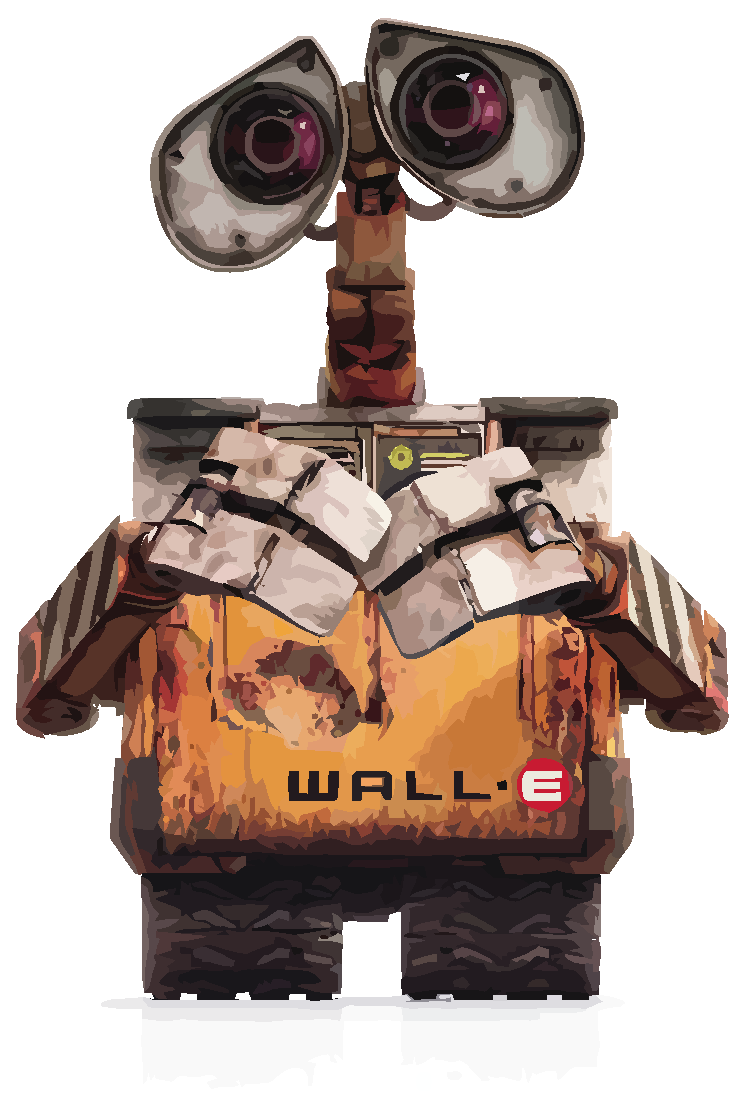
\includegraphics[width=\textwidth]{WallE}
    \caption{Wall-E}
    \label{fig:WallE}
  \end{subfigure}             
  \begin{subfigure}[b]{0.3\textwidth}
    
\includegraphics[width=\textwidth]{minion}
    \caption{Minions}
    \label{fig:Minnion}
  \end{subfigure}
  \caption{Best Animations}
  \label{fig:animations}
\end{figure}


\end{landscape}

%\chapter{My third chapter}

% **************************** Define Graphics Path **************************
\ifpdf
    \graphicspath{{Chapter3/Figs/Raster/}{Chapter3/Figs/PDF/}{Chapter3/Figs/}}
\else
    \graphicspath{{Chapter3/Figs/Vector/}{Chapter3/Figs/}}
\fi

\section{First section of the third chapter}
And now I begin my third chapter here \dots

And now to cite some more people~\citet{Rea85,Ancey1996}

\subsection{First subsection in the first section}
\dots and some more 

\subsection{Second subsection in the first section}
\dots and some more \dots

\subsubsection{First subsub section in the second subsection}
\dots and some more in the first subsub section otherwise it all looks the same
doesn't it? well we can add some text to it \dots

\subsection{Third subsection in the first section}
\dots and some more \dots

\subsubsection{First subsub section in the third subsection}
\dots and some more in the first subsub section otherwise it all looks the same
doesn't it? well we can add some text to it and some more and some more and
some more and some more and some more and some more and some more \dots

\subsubsection{Second subsub section in the third subsection}
\dots and some more in the first subsub section otherwise it all looks the same
doesn't it? well we can add some text to it \dots

\section{Second section of the third chapter}
and here I write more \dots

\section{The layout of formal tables}
This section has been modified from ``Publication quality tables in \LaTeX*''
 by Simon Fear.

The layout of a table has been established over centuries of experience and 
should only be altered in extraordinary circumstances. 

When formatting a table, remember two simple guidelines at all times:

\begin{enumerate}
  \item Never, ever use vertical rules (lines).
  \item Never use double rules.
\end{enumerate}

These guidelines may seem extreme but I have
never found a good argument in favour of breaking them. For
example, if you feel that the information in the left half of
a table is so different from that on the right that it needs
to be separated by a vertical line, then you should use two
tables instead. Not everyone follows the second guideline:

There are three further guidelines worth mentioning here as they
are generally not known outside the circle of professional
typesetters and subeditors:

\begin{enumerate}\setcounter{enumi}{2}
  \item Put the units in the column heading (not in the body of
          the table).
  \item Always precede a decimal point by a digit; thus 0.1
      {\em not} just .1.
  \item Do not use `ditto' signs or any other such convention to
      repeat a previous value. In many circumstances a blank
      will serve just as well. If it won't, then repeat the value.
\end{enumerate}

A frequently seen mistake is to use `\textbackslash begin\{center\}' \dots `\textbackslash end\{center\}' inside a figure or table environment. This center environment can cause additional vertical space. If you want to avoid that just use `\textbackslash centering'


\begin{table}
\caption{A badly formatted table}
\centering
\label{table:bad_table}
\begin{tabular}{|l|c|c|c|c|}
\hline 
& \multicolumn{2}{c}{Species I} & \multicolumn{2}{c|}{Species II} \\ 
\hline
Dental measurement  & mean & SD  & mean & SD  \\ \hline 
\hline
I1MD & 6.23 & 0.91 & 5.2  & 0.7  \\
\hline 
I1LL & 7.48 & 0.56 & 8.7  & 0.71 \\
\hline 
I2MD & 3.99 & 0.63 & 4.22 & 0.54 \\
\hline 
I2LL & 6.81 & 0.02 & 6.66 & 0.01 \\
\hline 
CMD & 13.47 & 0.09 & 10.55 & 0.05 \\
\hline 
CBL & 11.88 & 0.05 & 13.11 & 0.04\\ 
\hline 
\end{tabular}
\end{table}

\begin{table}
\caption{A nice looking table}
\centering
\label{table:nice_table}
\begin{tabular}{l c c c c}
\hline 
\multirow{2}{*}{Dental measurement} & \multicolumn{2}{c}{Species I} & \multicolumn{2}{c}{Species II} \\ 
\cline{2-5}
  & mean & SD  & mean & SD  \\ 
\hline
I1MD & 6.23 & 0.91 & 5.2  & 0.7  \\

I1LL & 7.48 & 0.56 & 8.7  & 0.71 \\

I2MD & 3.99 & 0.63 & 4.22 & 0.54 \\

I2LL & 6.81 & 0.02 & 6.66 & 0.01 \\

CMD & 13.47 & 0.09 & 10.55 & 0.05 \\

CBL & 11.88 & 0.05 & 13.11 & 0.04\\ 
\hline 
\end{tabular}
\end{table}


\begin{table}
\caption{Even better looking table using booktabs}
\centering
\label{table:good_table}
\begin{tabular}{l c c c c}
\toprule
\multirow{2}{*}{Dental measurement} & \multicolumn{2}{c}{Species I} & \multicolumn{2}{c}{Species II} \\ 
\cmidrule{2-5}
  & mean & SD  & mean & SD  \\ 
\midrule
I1MD & 6.23 & 0.91 & 5.2  & 0.7  \\

I1LL & 7.48 & 0.56 & 8.7  & 0.71 \\

I2MD & 3.99 & 0.63 & 4.22 & 0.54 \\

I2LL & 6.81 & 0.02 & 6.66 & 0.01 \\

CMD & 13.47 & 0.09 & 10.55 & 0.05 \\

CBL & 11.88 & 0.05 & 13.11 & 0.04\\ 
\bottomrule
\end{tabular}
\end{table}

%\include{Chapter4/chapter4}
%\include{Chapter5/chapter5}
%\include{Chapter6/chapter6}
%\include{Chapter7/chapter7}



% ********************************** Back Matter *******************************
% Backmatter should be commented out, if you are using appendices after References
%\backmatter

% ********************************** Bibliography ******************************
\begin{spacing}{0.9}

% To use the conventional natbib style referencing
% Bibliography style previews: http://nodonn.tipido.net/bibstyle.php
% Reference styles: http://sites.stat.psu.edu/~surajit/present/bib.htm

\bibliographystyle{apalike}
%\bibliographystyle{unsrt} % Use for unsorted references  
%\bibliographystyle{plainnat} % use this to have URLs listed in References
\cleardoublepage
\bibliography{References/references} % Path to your References.bib file


% If you would like to use BibLaTeX for your references, pass `custombib' as
% an option in the document class. The location of 'reference.bib' should be
% specified in the preamble.tex file in the custombib section.
% Comment out the lines related to natbib above and uncomment the following line.

%\printbibliography[heading=bibintoc, title={References}]


\end{spacing}

% ********************************** Appendices ********************************

\begin{appendices} % Using appendices environment for more functunality

%\chapter{{\bf Distributions of input variables for the global BDT}}
\label{sec:appendix1}
Comparison of the signal and background distributions of input variables used in the global BDT for 2011, 2012, 2015 and 2016 data taking conditions. Signal distributions are from simulated \bsmumu decays for each year that have passed the selection cuts in Table~\ref{tab:BDTpresel}. The background distributions are from \bbbarmumux decays in 2011, 2012, 2015 and 2016 data with $m_{\mu \mu} > 5447$ \mevcc and passing the selection cuts in Table~\ref{tab:BDTpresel}.
The input variables used for the global BDT are:
\begin{itemize}
\item long track isolation criteria;
\item VELO track isolation criteria;
\item $\sqrt{\Delta \phi^{2} + \Delta \eta^{2}}$, where $\Delta \phi$ is the difference in azimuthal angles of the muons and $\Delta \eta$ the difference in the pseudo-rapidity of the muons;
\item the smallest \chiIP with respect to the primary vertex of the \bsmumu of the muons;
\item \chivtx of the \bs;
\item \chiIP of the \bs with respect to the primary vertex; and
\item the angle, $\theta$, between the momentum vector of the \bs and the vector connecting the production and decay vertices of the \bs.
\end{itemize}

\begin{figure}
    \centering
    \begin{subfigure}[b]{0.48\textwidth}
        \includegraphics[trim={12cm 0 0 0},clip, width=\textwidth]{./Figs/Appendix1/signal_DeltaR.pdf}
%        \caption{ }
%        \label{fig:BDTsig}
    \end{subfigure}
    ~ %add desired spacing between images, e. g. ~, \quad, \qquad, \hfill etc. 
      %(or a blank line to force the subfigure onto a new line)
    \begin{subfigure}[b]{0.48\textwidth}
       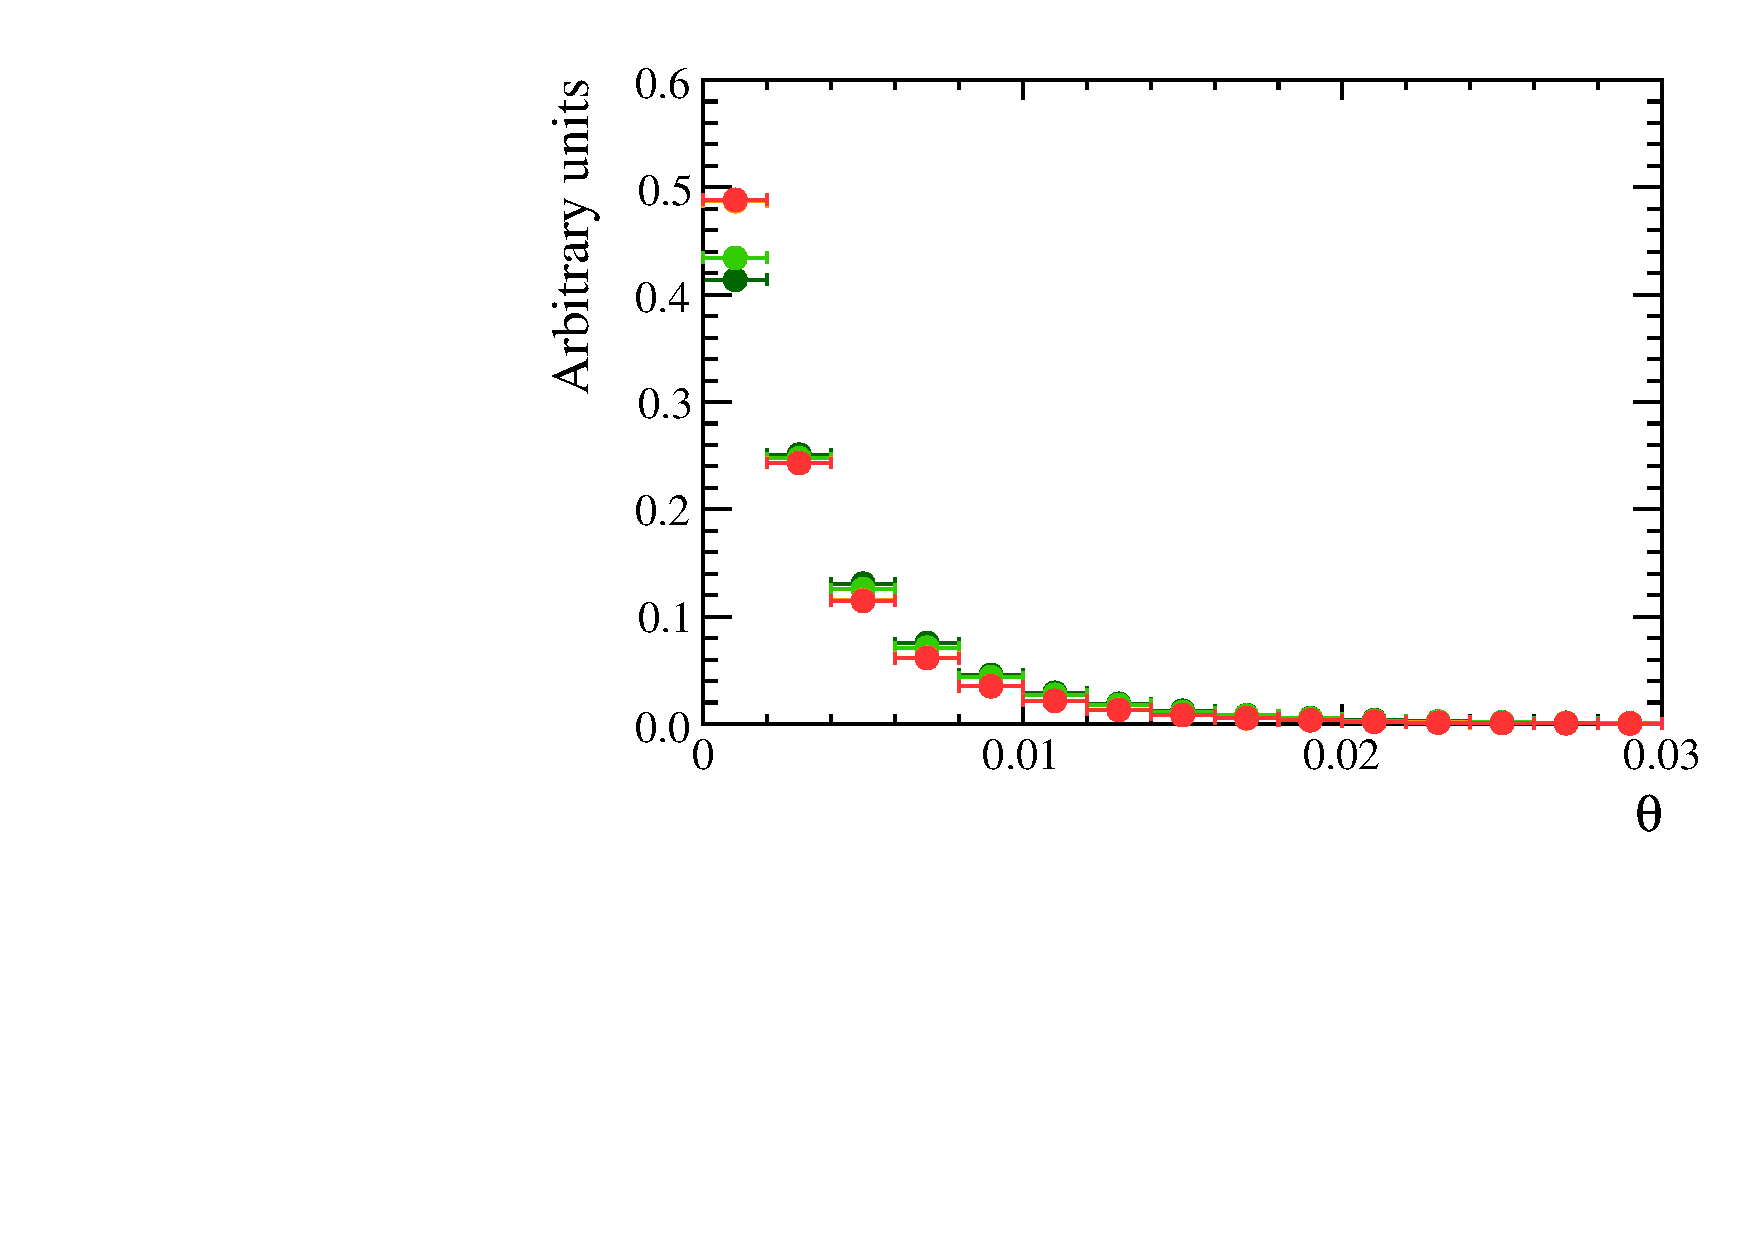
\includegraphics[width=\textwidth]{./Figs/Appendix1/signal_DIRA.pdf}
%        \caption{ }
%        \label{fig:BDTbkg}
    \end{subfigure}



 \begin{subfigure}[b]{0.48\textwidth}
        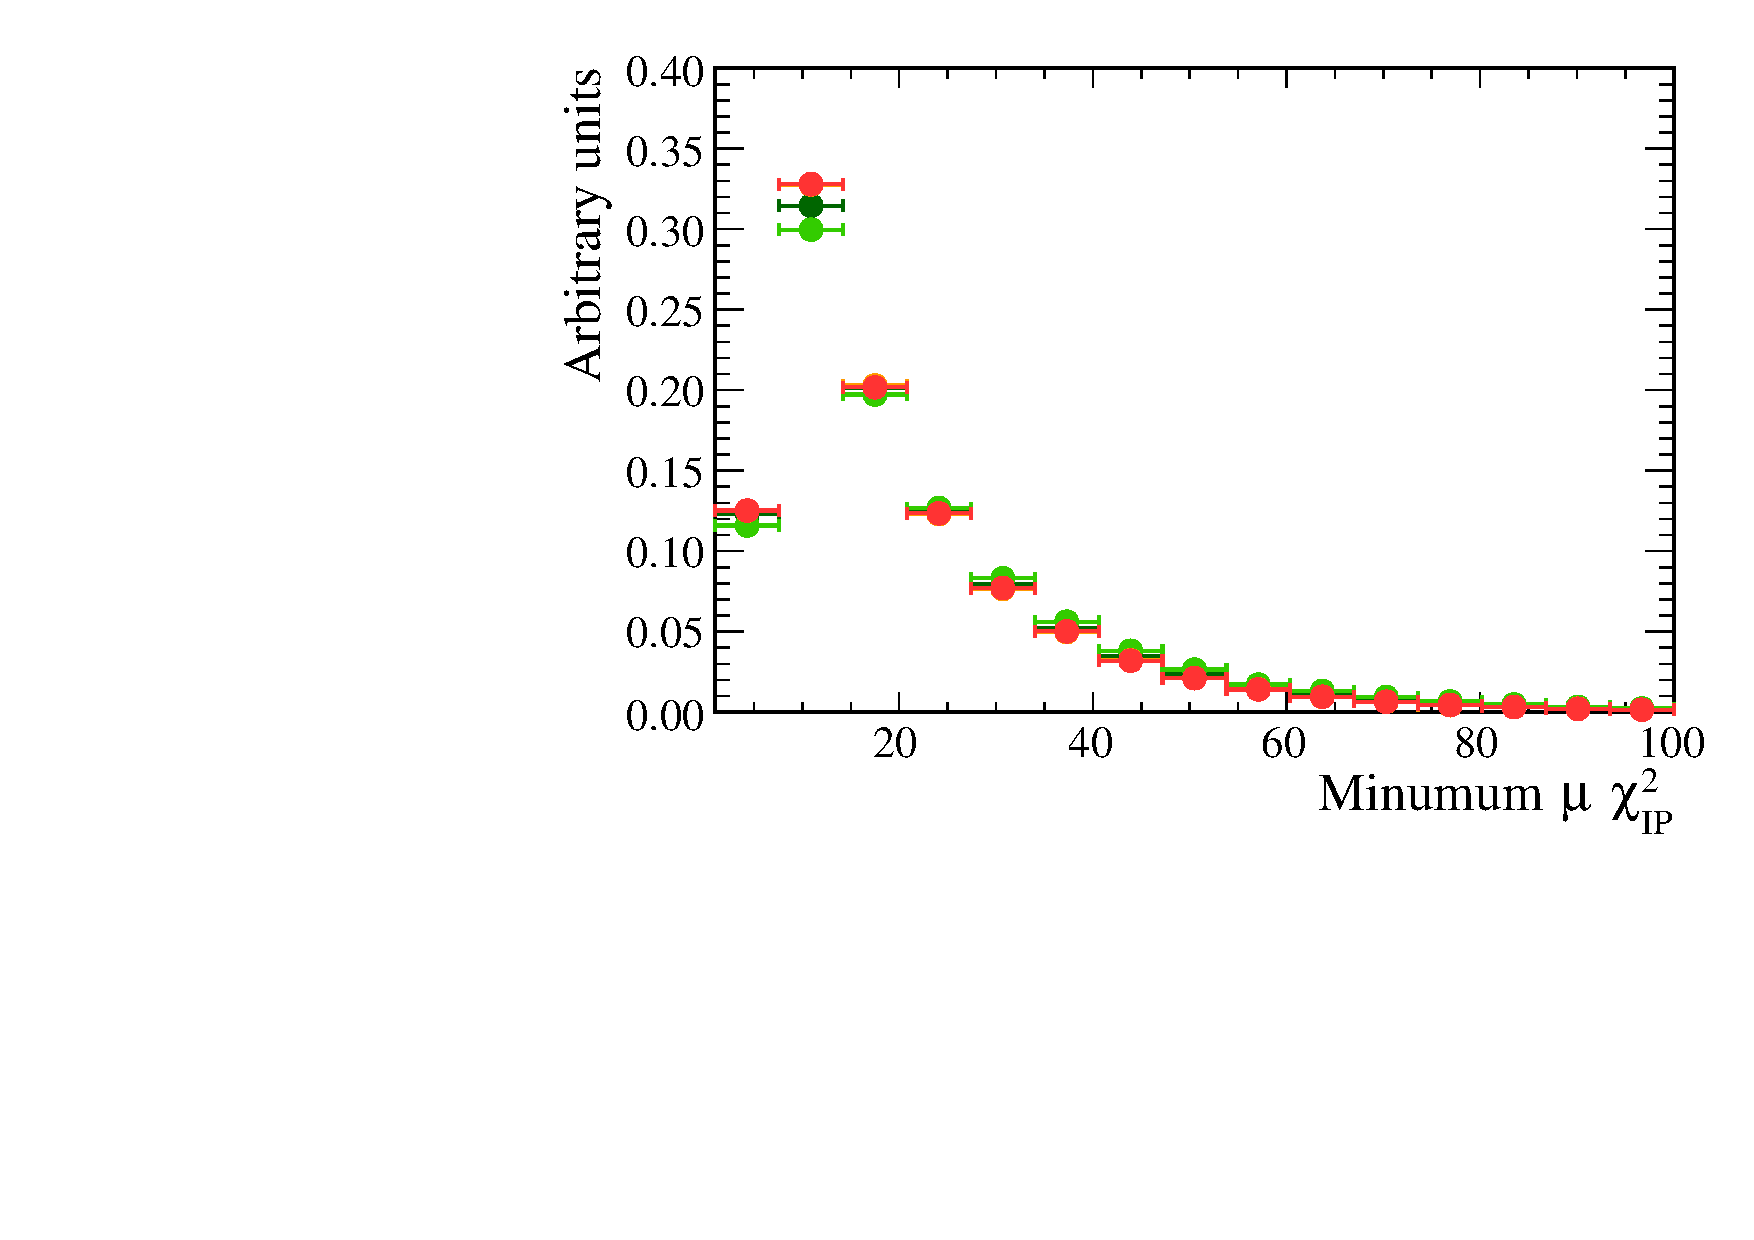
\includegraphics[width=\textwidth]{./Figs/Appendix1/signal_muIPS.pdf}
%        \caption{ }
%        \label{fig:BDTsig}
    \end{subfigure}
    ~ %add desired spacing between images, e. g. ~, \quad, \qquad, \hfill etc. 
      %(or a blank line to force the subfigure onto a new line)
    \begin{subfigure}[b]{0.48\textwidth}
       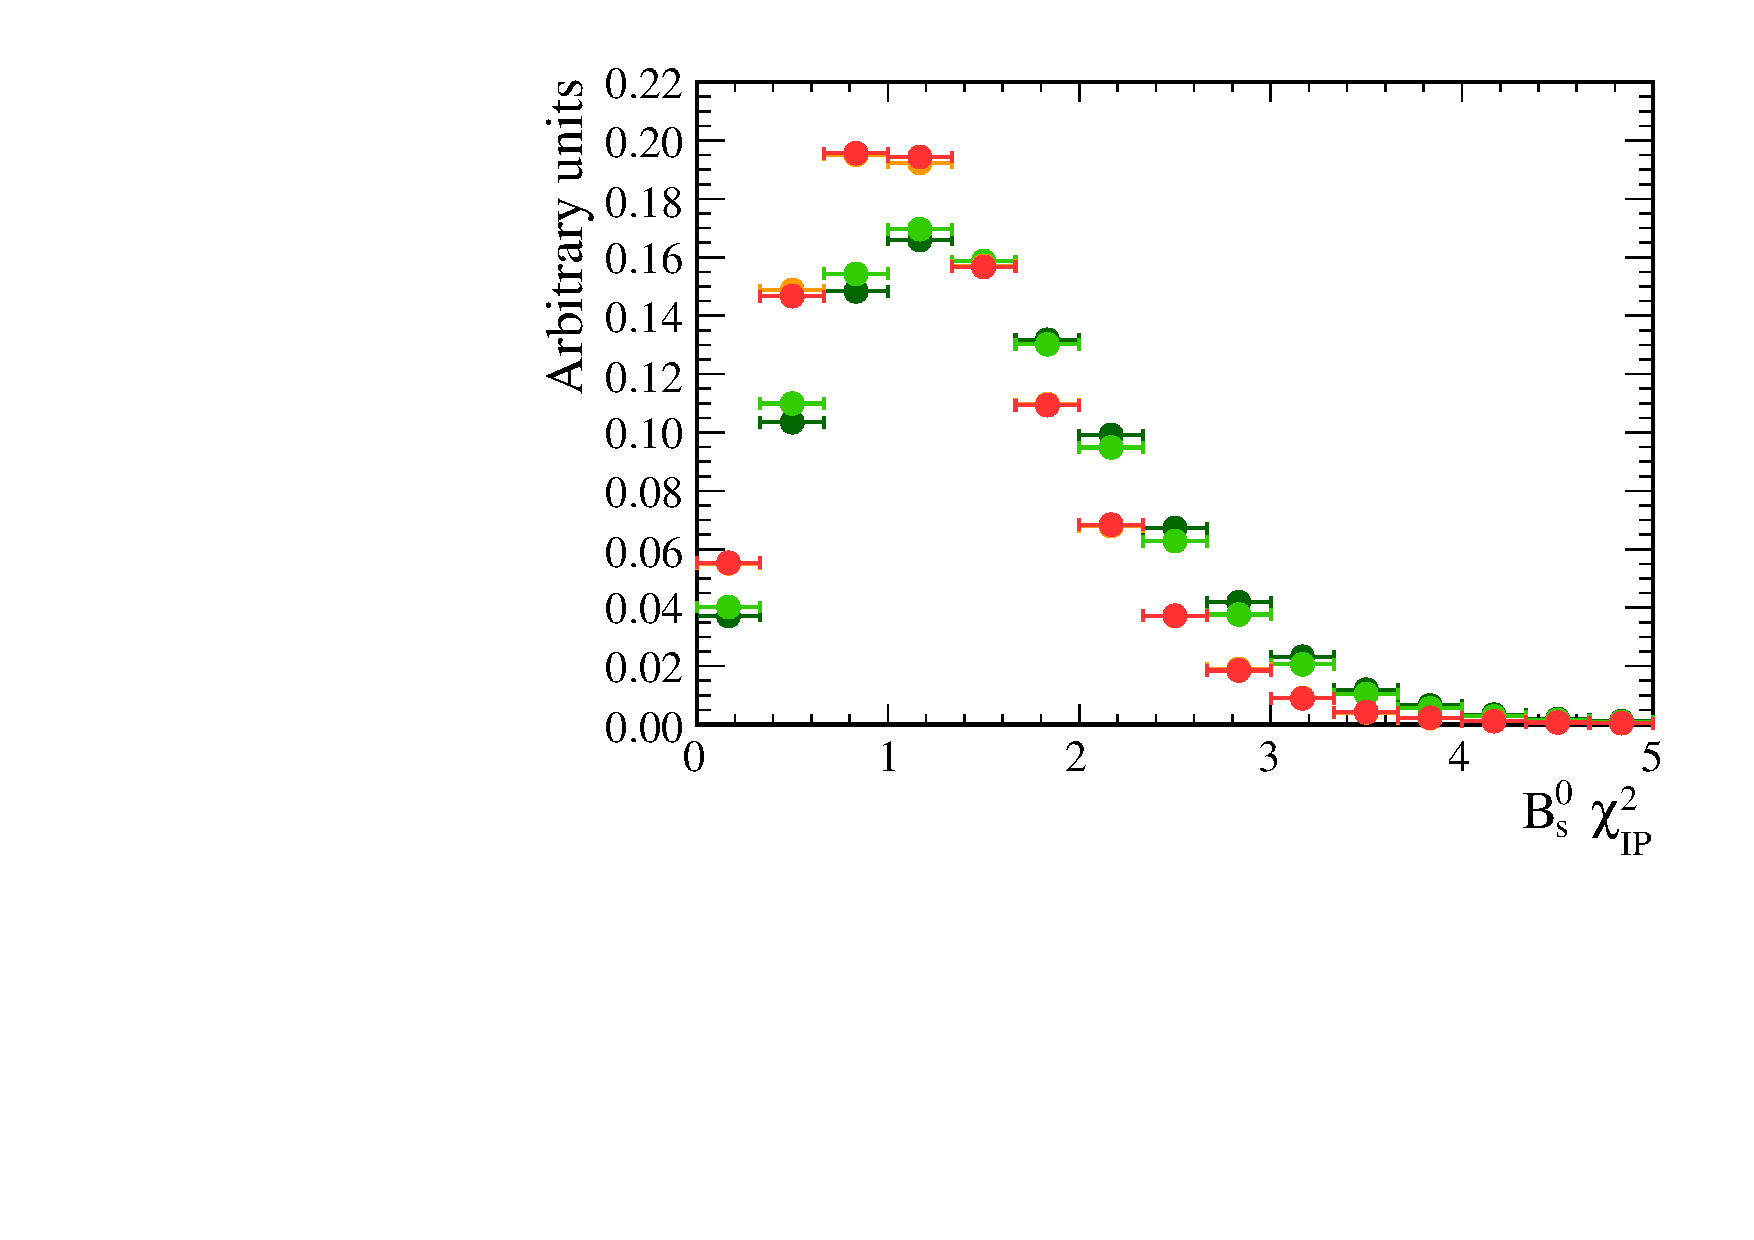
\includegraphics[width=\textwidth]{./Figs/Appendix1/signal_IPS.pdf}
%        \caption{ }
%        \label{fig:BDTbkg}
    \end{subfigure}





 \begin{subfigure}[b]{0.48\textwidth}
        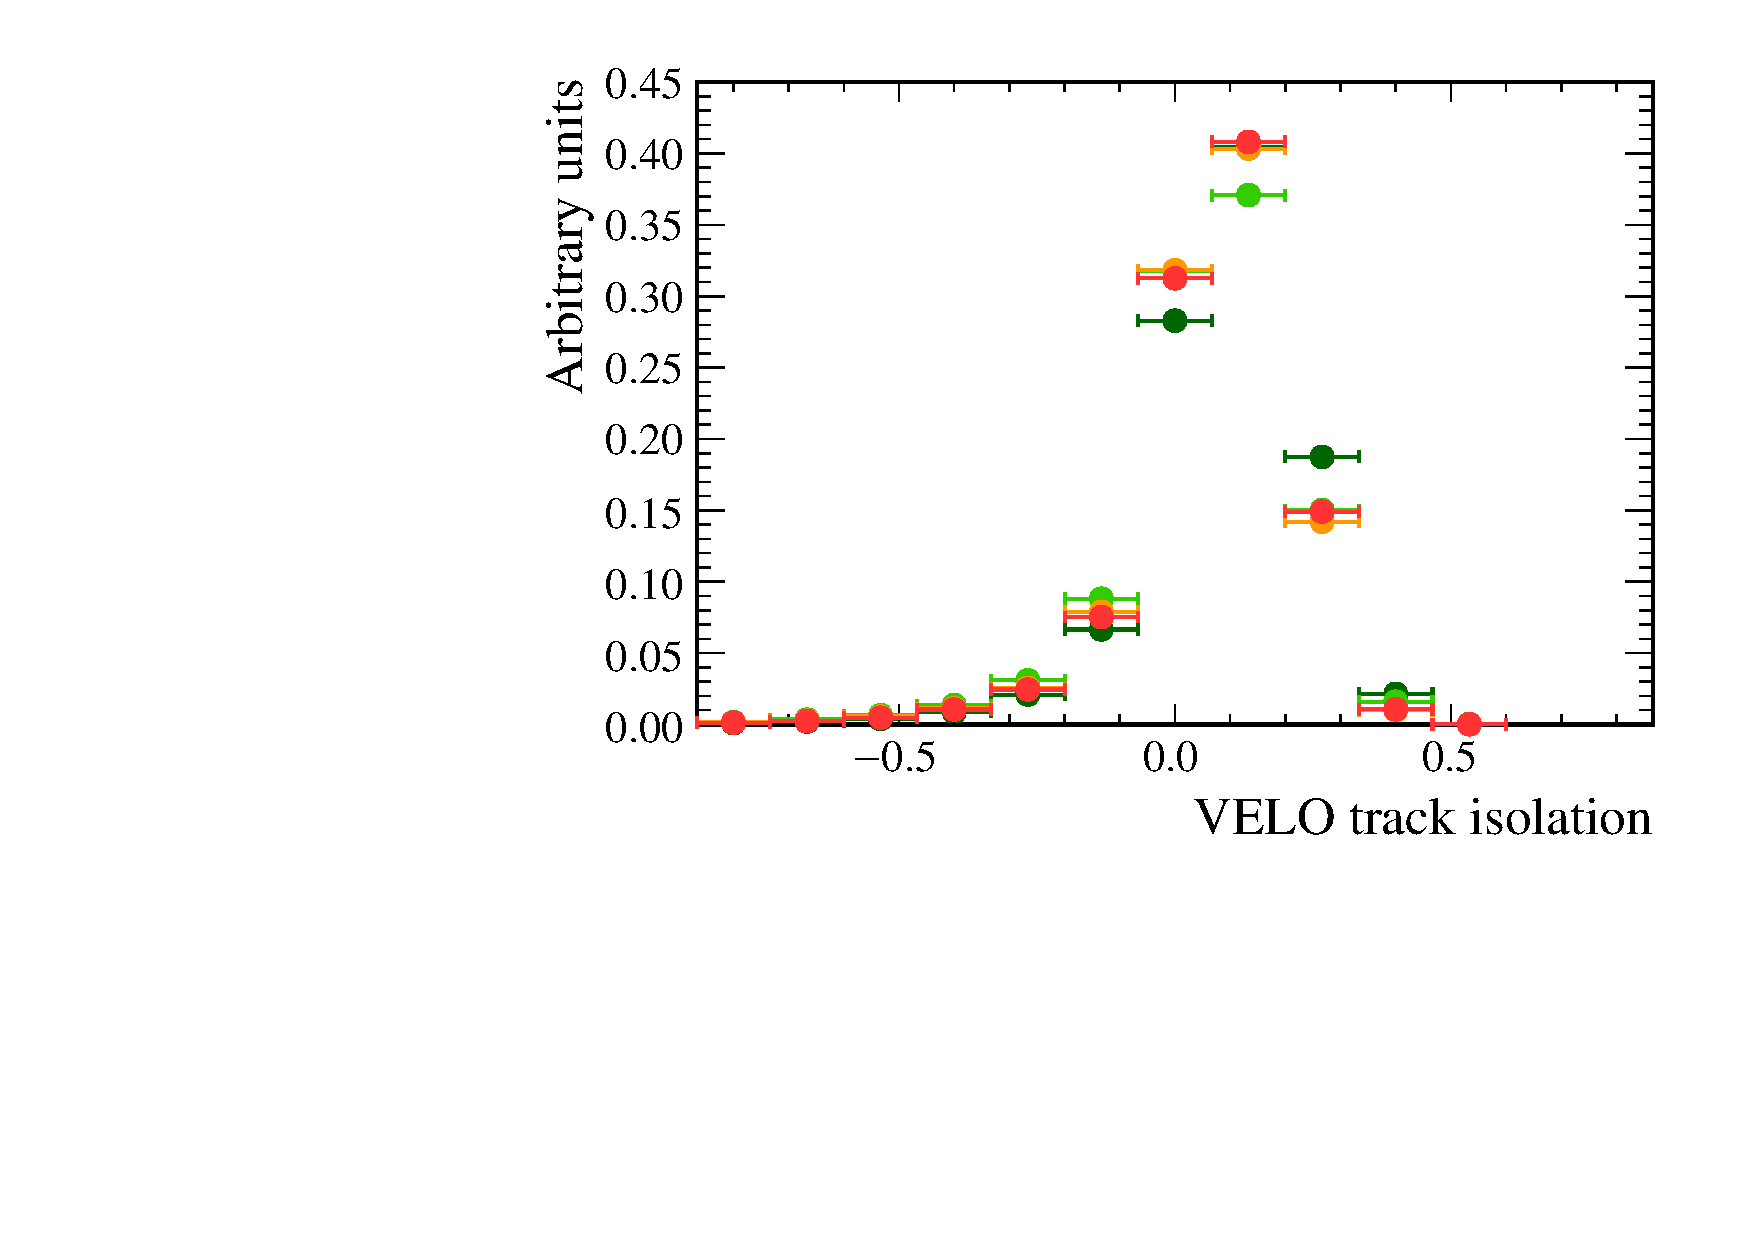
\includegraphics[width=\textwidth]{./Figs/Appendix1/signal_iso_velo.pdf}
 %       \caption{ }
 %       \label{fig:BDTsig}
    \end{subfigure}
    ~ %add desired spacing between images, e. g. ~, \quad, \qquad, \hfill etc. 
      %(or a blank line to force the subfigure onto a new line)
    \begin{subfigure}[b]{0.48\textwidth}
       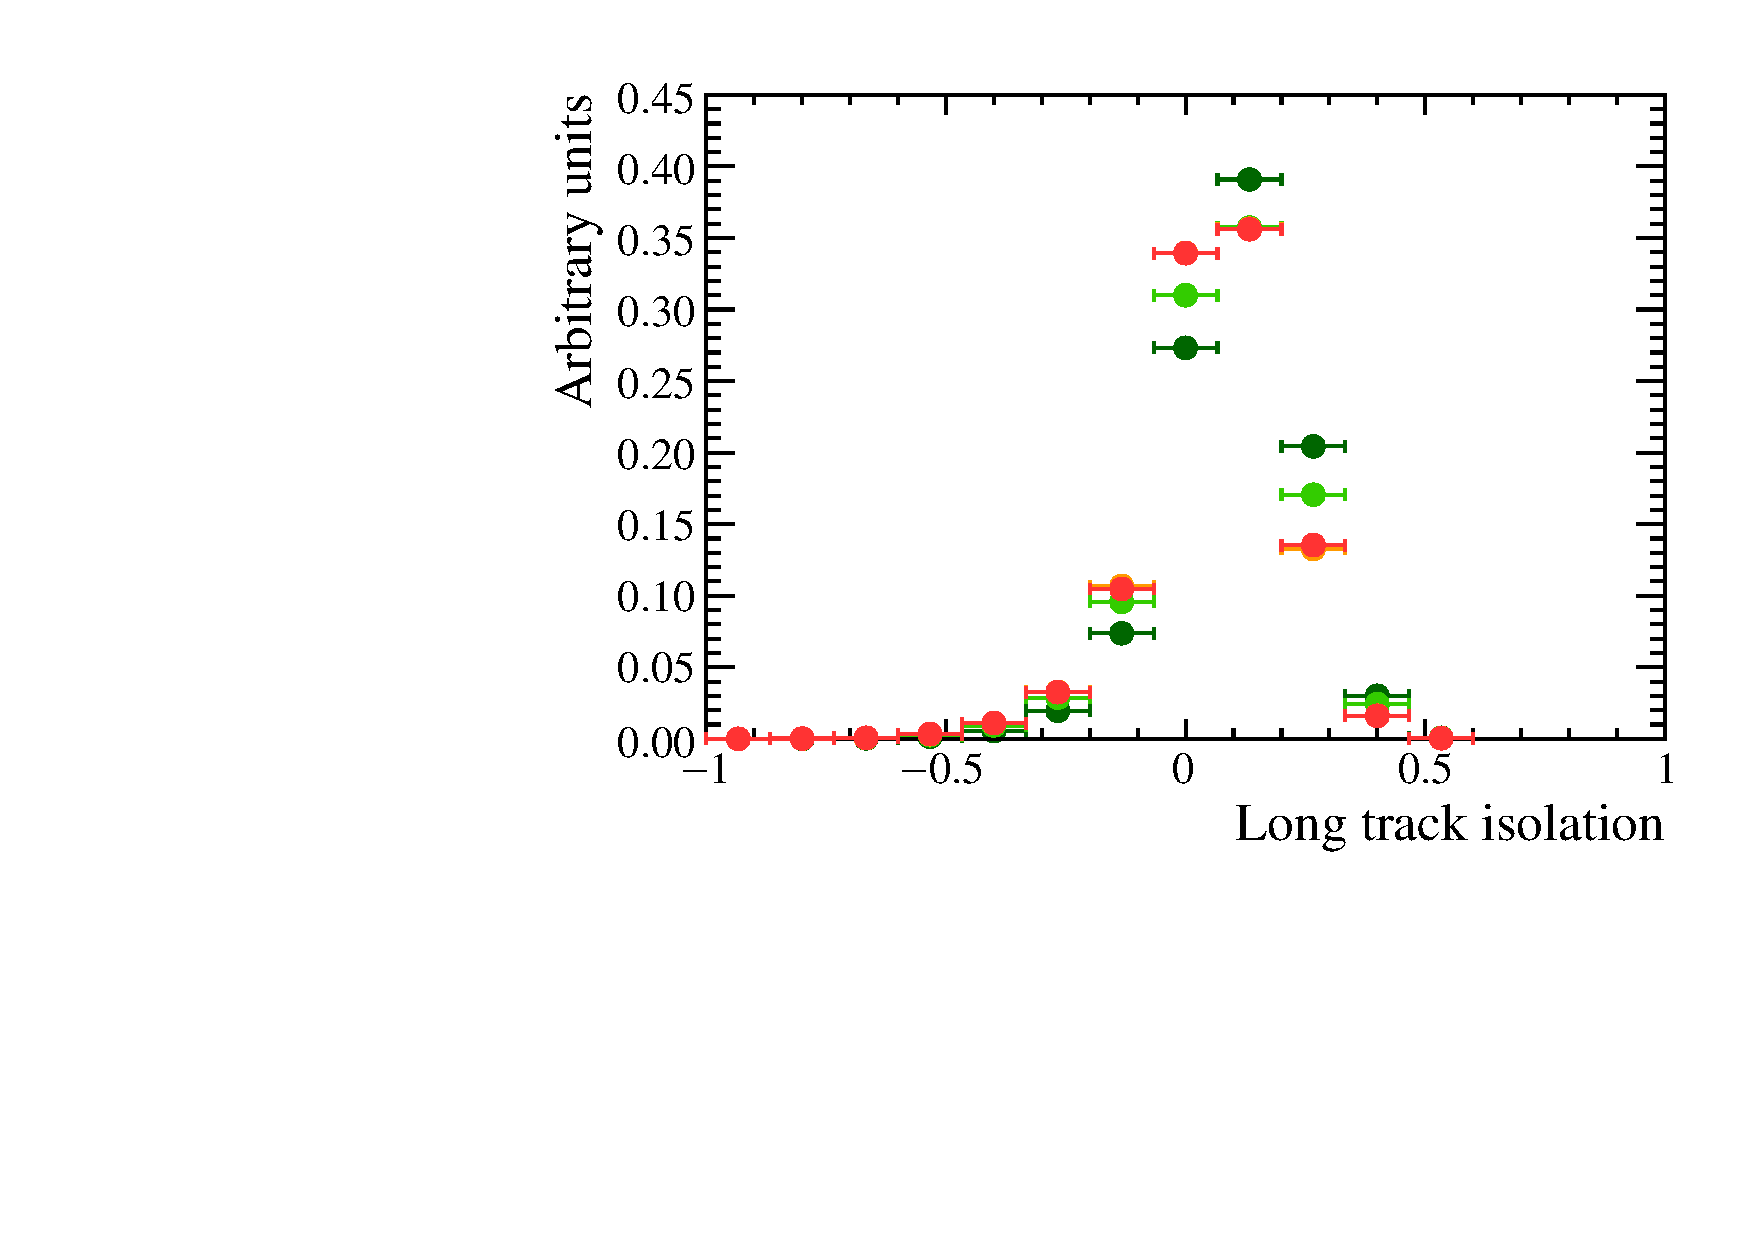
\includegraphics[width=\textwidth]{./Figs/Appendix1/signal_long_iso.pdf}
  %      \caption{ }
  %      \label{fig:BDTbkg}
    \end{subfigure}




 \begin{subfigure}[b]{0.48\textwidth}
        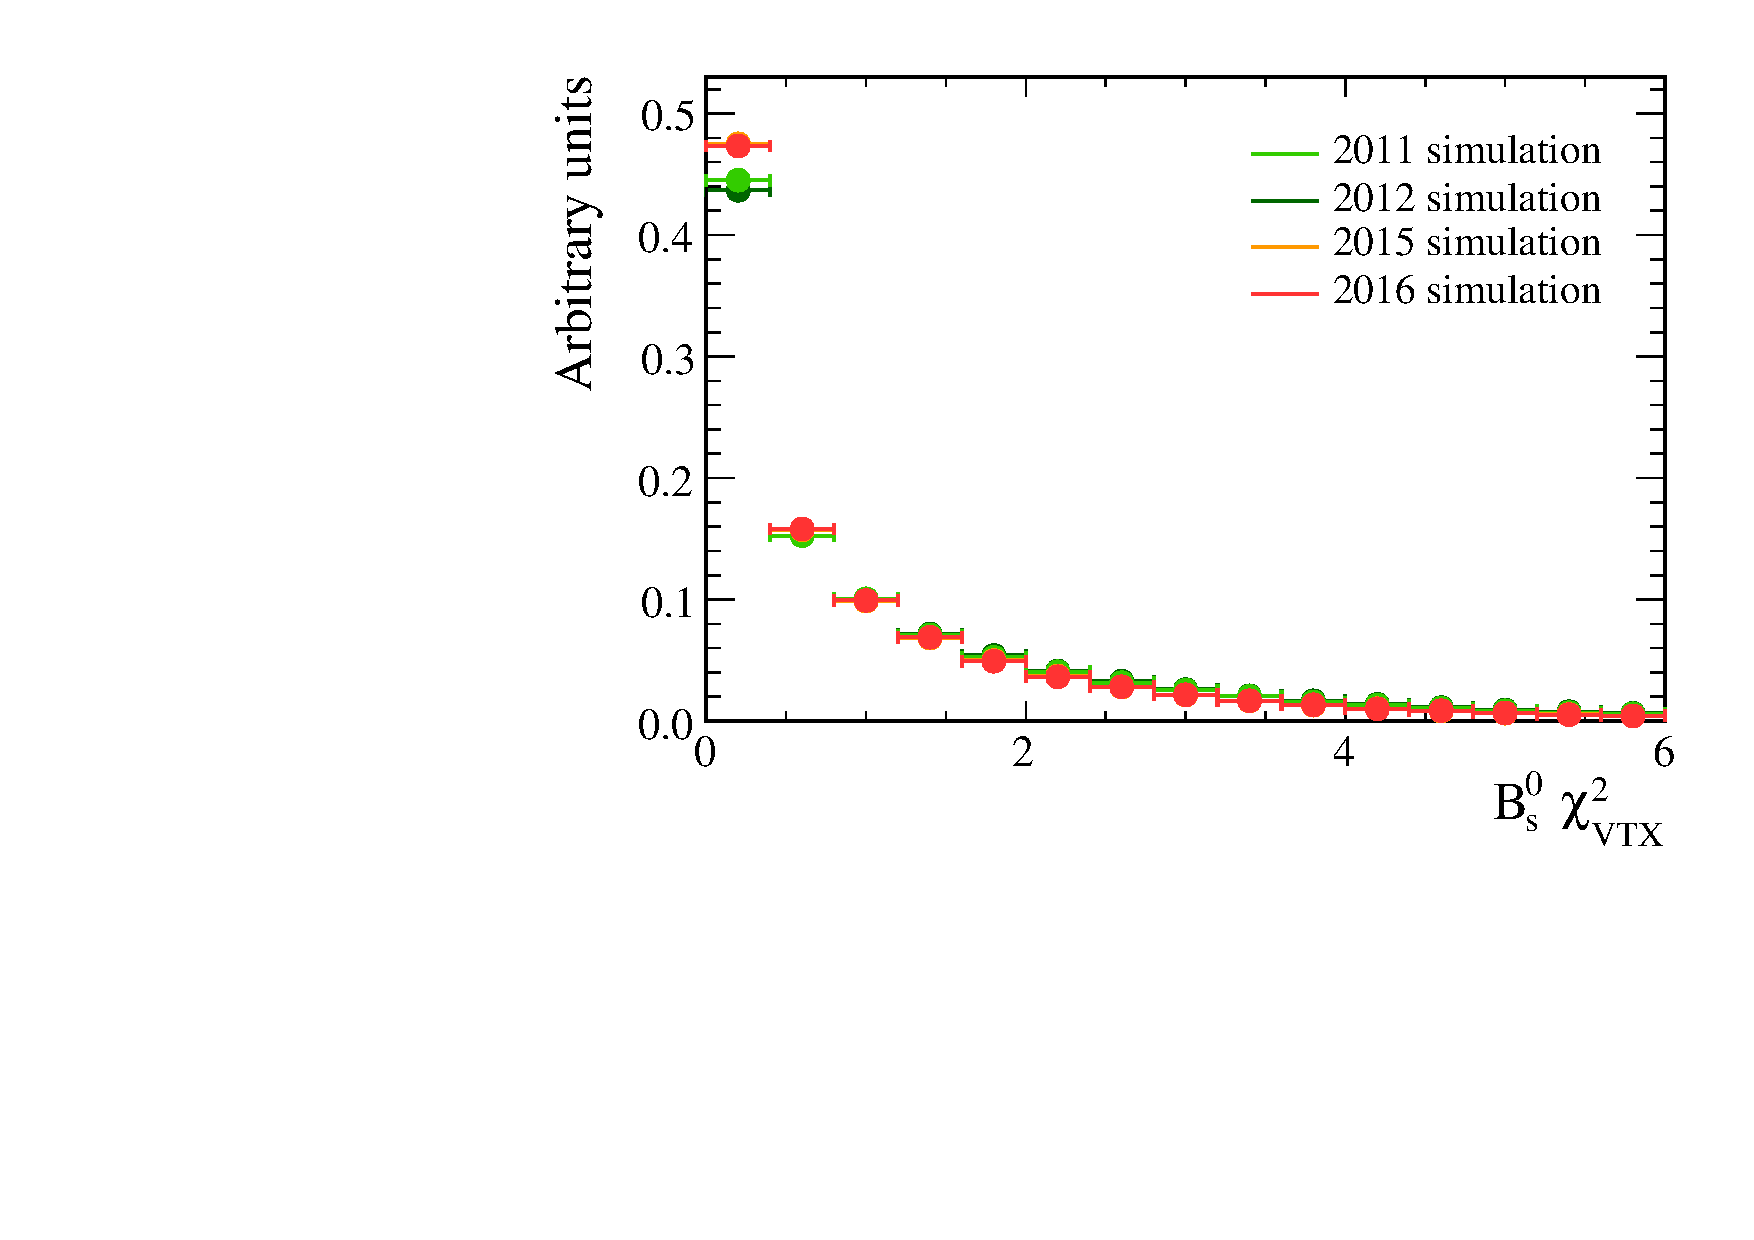
\includegraphics[width=\textwidth]{./Figs/Appendix1/signal_end_vertex.pdf}
   %     \caption{ }
   %     \label{fig:BDTsig}
    \end{subfigure}
    ~ %add desired spacing between images, e. g. ~, \quad, \qquad, \hfill etc. 
      %(or a blank line to force the subfigure onto a new line)
 



    \caption{Signal distributions for input variables for the global BDT for \bsmumu simulated decays in 2011, 2012, 2015 and 2016.}
    \label{fig:signalvars}
\end{figure}



\begin{figure}
    \centering
    \begin{subfigure}[b]{0.48\textwidth}
        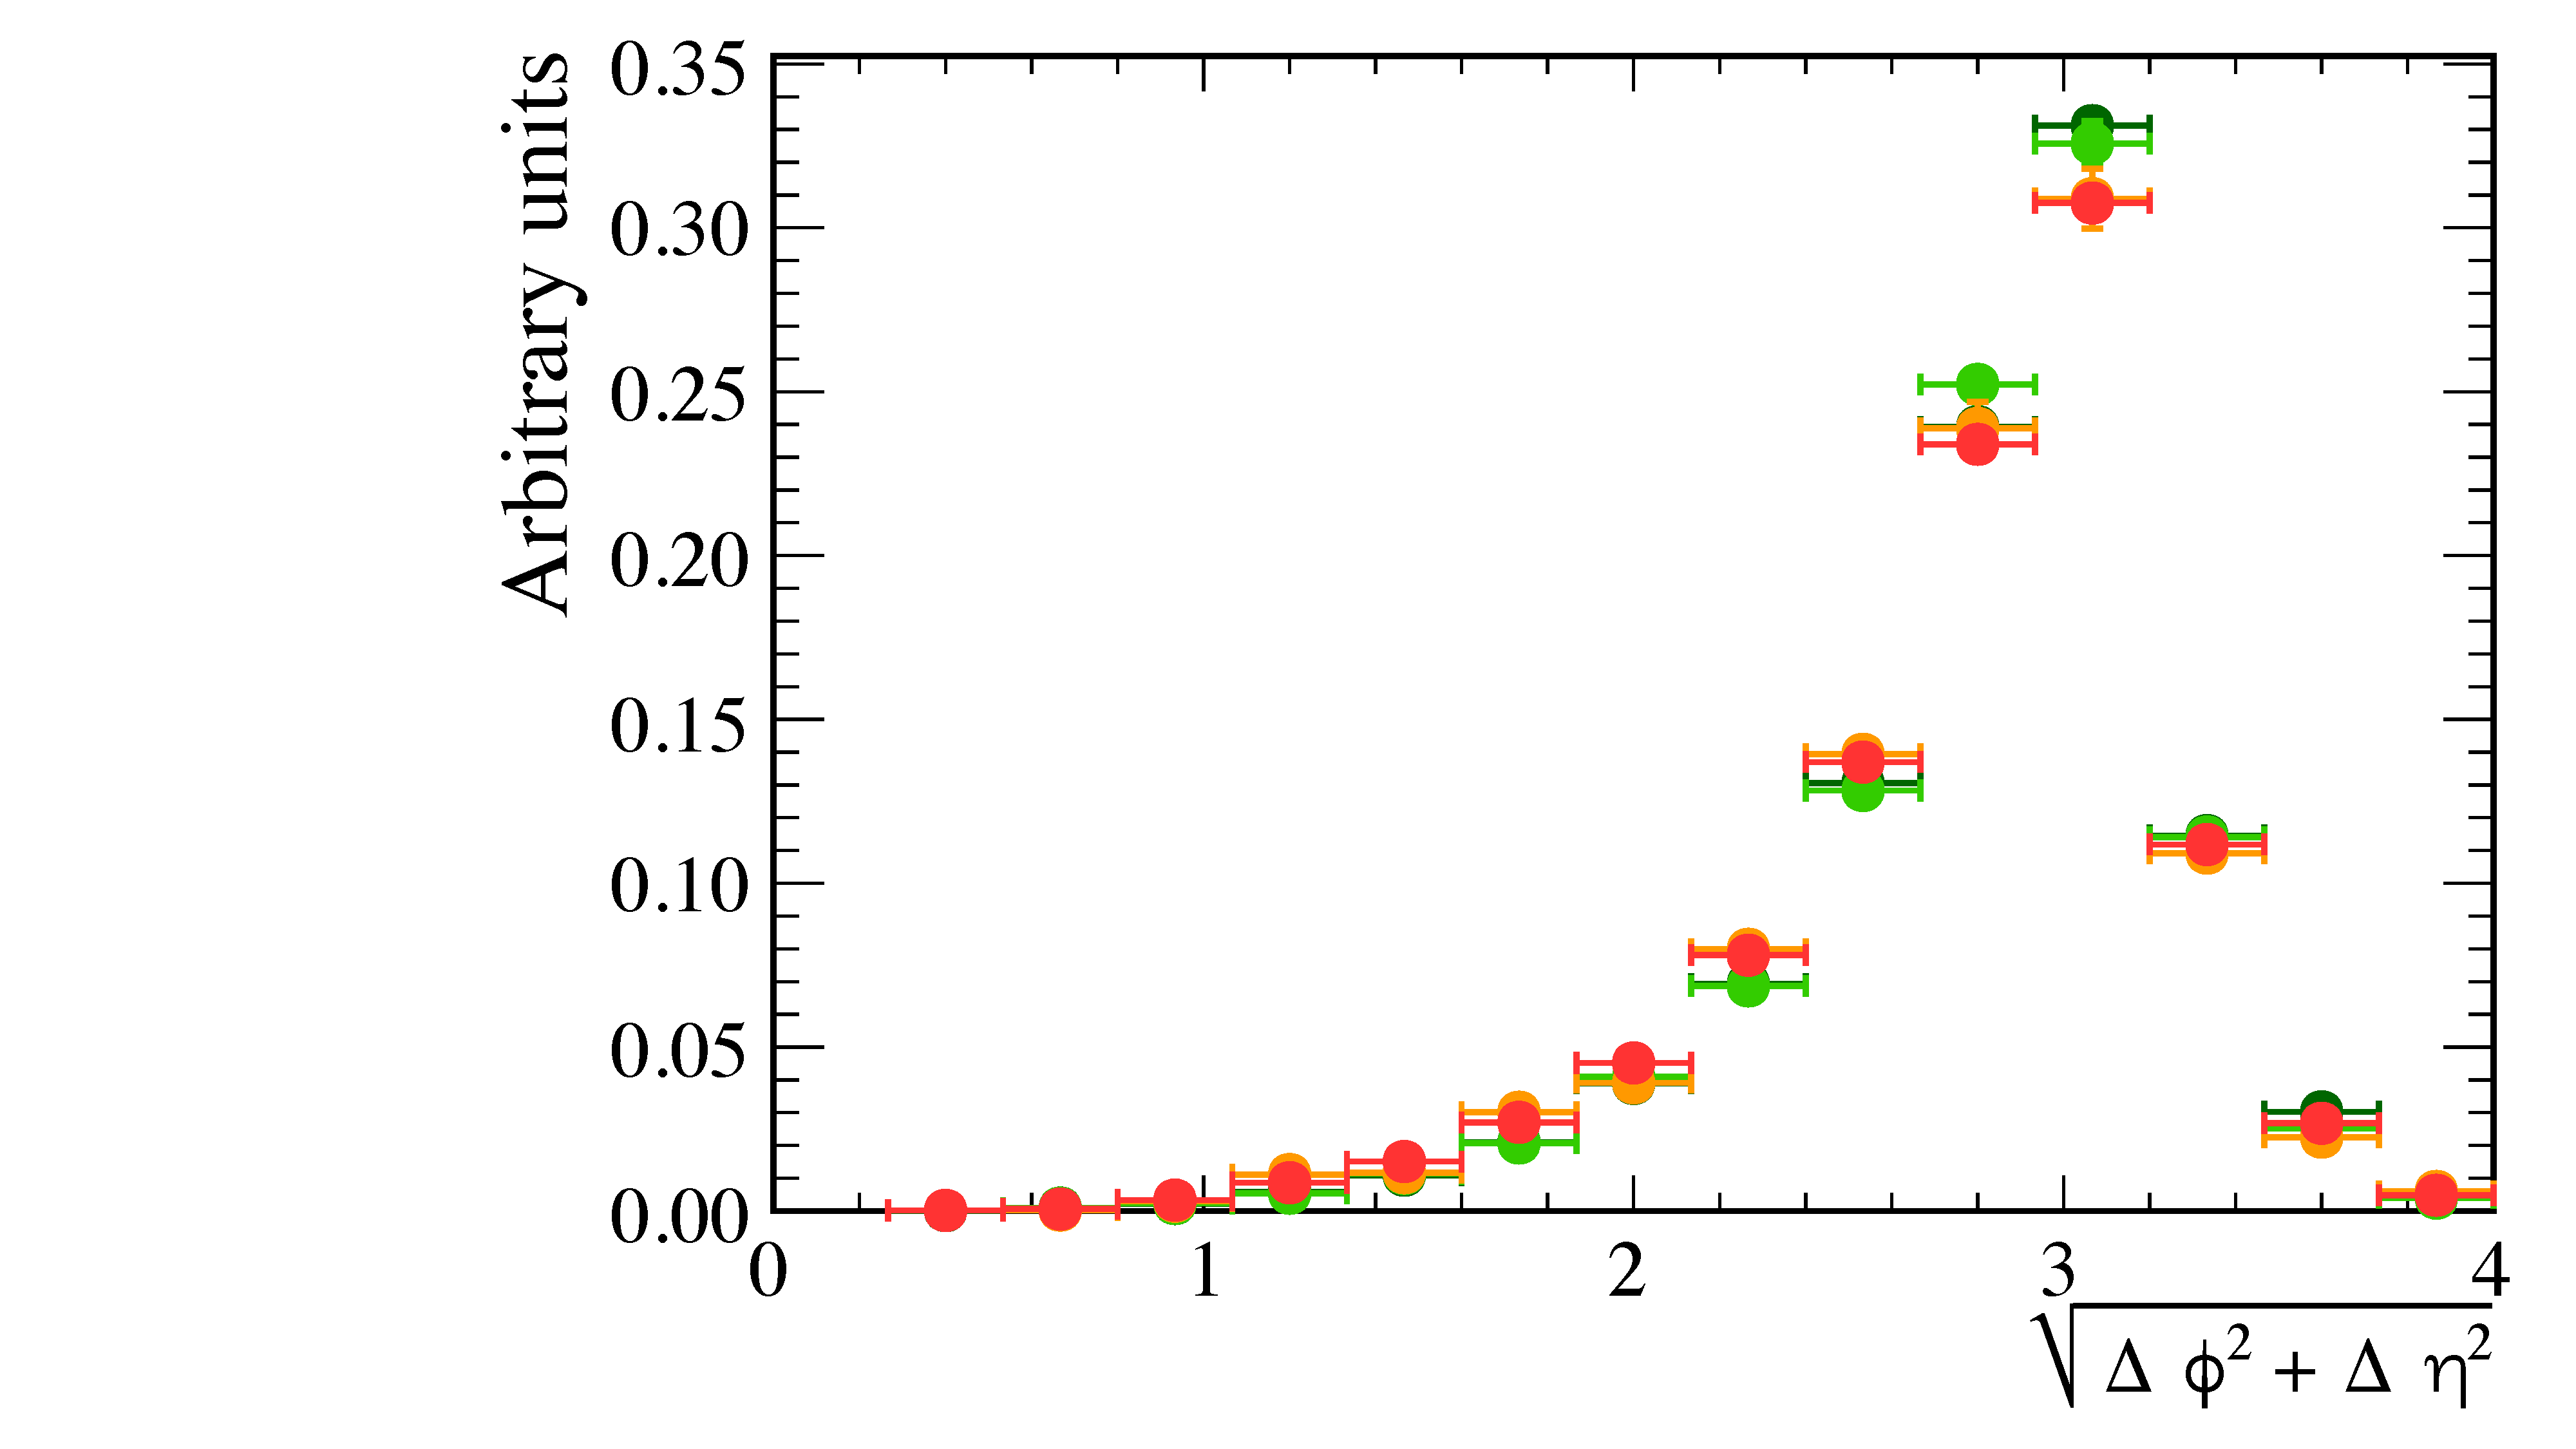
\includegraphics[trim={12cm 0 0 0},clip,width=\textwidth]{./Figs/Appendix1/bkgnd_DeltaR.pdf}
     %   \caption{ }
     %   \label{fig:BDTsig}
    \end{subfigure}
    ~ %add desired spacing between images, e. g. ~, \quad, \qquad, \hfill etc. 
      %(or a blank line to force the subfigure onto a new line)
    \begin{subfigure}[b]{0.48\textwidth}
       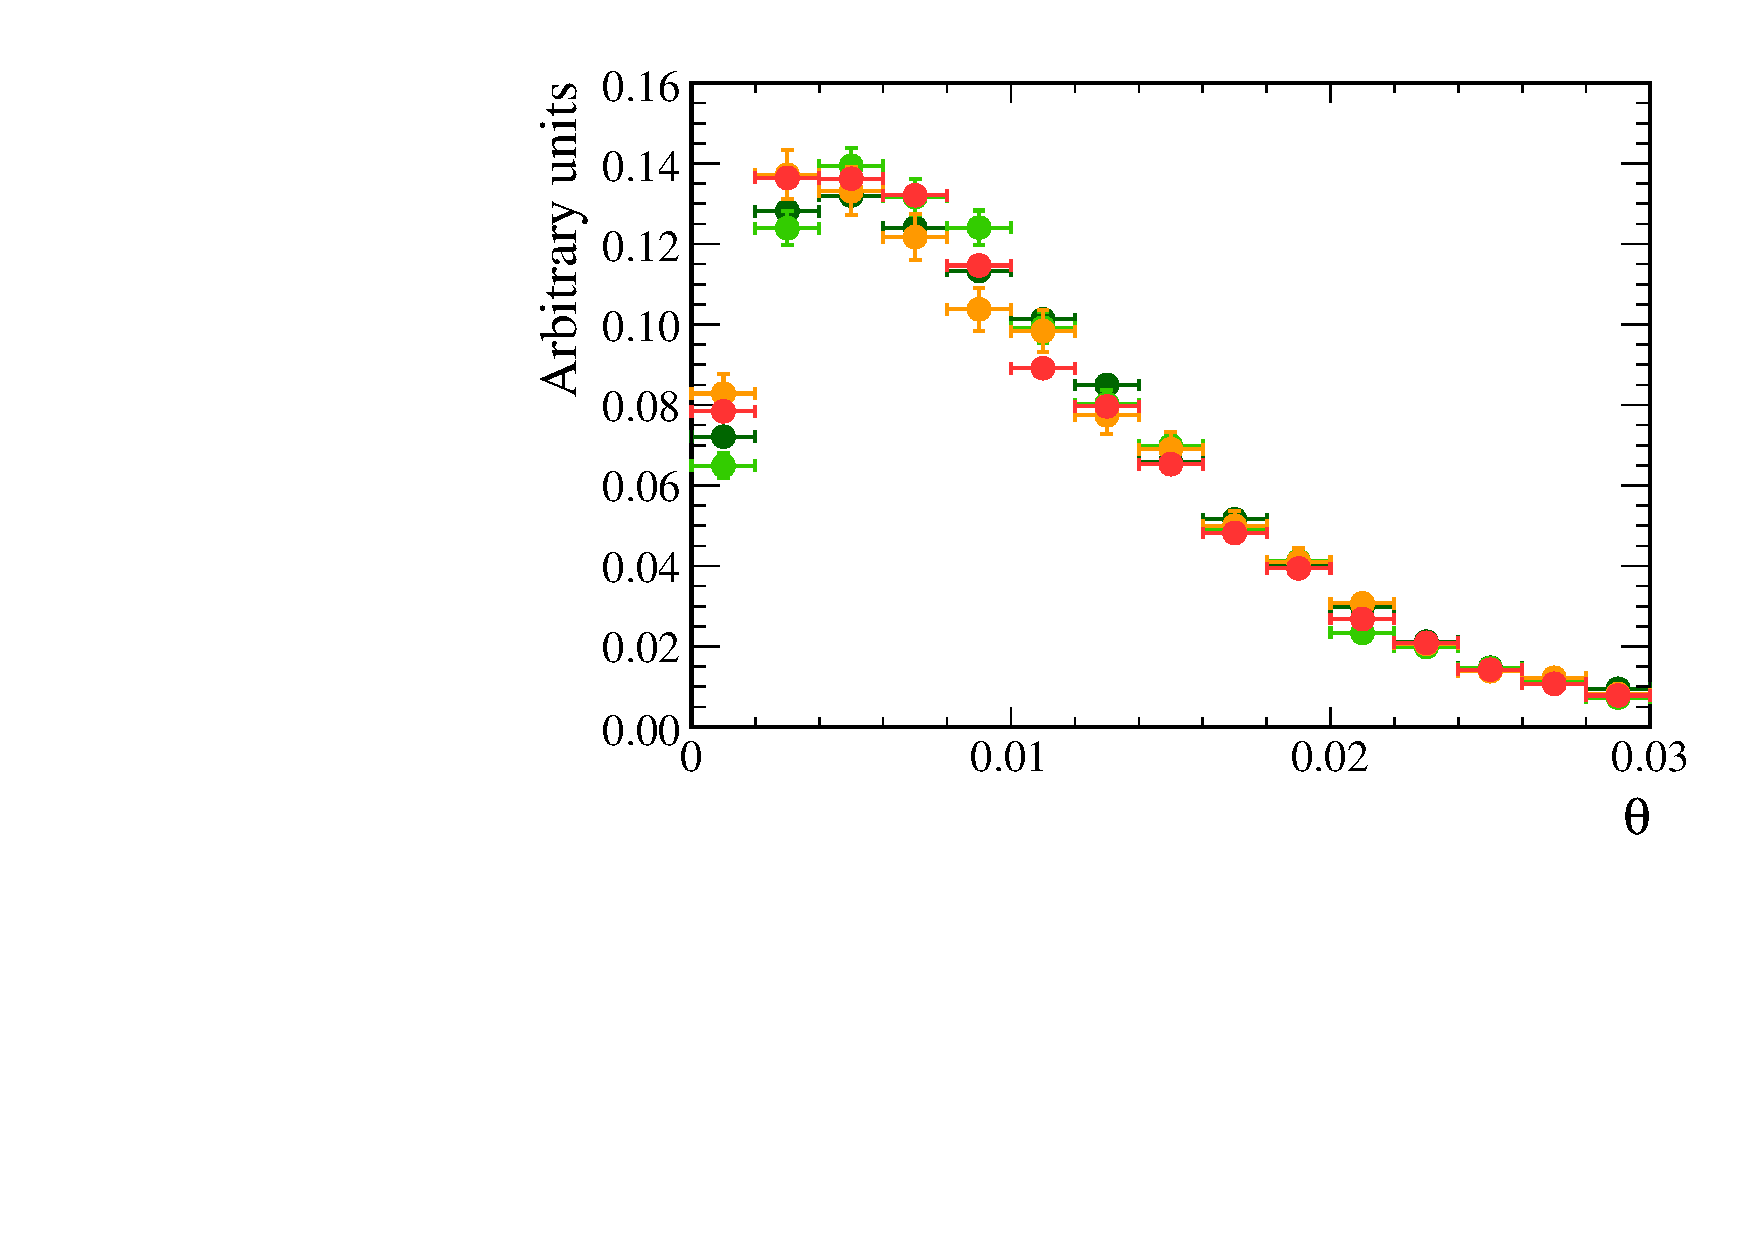
\includegraphics[width=\textwidth]{./Figs/Appendix1/bkgnd_DIRA.pdf}
    %    \caption{ }
    %    \label{fig:BDTbkg}
    \end{subfigure}



 \begin{subfigure}[b]{0.48\textwidth}
        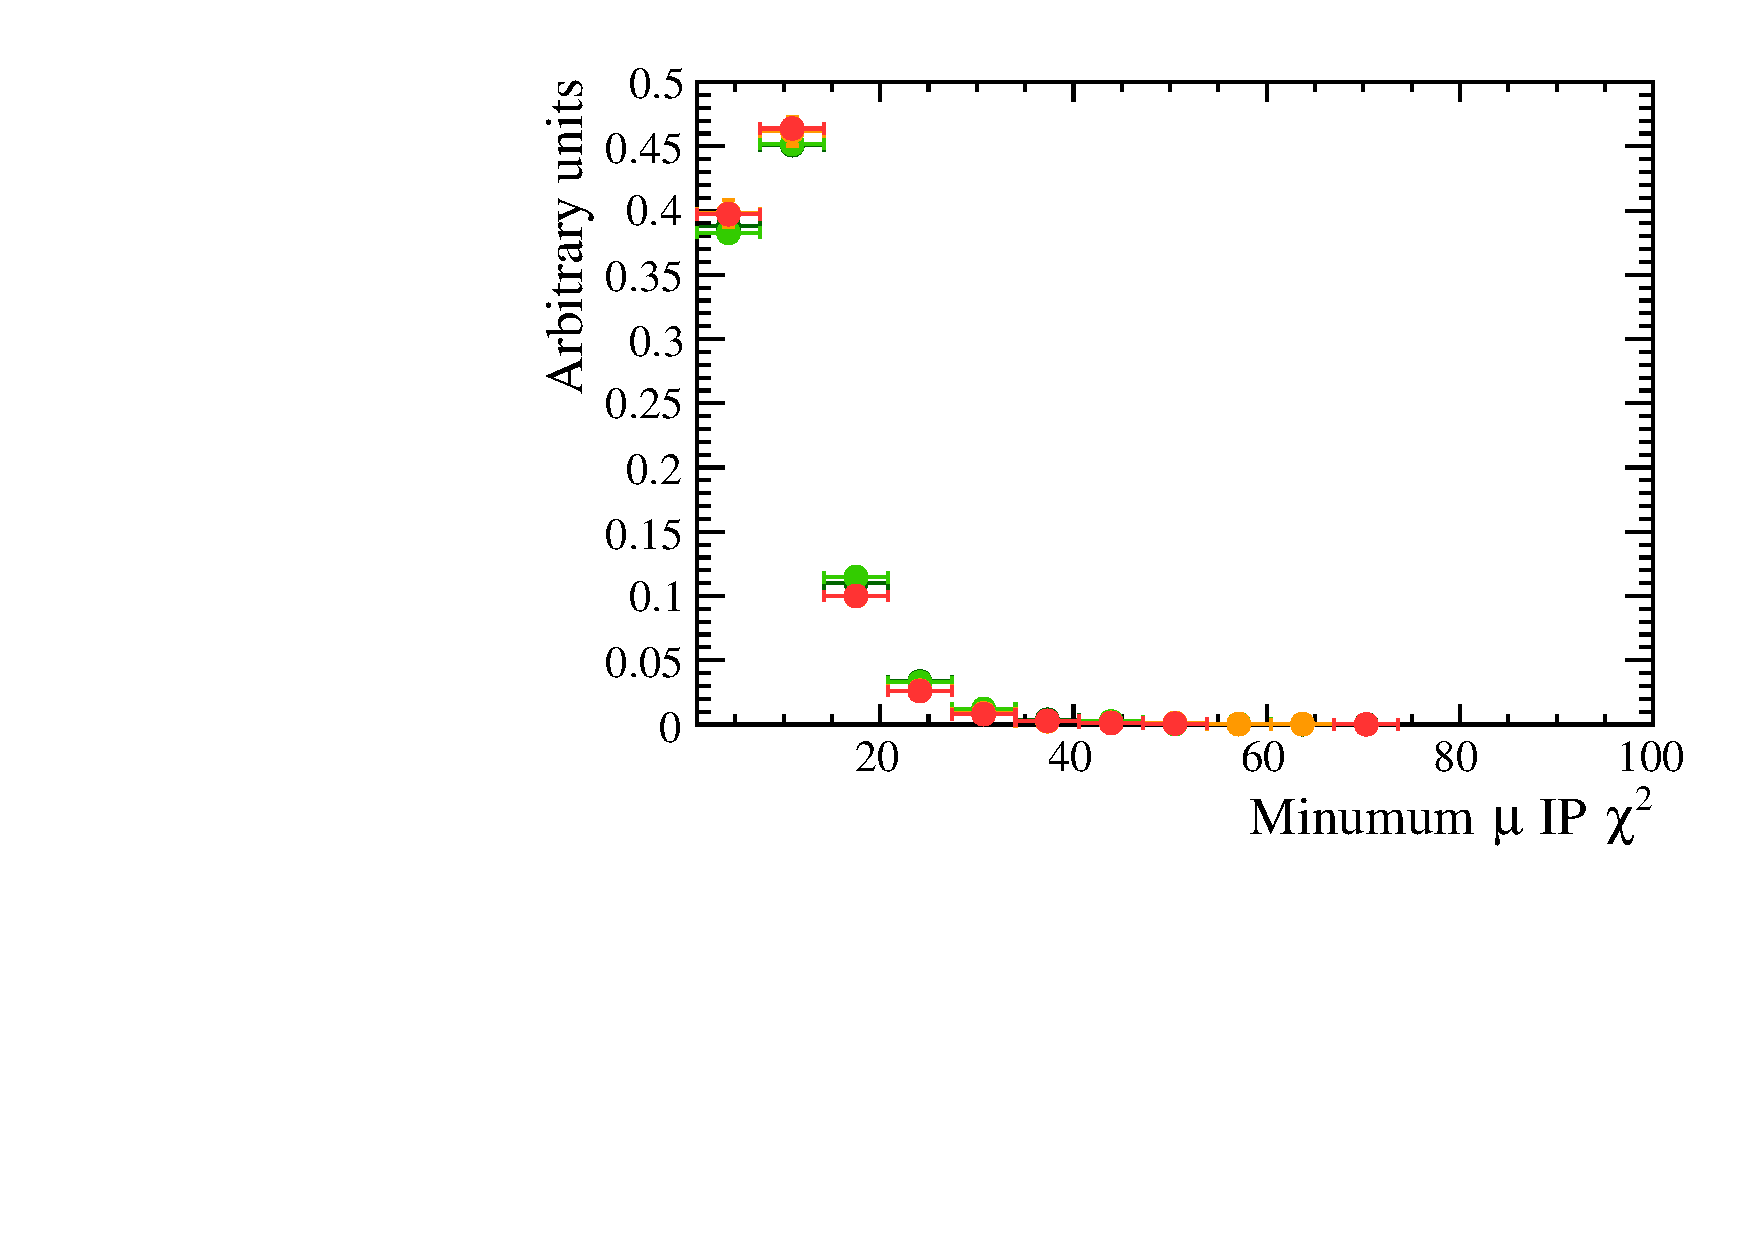
\includegraphics[width=\textwidth]{./Figs/Appendix1/bkgnd_muIPS.pdf}
      %  \caption{ }
      %  \label{fig:BDTsig}
    \end{subfigure}
    ~ %add desired spacing between images, e. g. ~, \quad, \qquad, \hfill etc. 
      %(or a blank line to force the subfigure onto a new line)
    \begin{subfigure}[b]{0.48\textwidth}
       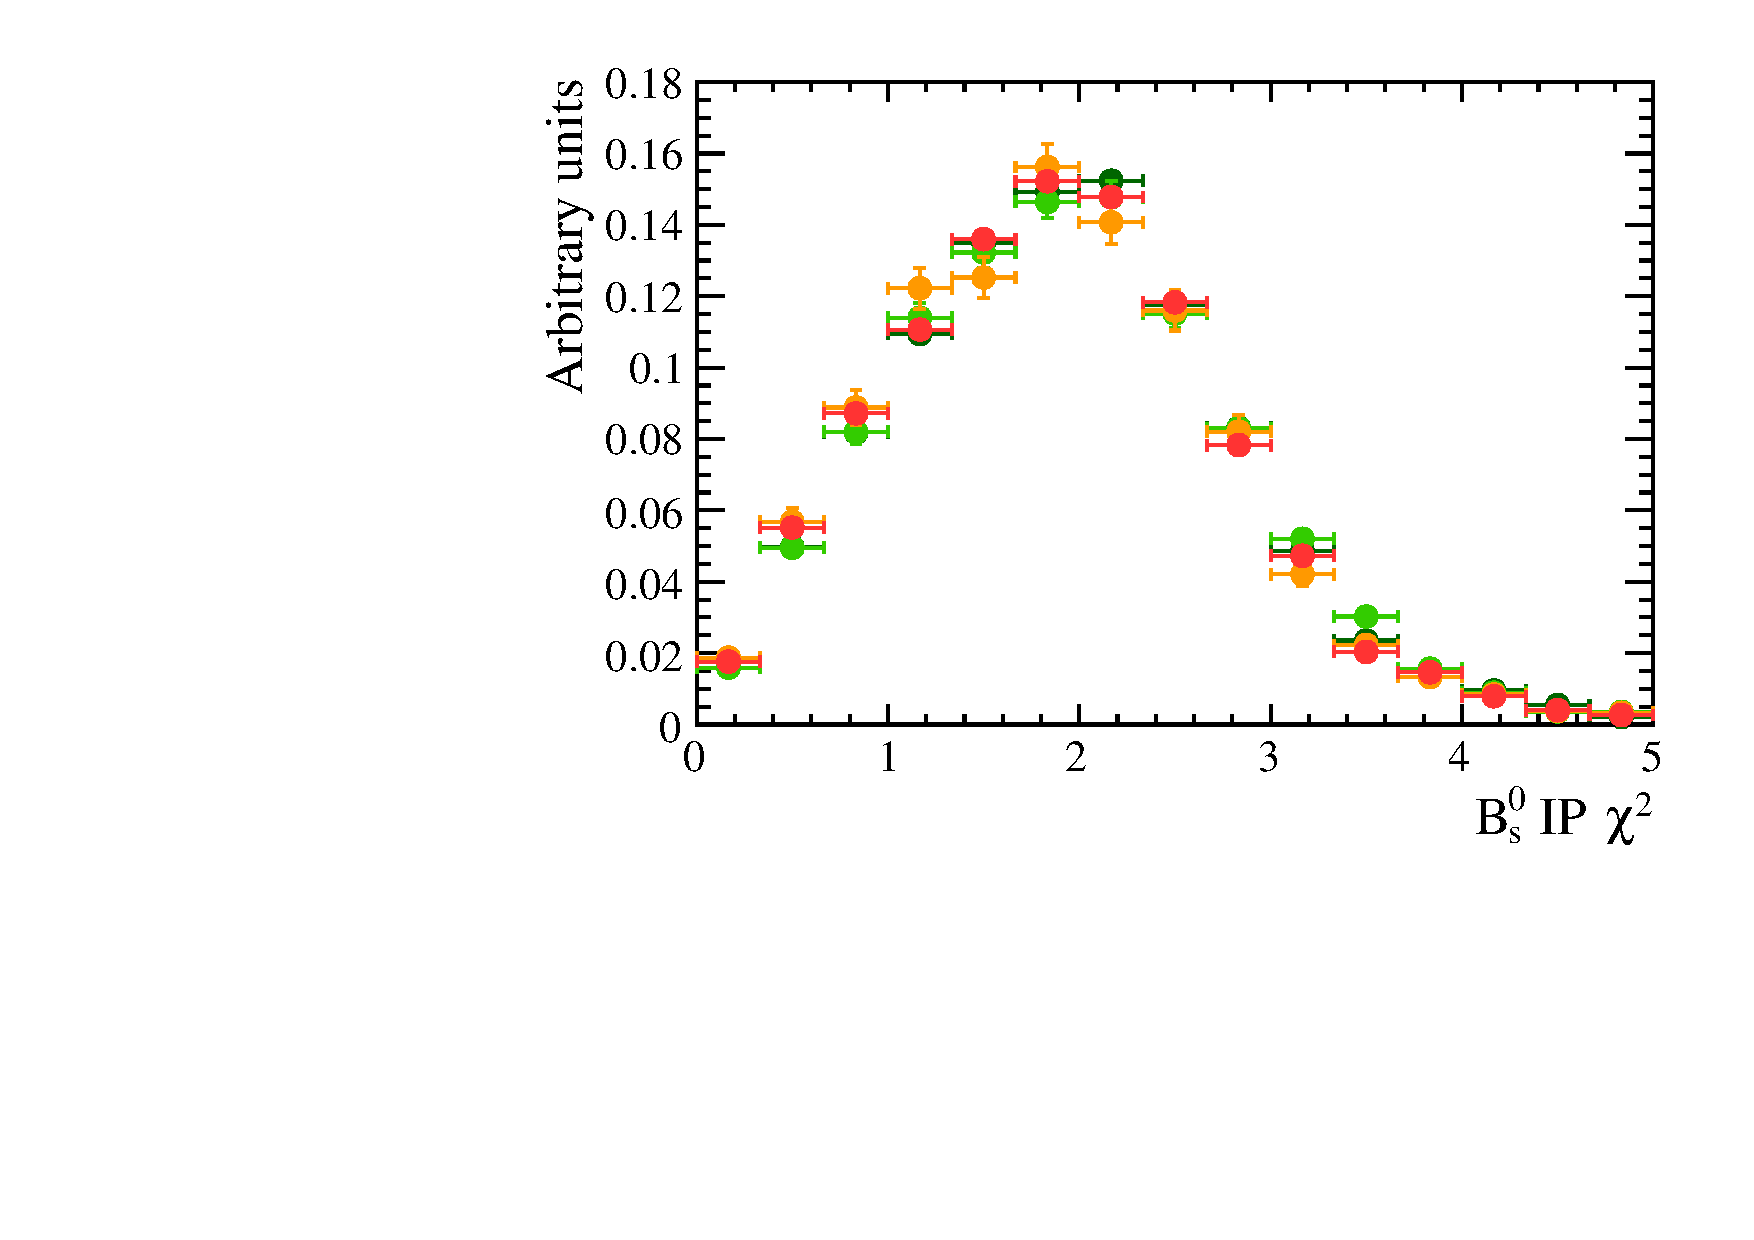
\includegraphics[width=\textwidth]{./Figs/Appendix1/bkgnd_IPS.pdf}
       % \caption{ }
       % \label{fig:BDTbkg}
    \end{subfigure}





 \begin{subfigure}[b]{0.48\textwidth}
        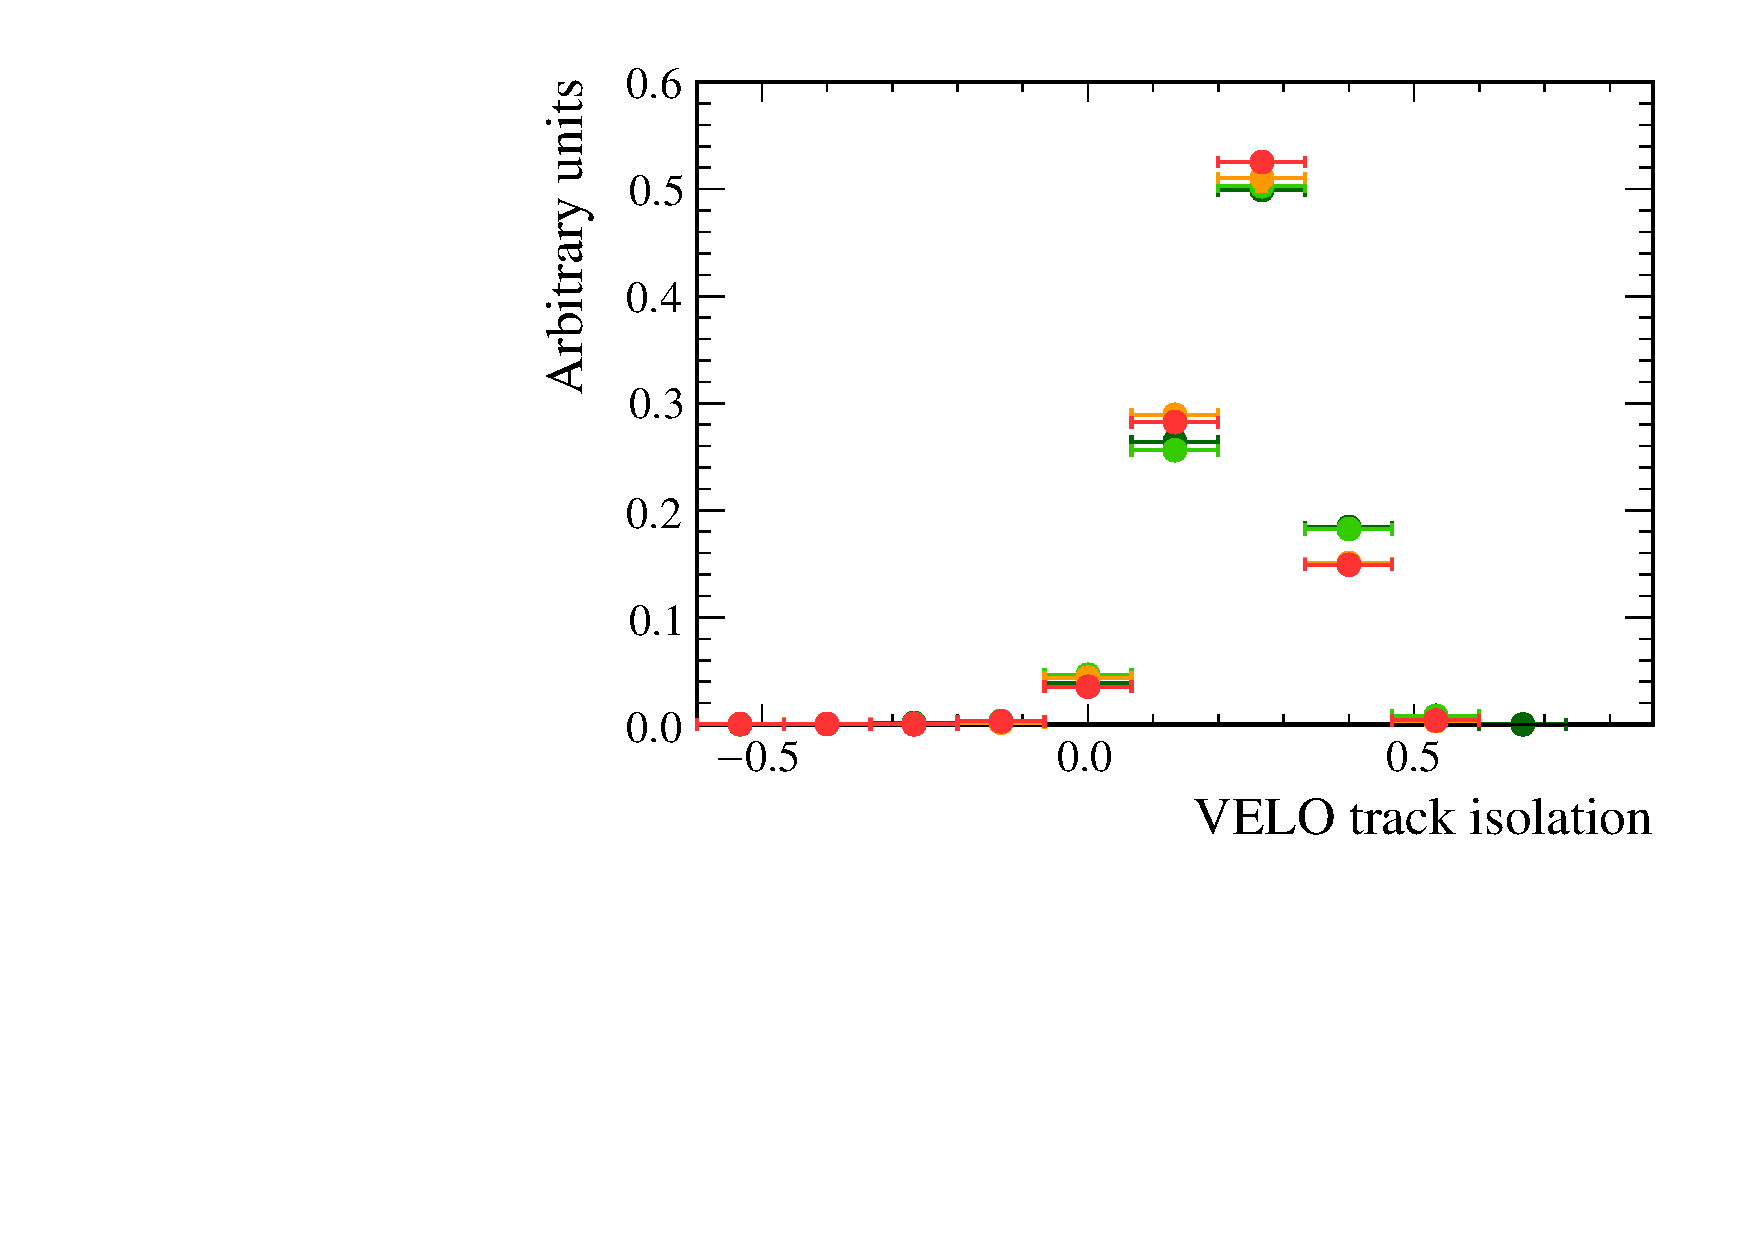
\includegraphics[width=\textwidth]{./Figs/Appendix1/bkgnd_iso_velo.pdf}
        %\caption{ }
        %\label{fig:BDTsig}
    \end{subfigure}
    ~ %add desired spacing between images, e. g. ~, \quad, \qquad, \hfill etc. 
      %(or a blank line to force the subfigure onto a new line)
    \begin{subfigure}[b]{0.48\textwidth}
       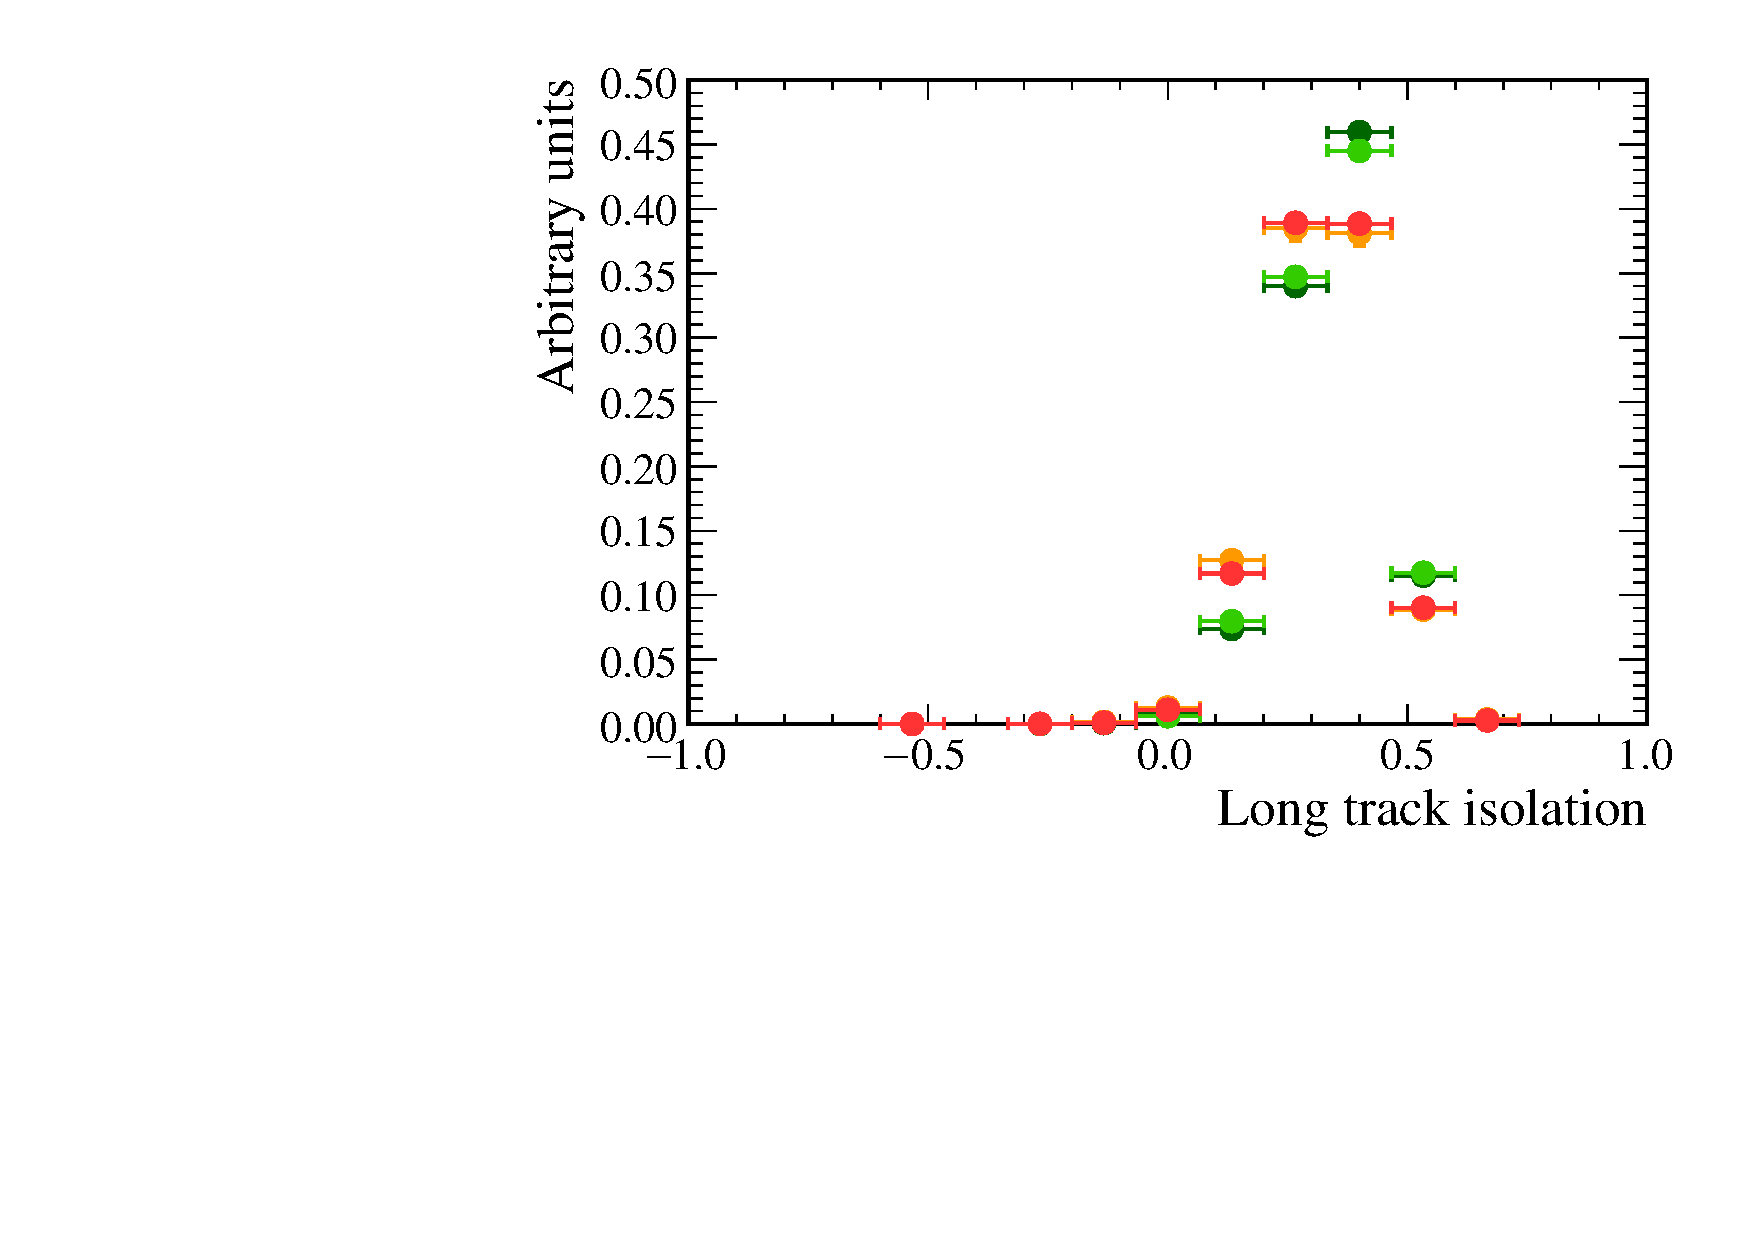
\includegraphics[width=\textwidth]{./Figs/Appendix1/bkgnd_long_iso.pdf}
        %\caption{ }
        %\label{fig:BDTbkg}
    \end{subfigure}




 \begin{subfigure}[b]{0.48\textwidth}
        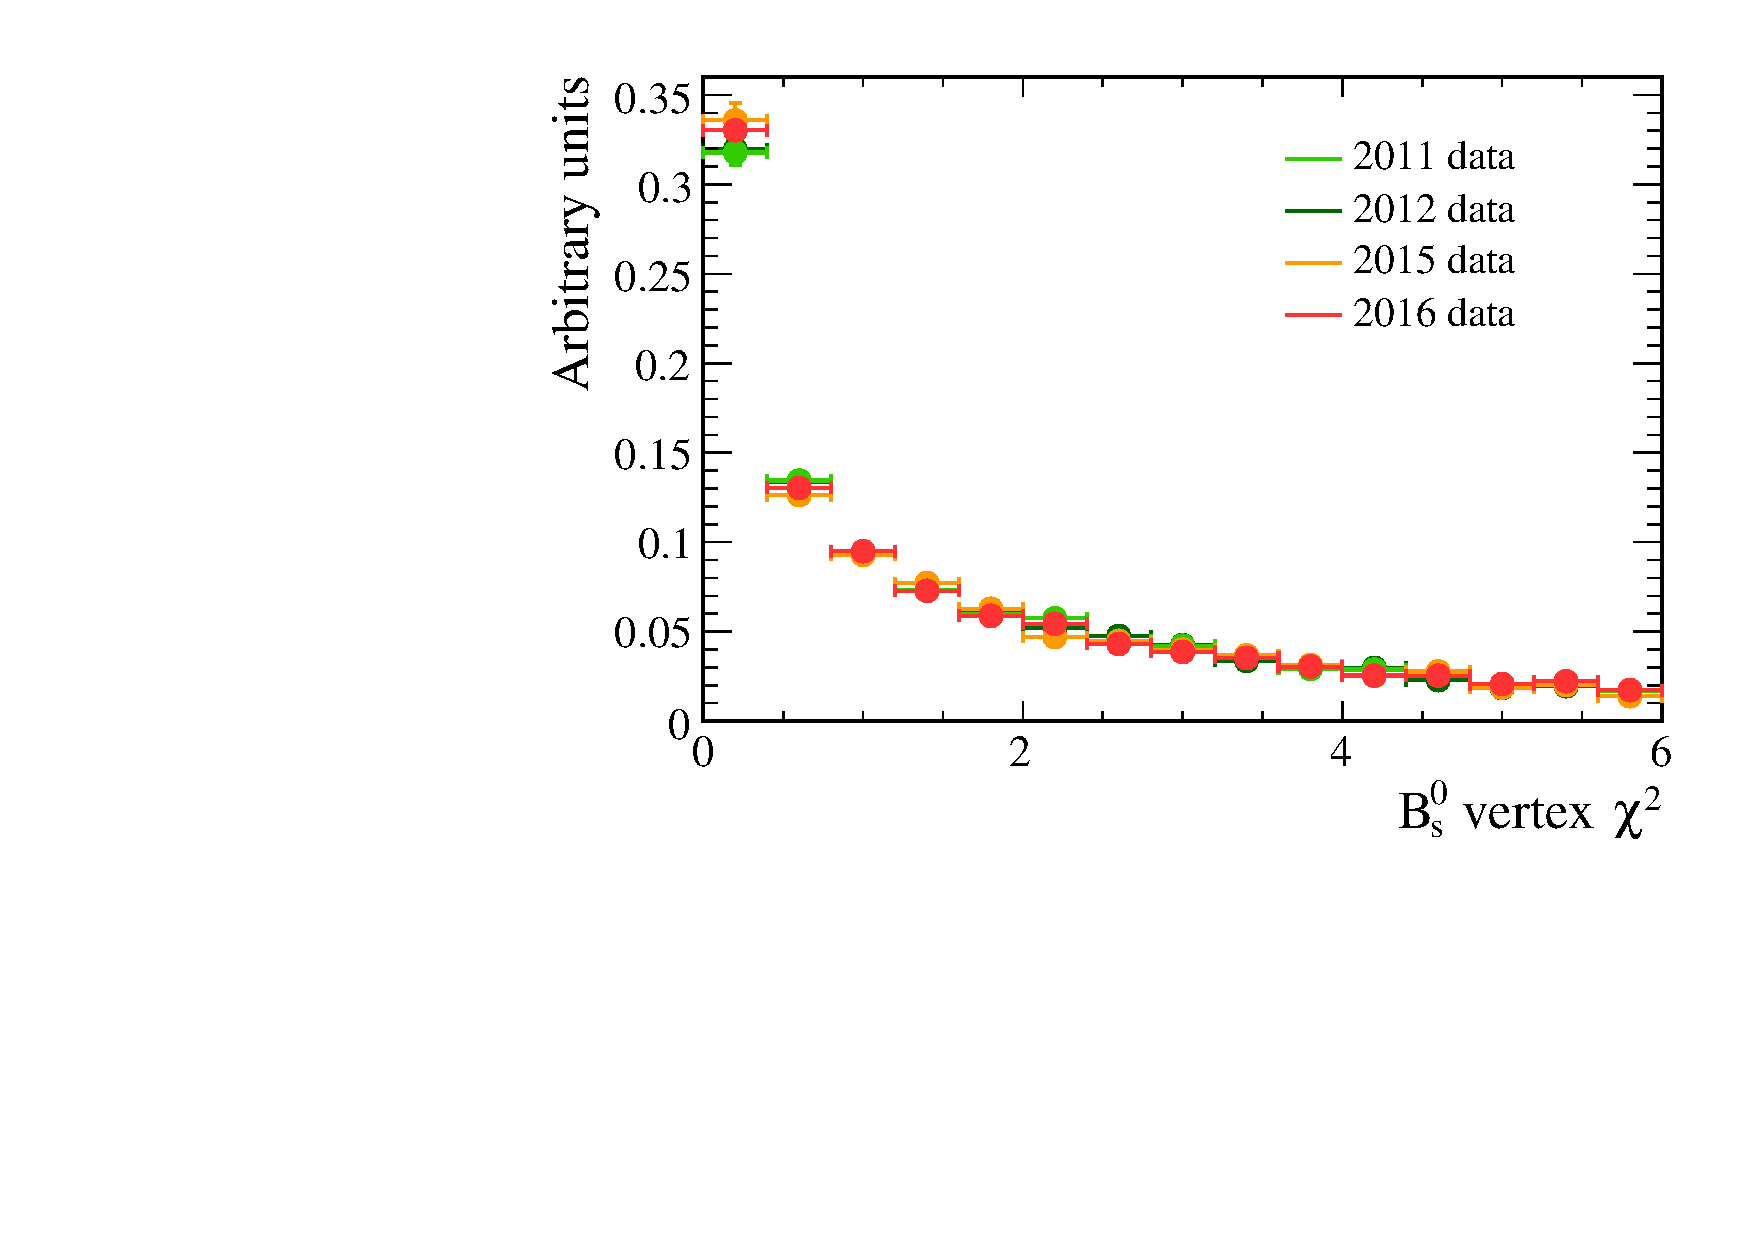
\includegraphics[width=\textwidth]{./Figs/Appendix1/bkgnd_vertex.pdf}
        %\caption{ }
        %\label{fig:BDTsig}
    \end{subfigure}
    ~ %add desired spacing between images, e. g. ~, \quad, \qquad, \hfill etc. 
      %(or a blank line to force the subfigure onto a new line)
 



    \caption{Background distributions for input variables from \bbbarmumux decays in 2011, 2012, 2015 and 2016 data with $m_{\mu \mu} > 5447$ \mevcc.}
    \label{fig:signalvars}
\end{figure}

%\chapter{Multivaraite Classifiers developed for the effective lifetime measurement}
\label{sec:appendix2}
%Details of the input variables used and the development of the classifiers.
%What need to go into here ...
%- put the reference for where the list of input variables were taken from
%- input variables used for the adaptive boost BDT with explaination of what they are, adding in references
%- input variables used for the uBoost BDT with explaination of what they are, adding in references
%- training parameters for both the uBoost and adaptive boost BDT
%- proof that the BDTs are not overtrained
%- discussion that different isolations are used but overall they don't change the conclusions.


%SO structure;
\section{Input variables}


%- the input variables were chosen in the following way
%- the starting set of variables were taken from .... but some others that were developed were added, these include isolation variables
%- The final set of input variables used in the adaptive boost BDT are, (put definitions next to each one and relevant references and also links to that chapters that explain what they are)
%- The final set of input variables used in the uBoost BDT are ... (same details as above)
%- Note that the BDT isolations are different from those used in the BF BDT, due to time constraints they set of varibles weren't re-optimised and also adding them in made the gloabl BDT still performs best

%CDF isolation~\cite{Abulencia:2005pw}, ZViso (Alessio's thesis)~\cite{Mordà:2120795} he also has an explaination of the CDF isolation and the others, original list of input variables~\cite{AdroverPacheco:1481060}
%Prehaps reference the internal note for the isoBDTs?


The input variables used in the adaptive boosting and uBoost BDTs were chosen separately, starting from a large set of variables including kinematic, geometric and isolation variables. Initially the BDTs were trained using all input variables within the set and variables that had no impact on the BDT performance were removed until removing any of the remaining variables had a negative impact on the BDT performance. Each BDT performance was evaluted from the integreated Receiver Operating Charateritic curve, which is the signal efficiency versus (1 - background rejection). The inital set of input variables tested were based on the variables used in~\cite{Abulencia:2005pw}} and new isolation variables that were developed for the study of \bmumu decays. 


The adaptive boosting BDT uses 11 input variables and the uBoost BDT uses 21 variables which includes the adaptive boosting BDT varaibles.
The input variables used in both algorithms are related to the \bs, the muons and isolation variables. Some of the input variables used are also in used in the cut based selection, these variables are; 
\begin{itemize}
\item impact parameter and impact parameter \chisqd of the \bs
\item vertex fit \chisqd/$ndof$ of the \bs 
\item the flight distance \chisqd of the \bs
\item the transverse momentum of the \bs and the minimum transverse mometum of the two muons
\item the minimum impact parameter significance of the two muons
%\item the polerisation angle which is the cosine of the angle between a vector perpendicular ot the plane containing the \bs momentum and the beam axis and the muon momentum in the \bs rest frame
\end{itemize}
The definitaion of these variables are given in Section~\ref{strippingold}. The additional variables not used in the cut based selection are;
%Many of these variables used in the stripping selection and the definitions are given in Section~\ref{strippingold}. 
\begin{itemize}
\item  the polerisation angle which is the cosine of the angle between a vector perpendicular otthe plane containing the \bs momentum and the beam axis and the muon momentum in the \bs rest frame 
\item $(\Delta \phi)^{2}$ where $\Delta \phi$ is the difference in azimuthal angles of the muons\item a BDT based isolation variable designed in the same way was those described in Section~\ref{sec:globalBDT}, using information from long (?) tracks. This isolation version was produced during the development of the final isolations used in the global BDT, the details of this variable can be found in~\cite{Archilli:1970886}. \footnote{Replacing this isolation variable with the Long track and VELO track isolations does no significantly improve the overall BDT performance.}
\item isolation variable ({\it ZViso}) which uses a topological vertex algorithm and is defined in~\cite{Morda:2120795}
\end{itemize}

The additional input variables used in the uBoost BDT are;
\begin{itemize}
\item $(\Delta \eta)^{2}$, where $\Delta \eta$ is the difference in the pseudorapidity of the muons
\item an isolation variable of the \bs candidate based on the definition use by the CDF collaboration in the search for \bmumu decays~\cite{Abulencia:2005pw}. The isolation is computed from the transverse momentum, $p_T$ of the \bs and all tracks in an event within a cone around the \bs, the isolation is defined as
\begin{equation}
I_{CDF} = \frac{p_{T}(B_{s}{^0})}{p_{T}(B_{s}{^0}) + \displaystyle\sum_{track \in cone}p_{T}(track) }
\end{equation}
where the cone is 
\begin{equation}
\sqrt{\delta \eta^{2} + \delta \phi^{2}} > 1.0
\end{equation}
$\delta \eta$ and $\delta \phi$ are the differences in pseudorapidity and azimuthal angle of a track in the events and the \bs candidate (This is very simlar in layout to Alessio's)
\item a cut based muon isolation, this isolation varibale was the precursor of the BDT based isolation variables and is based on placing cuts on variables relating long tracks in the event to the muons in \bsmumu candidates. The definition of this variable can be found in~\ref{Mordà:2120795}} %isolation_Giampi
\item %B_otherB_ang
\item %B_otherB_boo_ang
\item four jet based variabes %B_JETBJETWIDTH, B_JETBPT, B_JETBPTRATIO, B_JETMU1DRMU2
\item the direction cosine, DIRA, as defined in~\red{strippingold}
\end{itemize}

\section{Training parameters}
%- The training parmeters used in the final BDTs trained on data are ....
The training parameters discussed in Section~\ref{sec:GeneralBDT} put constraints on how a BDT sperates signal and background decays. 
The training parameters used in the adaptive boost BDT were optimised by iterating over different training parameter values and chosing the BDT which gave the best signal significance for identifyting \bhh decays in Run~1 data. The computation of the signal significance is described in Section~\ref{sec:dev_BDTs}. %The training parameters were optimised one-by-one in the order NCuts, NTrees, MinNodeSize, MaxDepth the $\beta$, the default TMVA values were taken as the starting point.
The final set of training parameters are given in Table~\ref{tab:ELtrainingparamss}. %{\it I can find the book with this in and add a few more details?}
The training parameters used in the uBoost BDT have not been optimised and are given in Table~\ref{tab:ELtrainingparamss}. The parameter values suggested in~\cite{Stevens:2013dya} have been used where is was shown that different training parameters had a small impact of the overall BDT performance. %are given in Table~\ref{}, the parameters are taken from~\ref{} and have no alternative parameters were investigated because little improvment can be gained for this algorithm by altering the training parameters.
\begin{table}[htbp]
\begin{center}
\begin{tabular}{ll|ll}
\hline
\multicolumn{2}{c}{Adaptive Boost BDT} & \multicolumn{2}{c}{uBoost BDT} \\ \hline
Parameter & Value & Parameter & Value\\ \hline
nTrees & 1000 &  nTrees & 100\\
%nEventsMin & 400 \\                                                                                                                                                                
MinNodeSize & 5$\%$ & nEventsMin & 100 \\
MaxDepth & 3 & MaxDepth & 4 \\
%NNodesMax = 100000 \\                                                                                                                                                              
$\beta$ & 0.1 & $\beta$ & 1.0 \\
nCuts & 30 & nCuts & 200 \\
\hline
\end{tabular}
\vspace{0.7cm}
\caption{Training parameters used to specify the training of the adaptive boost and uBoost BDT.}
\label{tab:ELtrainingparamss}
\end{center}
\vspace{-1.0cm}
\end{table}


\section{Overtaining test}
%- Overtaining of the BDTs
As discussed in Section~\ref{sec:GeneralBDT}, it is important that BDTs are not overtained. %To test this the signal and background samples are split into two and half of the signal and background samples are used to train a BDT, the BDT is then applied to the other half of the signal and background samples. 
The BDT output value is evaluted for each decay in the sample and the output values are compared for both s
To test this assumption the signal and background samples are both split in two to create a training set and a testing set.
A BDT is trained using the training set, and the BDT is then applied to both the traning and testing sets. The distribution of BDT output values for signal and background decays inthe training and testing sets are compared. If the BDT is overtrained the response of the BDT will be quite different for the training and testing sets for signal and background decays, however is the BDT is not overtrained the distributions will be similar for the training and testing sets. 

Figure~\ref{fig:ELBDTovertrain} shows the results of this test which is performed using the TMVA package~\cite{Hocker:2007ht}, neither the uBoost BDT of the adaptive boosting BDT developed for the effective lifetime measurement are overtrained. %The same test was performed for the global BDT developed of the \BFm and the results are shown in Figure~\ref{}, the global BDT is not overtrained.  

%The output values of the BDT for the set of decays used in training is compared to the output values of the set of decays not used in training. 
\begin{figure}[htbp]
   \centering
        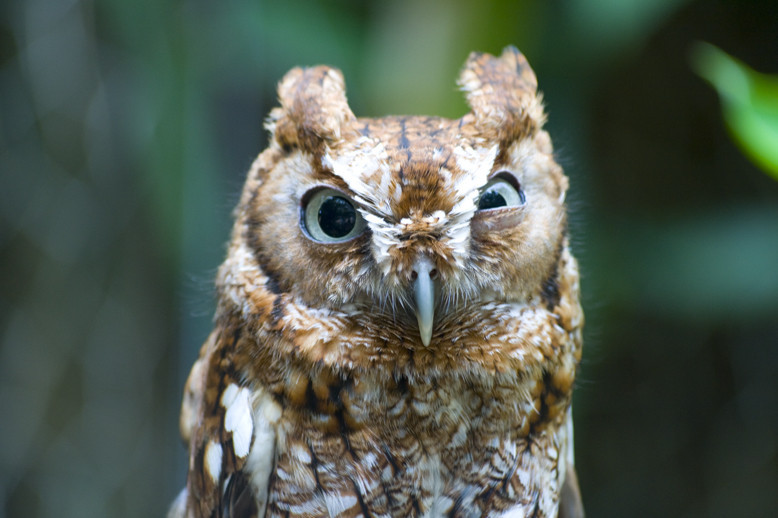
\includegraphics[width=0.49\textwidth]{./Figs/placeholder.jpeg}
        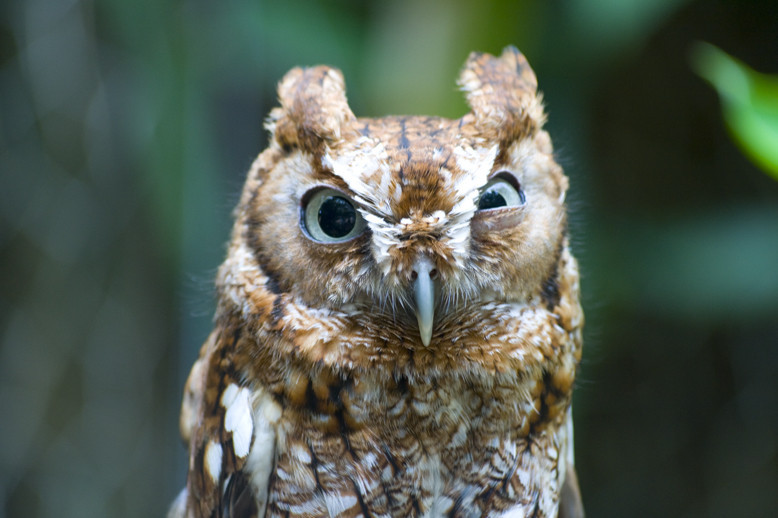
\includegraphics[width=0.49\textwidth]{./Figs/placeholder.jpeg}

    \caption{BDT response for training and testing samples of signal and background decays for the adaptive boost BDT (left) and the uBoost BDT (right). }
    \label{fig:ELBDTovertrain}
\end{figure}



%\begin{figure}[htbp]
%   \centering
%        \includegraphics[width=0.6\textwidth]{./Figs/Appendix2/}
%    \caption{BDT response for training and testing samples of signal and background decays for the global BDT~cite{}. }
%    \label{fig:BFBDTovertrain}
%\end{figure}





\end{appendices}

% *************************************** Index ********************************
\printthesisindex % If index is present

\end{document}
